%%%*******************************************************************************
%  Classe Latex THEOPRAX, Version 0.0.0 31/10/2017
%
%  Define as normas e estilo das dissertações, teses ou tcc do SENAI CIMATEC
%
%%%-------------------------------------------------------------------------------

%%%-------------------------------------------------------------------------------
% Changes log
%%%-------------------------------------------------------------------------------
% Version 0.0.0 - 00/00/2000
% - 
%%%-------------------------------------------------------------------------------

%%%-------------------------------------------------------------------------------
%  DOCUMENTATION WITH EXAMPLE
%%%*******************************************************************************

%%%-------------------------------------------------------------------------------
%%% Thesis default options
%%%-------------------------------------------------------------------------------
%\documentclass[subook]{Classes/THEOPRAX}
%\documentclass[sureport]{Classes/THEOPRAX}

%%%-------------------------------------------------------------------------------
%%% Thesis custom options
%%%-------------------------------------------------------------------------------

%%% Fancy page headings
%\documentclass[fancyheadings, subook]{Classes/THEOPRAX}
%\documentclass[fancyheadings, sureport]{Classes/THEOPRAX}

%%% Fancy chapters and sections headings
%\documentclass[fancychapter, subook]{Classes/THEOPRAX}
%\documentclass[fancychapter, sureport]{Classes/THEOPRAX}

%%% Fancy page , chapters and sections headings
%\documentclass[fancyheadings, fancychapter, subook]{Classes/THEOPRAX}
%\documentclass[fancyheadings, fancychapter, sureport]{Classes/THEOPRAX}
\documentclass[fancyheadings, fancychapter, sureport]{Classes/THEOPRAX}

%%%-------------------------------------------------------------------------------
%%% Thesis Commands (ONLY with fancy page headings)
%%%-------------------------------------------------------------------------------

%%%Page header line width
%\footlinewidth{value}

%%%Page footer line width
%\headlinewidth{value}

%%%Page header and footer line width
%\headingslinewidth{value}

%%%Page header and footer lines without text
%\headingslinesonly

%%%The default line width is 0.3pt.
%%%Set the value to 0pt to remove the page header and/or footer line

%%%-------------------------------------------------------------------------------
%%% SUThesis Supported Graphic Formats
%%%-------------------------------------------------------------------------------
% The figures formats supported depend upon the selected output file
% Include your figure without the extention, the SUThesis will automatically
% search the predefined `Figures' directory tree for the right file format.
%
% - The pdfLaTEX (PDF) supports graphics inclusions in PDF, JPG, PNG, and
%   MetaPost (with .mps extention) formats.
%
% - The Latex (DVI) supports graphics inclusions in EPS and PS formats.
%%%-------------------------------------------------------------------------------


%%%-------------------------------------------------------------------------------
%%% Árvore de diretório THEOPRAX
%%%-------------------------------------------------------------------------------
%  Diretório
%       \Classes        (requerido)
%       \Figures        (requerido) --------------------------------->
%       \Figures\PDF    (optional)
%       \Figures\JPG    (optional) Figures located within these
%       \Figures\PNG    (optional) folders are searched automatically
%       \Figures\MPS    (optional)  by the THEOPRAX class.
%       \Figures\EPS    (optional)
%       \Figures\PS     (optional) <--------------------------------
%       \Tables         (requerido)
%       \Others         (requerido)
%       \Chapters       (requerido)
%       \Appendices     (optional)
%       \References     (requerido)
%%%-------------------------------------------------------------------------------

%%%-------------------------------------------------------------------------------
%%% PDF File Summary
%%%-------------------------------------------------------------------------------
\ifpdf
    \hypersetup{backref,
                colorlinks  = true,
                pdftitle    = Modelo de visualização de informação de redes complexas utilizando sistemas de identificação de gestos e realidade virtual,
                pdfauthor   = {Marco Reis, marco.a.reis@gmail.com},
                pdfsubject  = Mestre em Engenharia,
                pdfcreator  = Subtitulo,
                pdfproducer = PDFLatex,
                pdfkeywords = {Palavra-chave1, Palavra-chave2, Palavra-chave3}
    }
 \fi

%%%-------------------------------------------------------------------------------
%%% Required packages
%%%-------------------------------------------------------------------------------
% - ifthen
% - setspace
% - amsmath
% - amsfonts
% - amssymb
% - amsthm
% - eucal
% - graphics
% - fancyhdr
%%%-------------------------------------------------------------------------------

%%%-------------------------------------------------------------------------------
%%% Optional packages
%%%-------------------------------------------------------------------------------
%\usepackage[latin1]{inputenc}
\usepackage[utf8]{inputenc}
\usepackage[brazil]{babel}
\usepackage{longtable}
\usepackage{dcolumn}
\usepackage{multirow}
\usepackage{lscape}
\usepackage{graphicx}
\usepackage{rotating}
%\usepackage{float,subfigure}
\usepackage{cite}
\usepackage[left=3cm,top=3cm,right=2cm,bottom=2cm]{geometry}
%\usepackage[alf,abnt-etal-list=5]{abntcite}
\usepackage[alf]{abntex2cite}
\usepackage{ifpdf}
\usepackage{shadow}
\usepackage{wrapfig}
\usepackage[normalem]{ulem}
\usepackage{makeidx} % cria indice remissivo
\usepackage{yfonts}
\usepackage{pdfpages}
\usepackage{caption}
\usepackage{subcaption}
\makeindex % cria o indice remissivo
%Tables and Figures Caption
\setlength{\LTcapwidth}{\textwidth}

%%Package to add the legend for pictures
\usepackage{caption}
\newcommand{\source}[1]{\caption*{Fonte: {#1}} }



%\usepackage{algorithm}
%\usepackage{algorithmic}




%\newtheorem{theorem}{Teorema}
%\newtheorem{definition}[theorem]{Defini\c{c}\~ao}


%%%-------------------------------------------------------------------------------
%%% Start thesis root document
%%%-------------------------------------------------------------------------------
\begin{document}
    %%----------------------------------------------------------------------------
    %% Define the title page
    %%----------------------------------------------------------------------------
    \university{Centro Universitário SENAI CIMATEC}
%    \faculty{Pro\-gra\-ma de P\'os-gra\-dua\-\c{c}\~ao em Mo\-de\-la\-gem Com\-pu\-ta\-cio\-nal e Tec\-no\-lo\-gia In\-dus\-trial}
    %\faculty{Centro Universitário Senai Cimatec}
%    \school{School of Mathematics}
% ********************************************** TCC ****************
    \course{Engenharia Elétrica}
    \typework{Projeto Theoprax de Conclusão de Curso}
% ********************************************************************
% ********************************************* Mestrado ******************
%    \course{Mestrado em Modelagem Computacional e Tecnologia Industrial}
%    \typework{Disserta\c{c}\~ao de mestrado}
%    \typework{Exame de Qualificação de Mestrado}
% ********************************************** Doutorado ****************
%    \course{Engenharia Elétrica}
%    \typework{Tese de doutorado}
%    \typework{Exame de Qualificação de doutorado}
% ********************************************************************
 \thesistitle{Desenvolvimento do robô de inspeção.}
    \hidevolume
    \thesisvolume{Volume 1 of 1}
    \thesisauthor{Michael Faraday}
    \thesisauthorr{John Nash}
    \thesisauthorrr{James Clerk Maxwell}
    \thesisauthorrrr{Nikola Tesla}
    \thesisadvisor{Prof. Marco Reis, M.Eng.}
    \hidecoadvisor
    %\thesiscoadvisor{Marco Reis}
    \thesisdegreetitle{Bacharel em Engenharia}
    %\thesisdegreetitle{Doutor em }
%    \thesismonthyear{M\^es de Ano}
    \thesismonthyear{Setembro de 2018}


    \maketitlepage

    %%----------------------------------------------------------------------------
    %% Inserir Folha de rosto, Nota de estilo, folha de assinaturas, dedicatoria
    %%----------------------------------------------------------------------------
    \begin{folharosto}

\begin{center}
\theauthor \\
\theauthorr \\
%\theauthorrr \\
%\theauthorrrr \\
\end{center}
\ \\
\ \\
\ \\
\ \\
\ \\
\begin{spacing}{2}
   \begin{center}
   {\LARGE {\bf \thetitle}}
   \end{center}
\end{spacing}
\ \\
\ \\
\ \\
\begin{flushright}

   \begin{list}{}{
      \setlength{\leftmargin}{7.5cm}
      \setlength{\rightmargin}{0cm}
      \setlength{\labelwidth}{0pt}
      \setlength{\labelsep}{\leftmargin}}

      \item \thetypework apresentada ao \thefaculty, Curso de \thecourse
      do \theuniversity, como requisito parcial para a obten\c{c}\~ao do
      t\'itulo de {\bf \thedegreetitle}.

      \begin{list}{}{
      \setlength{\leftmargin}{0cm}
      \setlength{\rightmargin}{0cm}
      \setlength{\labelwidth}{0pt}
      \setlength{\labelsep}{\leftmargin}}

      \item \'Area de conhecimento: Interdisciplinar

      \item Orientador: \theadvisor
      \newline \hspace*{2.1cm}  %{\it \theuniversity}

      \end{list}
   \end{list}

\end{flushright}
\ \\
\ \\
\ \\
\ \\
%\begin{spacing}{1.5}
   \begin{center}
   Salvador \par
   \theuniversity \par
   2016
   \end{center}
%\end{spacing}

\end{folharosto}

    %\begin{notaestilo}
Esta \thetypeworkthree foi elaborada considerando as normas de
estilo (i.e. est\'eticas e estruturais) propostas aprovadas pelo
colegiado do \thefacultytwo e est\~ao dispon\'iveis em formato
eletr\^onico ({\it download} na P\'agina Web
http:$//$ead.fieb.org.br$/$portal\_faculdades$/$dissertacoes-e-teses-mcti.html
ou solicita\c{c}\~ao via e-mail \`a secretaria do
programa) e em formato impresso somente para consulta. \\

Ressalta-se que o formato proposto considera diversos itens das
normas da Associa\c{c}\~ao Brasileira de Normas T\'ecnicas (ABNT),
entretanto opta-se, em alguns aspectos, seguir um estilo pr\'oprio
elaborado e amadurecido pelos professores do programa de
p\'os-gradua\c{c}\~ao supracitado.

\end{notaestilo}

    %\begin{folhaassinaturas}

%\thispagestyle{empty}

\def\signature#1#2{\parbox[b]{1in}{\smash{#1}\vskip12pt}
\hfill \parbox[t]{3in}{\shortstack{\vrule width 3in height
0.4pt\\\small#2}}}

\def\InstituicaoMembro#1#2{\parbox[b]{1in}{\smash{#1}\vskip12pt}
\hfill \parbox[t]{3in}{\shortstack{\vrule width 3in \\\small#2}}}

\def\signaturepage{%

    \begin{spacing}{1.5}
        \begin{center}
        {\LARGE \theuniversity} \\
        {\large \thefaculty} \\
        {\large \thecourse} \\
        \end{center}
    \end{spacing}

   \vskip 0.25in plus 0.4in minus 0.1in

    \begin{spacing}{1.5}
        \begin{sloppypar}
        A Banca Examinadora, constitu\'ida pelos professores abaixo
        listados, leram e recomendam a aprova\c{c}\~ao [com distin\c{c}\~ao] da
        \thetypeworktwo, intitulada ``\thetitle",
        apresentada no dia (dia) de (m\^es) de (ano), como requisito
        parcial para a obten\c{c}\~ao do t\'itulo de {\bf \thedegreetitle}.\\
        \end{sloppypar}
    \end{spacing}

    \def\sigskip{\vskip0.15in plus 0.2in minus 0.1in}
    \def\beginskip{\vskip0.3875in plus 0.2in minus 0.1in}

    \beginskip
    \signature{Orientador:}{Prof. Dr. \theadvisor} \\
    \InstituicaoMembro{}{\theuniversity} \\

    \sigskip
    \beginskip
    \signature{Membro externo da Banca:}{Prof. Dr. Nome completo} \\
    \InstituicaoMembro{}{Institui\c{c}\~ao do membro da banca} \\

    \sigskip
    \beginskip
    \signature{Membro externo da Banca:}{Prof. Dr. Nome completo} \\
    \InstituicaoMembro{}{Institui\c{c}\~ao do membro da banca} \\

    %\sigskip
    %\beginskip
   % \signature{Membro interno da Banca:}{Prof. Dr. Nome completo} \\
   % \InstituicaoMembro{}{Institui��o do membro da banca} \\

    \vfill
    \newpage
    \setcounter{page}{3}
}
%*********************************************************************


\signaturepage


\end{folhaassinaturas}

    \include{Others/dedicatoria}
    \include{Others/agradecimentos}


    %%----------------------------------------------------------------------------
    %% Resumo/abstract, sumário e siglas
    %%----------------------------------------------------------------------------
    \begin{romanpagenumbers}
        \begin{thesisresumo}
A manutenção de linhas de alta tensão além de ser uma atividade de alto custo é uma prática de alto risco a integridade física do operador. De modo a substituir o trabalho humano em atividades de risco, soluções em robótica estão cada vez mais frequentes por conta da confiabilidade empregada. O Electrical Inspection Robot (ELIR) é um robô para inspeção em linhas de alta tensão através inspeção térmica, o seu sistema de Percepção conta com uma série de sensores e é capaz de disponibilizar ao usuário final todas as ocorrências realizadas durante a missão bem como data, horário e localização. Este trabalho de conclusão de curso descreve a metodologia, conceitos e resultados obtidos durante o desenvolvimento do sistema de percepção do ELIR, o trabalho conta com a participação de estudantes de graduação e doutorado da instituição a fim de promover pesquisa e desenvolvimento na área de robótica.

\ \\

% use de três a cinco palavras-chave

\textbf{Palavras-chave}: Linhas de transmissão, Inspeção, Robótica, Pontos quentes

\end{thesisresumo}

        \begin{thesisabastract}
The maintenance of high voltage lines is a high-cost and dangerous activity for the employee's physical integrity. To replace human performance in risky activities, many robotic solutions are being implemented because of the reliability involved. The  Electrical Inspection Robot (ELIR) is a high voltage line inspection robot using thermal imaging, its sensing system has several sensors and is capable of displaying all occurrences detected during the mission and informing the date, time and location of each one. This final course project describes the methodology, concepts and the results obtained during the perception system development. This report counts with undergraduate and doctorate students with the goal to promote development and research on robotics area.

\ \\

% use de tr�s a cinco palavras-chave

\textbf{Keywords}: Electrical Lines, Inspection, Robotics, Hot Spots

\end{thesisabastract}

        % Make list of contents, tables and figures
        \thesiscontents
        %Include other required section
        \begin{thesisabbreviations}
\begin{footnotesize}
\begin{longtable}[l]{p{2cm}l}
  LT   \dotfill & Linhas de Transmissão \\
  ELIR \dotfill &  \textit{Electrical Inspection Robot} \\
  GPS  \dotfill & \textit{Global Positioning System} \\
  TCC  \dotfill & Trabalho de Conclusão de Curso \\
  UAV  \dotfill & \textit{Unmanned aerial vehicle} \\
  RGB  \dotfill & \textit{Red, green and blue} \\
  IR   \dotfill & \textit{Infra-red} \\
  ROS  \dotfill & \textit{Robot Operating System} \\
  IMU  \dotfill & \textit{Inertial measurement unit} \\
  VoSPI \dotfill & \textit{Video over SPI}\\
  USB \dotfill & \textit{Universal serial bus}\\
  ARM \dotfill & \textit{Advanced Risc Machines}\\
  NUC \dotfill & Computador ultra-compacto da fabricante Intel
  
\end{longtable}
\end{footnotesize}
\end{thesisabbreviations}

        \begin{thesissymbols}
\begin{footnotesize}
\begin{longtable}[l]{p{2cm}l}
  $\partial$   \dotfill  & Bla bla bla \\
  $\prod$       \dotfill & ble ble ble \\
  $\partial$   \dotfill  & Bla bla bla \\
  $\prod$       \dotfill & ble ble ble \\
  $\partial$   \dotfill  & Bla bla bla \\
  $\prod$       \dotfill & ble ble ble \\
  $\partial$   \dotfill  & Bla bla bla \\
  $\prod$       \dotfill & ble ble ble \\
  $\partial$   \dotfill  & Bla bla bla \\
  $\prod$       \dotfill & ble ble ble \\
  $\partial$   \dotfill  & Bla bla bla \\
  $\prod$       \dotfill & ble ble ble \\
  $\partial$   \dotfill  & Bla bla bla \\
  $\prod$       \dotfill & ble ble ble \\
  $\partial$   \dotfill  & Bla bla bla \\
  $\prod$       \dotfill & ble ble ble \\
  $\partial$   \dotfill  & Bla bla bla \\
  $\prod$       \dotfill & ble ble ble \\
  $\partial$   \dotfill  & Bla bla bla \\
  $\prod$       \dotfill & ble ble ble \\
  $\partial$   \dotfill  & Bla bla bla \\
  $\prod$       \dotfill & ble ble ble \\
  $\partial$   \dotfill  & Bla bla bla \\
  $\prod$       \dotfill & ble ble ble \\
  $\partial$   \dotfill  & Bla bla bla \\
  $\prod$       \dotfill & ble ble ble \\
  $\partial$   \dotfill  & Bla bla bla \\
  $\prod$       \dotfill & ble ble ble \\
  $\partial$   \dotfill  & Bla bla bla \\
  $\prod$       \dotfill & ble ble ble \\
  $\partial$   \dotfill  & Bla bla bla \\
  $\prod$       \dotfill & ble ble ble \\
  $\partial$   \dotfill  & Bla bla bla \\
  $\prod$       \dotfill & ble ble ble \\
  $\partial$   \dotfill  & Bla bla bla \\
  $\prod$       \dotfill & ble ble ble \\
  $\partial$   \dotfill  & Bla bla bla \\
  $\prod$       \dotfill & ble ble ble \\          
\end{longtable}
\end{footnotesize}
\end{thesissymbols}

        %Switch the page numbering back to the default format
    \end{romanpagenumbers}

    %%----------------------------------------------------------------------------
    %% Include thesis chapters
    %%----------------------------------------------------------------------------
    \parskip=\baselineskip
    \chapter{Introdução}
\label{chap:intro}

No Brasil, a eletricidade é gerada por hidrelétricas, termoelétricas, parques eólicos e usinas nucleares. Na maioria dos casos, devido a condições geográficas e de segurança, a energia gerada nem sempre é utilizada ou consumida no local de sua geração. Portanto, há a necessidade do uso de linhas de transmissão para transportar energia gerada na fonte geradora para a carga do consumidor \cite{rangel2009sistema}. O mercado consumidor brasileiro é composto de cerca de 47 milhões de unidades. Em termos de linhas de transmissão de energia, são cerca de 98.648,3 km, que devem estar operando 24 horas por dia, 7 dias por semana, 365 dias por ano e em perfeito estado de manutenção, para garantir eletricidade para os consumidores \cite{ons2013dados}

No Brasil, há uma quantidade considerável de linhas de transmissão de alta tensão que já ultrapassaram a vida útil as quais foram destinadas. Com o envelhecimento dos cabos, a inspeção para manutenção preventiva é um fator de extrema relevância para garantir o perfeito funcionamento dos sistemas elétricos. 
De um modo geral, as inspeções nas linhas de transmissão de alta tensão são realizadas regularmente de forma visual, a fim de identificar a necessidade da realização de manutenções preventivas. 
As inspeções buscam verificar a integridade física dos componentes das linhas, em termos de fissuras, corrosão e eventuais danos que venham a prejudicar o fornecimento de energia elétrica. Essas inspeções envolvem a análise da integridade estrutural das torres, da condição dos isoladores, das conexões das linhas de transmissão, dentre outros, a fim de se verificar a existência de eventuais pontos de ruptura. 

Um dos métodos empregados para detecção de pontos quentes nos cabos é o imageamento térmico, que é capaz de identificar uma elevação de temperatura nos cabos, o que é um indício de possíveis pontos de ruptura. A inspeção através de câmera térmica é uma importante ferramenta no campo das inspeções para manutenções preventivas. 
Outros pontos a serem inspecionados envolvem as condições do local onde as torres são instaladas, pois a vegetação e eventuais construções devem ser mantidas a uma distância mínima segura, tal que não ocorra nenhum contato entre quaisquer estruturas e as torres ou cabos de transmissão, evitando assim interferências no funcionamento da linha. 

Além disso, é essencial a garantia de dispor-se de um terreno em condições de trânsito de veículos para o transporte do pessoal de manutenção, transporte de ferramentas, dentre outros fatores. 
Durante vários anos, a inspeção de linhas de transmissão de alta tensão tem sido feita regularmente através de aeronaves tripuladas. As aeronaves executam vôos em baixa altitude e muito próximos das linhas de transmissão conforme mostrado nas  Figuras \ref{img:ihelic} e \ref{img:ihelichuma}.

%---------------picture------------------------------------
\begin{figure}[h!]												
	\centering												
	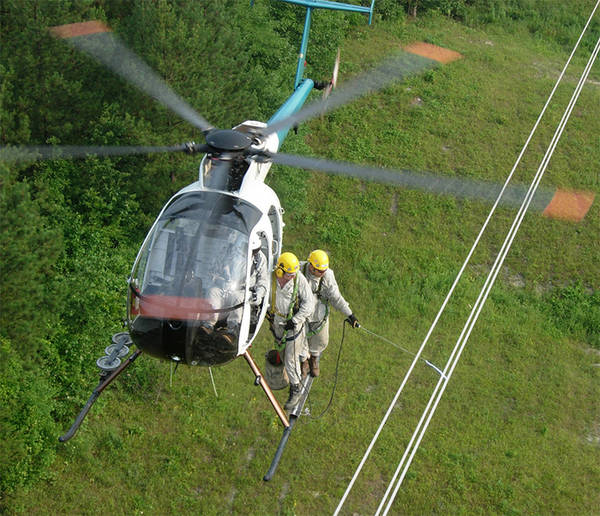
\includegraphics[width=0.6\textwidth]{./insphelic}				
	\caption{Inspeção de linhas de transmissão feita por aeronaves tripuladas.}		
	\label{img:ihelic}												
\end{figure}													
%----------------------------------------------------------
	
%---------------picture------------------------------------
\begin{figure} [h!]												 
	\centering													 
	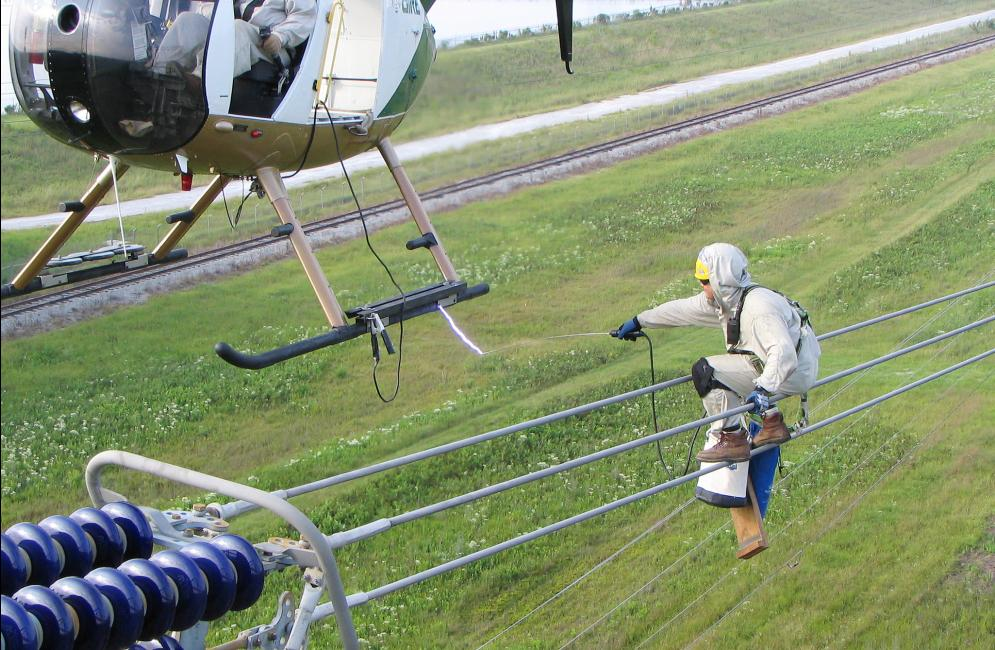
\includegraphics[width=0.6\textwidth]{./insphelichuma}				 
	\caption{Interação humana durante a inspeção de linhas de transmissão.}		
	\label{img:ihelichuma}												 
\end{figure}													 
%----------------------------------------------------------

Em alguns casos, devido às características geográficas da região, condições climáticas e outros fatores que venham a dificultar o sobrevôo, há uma grande exposição dos tripulantes a riscos associados à tarefa. Além dos perigos aos quais os tripulantes são expostos, a inspeção feita com aeronaves tem um custo bastante elevado. Outra forma alternativa de inspeção é o uso de veículos terrestres, porém essa forma é muito limitada, pois boa parte das linhas de transmissão está localizada em áreas de difícil acesso terrestre, muitas vezes restritas pelas características geográficas da região. Além disso, o ângulo de visão é, muitas vezes, desfavorável para a realização da inspeção.

%---------------picture------------------------------------
\begin{figure} [h!]												 
	\centering													 
	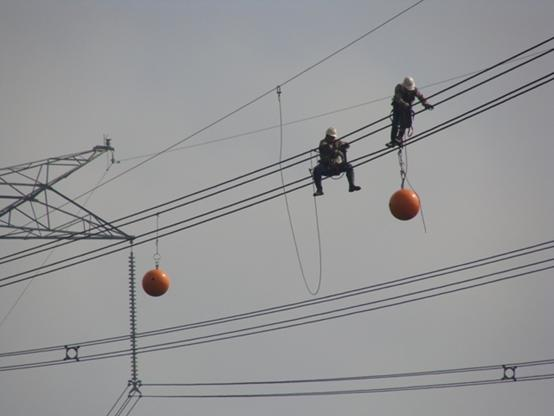
\includegraphics[width=0.6\textwidth]{./insphuma}				 
	\caption{Realização de inspeção em linhas de transmissão através da observação humana.}		
	\label{img:ihuma}												 
\end{figure}													 
%----------------------------------------------------------

Outra maneira de inspecionar as linhas de transmissão é através de eletricistas que literalmente caminham sobre os cabos de linhas de transmissão de alta tensão (Figura \ref{img:ihuma}), realizando inspeção visual e termográfica. Esse tipo de inspeção é lenta e não é viável, tendo em vista que o país possui milhares de quilômetros de linhas de transmissão.

Neste contexto vários robôs de inspeção de linhas de transmissão foram desenvolvidos, porém poucos deles consistiram em projetos de engenharia que sejam aplicáveis no mundo real, além disso a maioria eram robôs tele-operados, ou seja robôs controlados por seres humanos. Um dos pontos diferenciais deste projeto de tese é a proposição de um desenvolvimento de uma navegação autônoma utilizando técnicas de aprendizagem de máquinas até então não utilizadas em robôs de inspeção de linhas de transmissão de alta tensão.

%--------- NEW SECTION ----------------------
\section{Objetivos}
\label{sec:obj}


Nesta se\c{c}\~ao os objetivos principal (tamb\'em
pode-se se utilizar a palavra meta) da monografia de
gradua\c{c}\~ao ou especializa\c{c}\~ao, disserta\c{c}\~ao de
mestrado ou tese de doutorado s\~ao apresentados.


\subsection{Objetivos Específicos}
\label{ssec:objesp}

Nesta se\c{c}\~ao os objetivos espec\'ificos (tamb\'em
pode-se se utilizar a palavra meta) da monografia de
gradua\c{c}\~ao ou especializa\c{c}\~ao, disserta\c{c}\~ao de
mestrado ou tese de doutorado s\~ao apresentados.

%--------- NEW SECTION ----------------------
\section{Justificativa}
\label{sec:justi}

%O pesquisador/estudante deve apresentar os aspectos mais
%relevantes da pesquisa ressaltando os impactos (e.g. cient\'ifico,
%tecnol\'ogico, econ\^omico, social e ambiental) que a pesquisa
%causar\'a. Deve-se ter cuidado com a ingenuidade no momento em que
%os argumentos forem apresentados.

A inspeção de linhas de transmissão de alta tensão é uma tarefa difícil e altamente perigosa, atualmente esta inspeção é realizada através do auxílio de helicópteros os quais percorrem trajetórias próximas às linhas de transmissão e utilizam de câmeras termográficas as quais medem a temperatura nos cabos a partir da associação da quantidade de radiação emitida em determinada faixa de comprimento de onda com uma determinada temperatura. Porém os gastos com este tipo de inspeção são extremamente elevados, como consequência, as empresas responsáveis pela transmissão de energia não monitoram continuamente as condições dos cabos, e realizam inspeções nas linhas de transmissão em intervalos grandes. Outro modo de inspecionar as linhas de transmissão é através de eletricistas que literalmente andam sobre os cabos das linhas de transmissão de alta voltagem fazendo uma inspeção visual e podendo levar algum equipamento para medição de temperatura ao longo da linha, porém este tipo de inspeção é lenta e é inviável verificar milhares de quilômetros de linhas de transmissão utilizando este método.
Ambos os modos de inspeção de linhas de transmissão são arriscados, trazem perigos para as pessoas que estão a bordo do helicóptero; já que, este tem de voar próximo às linhas de transmissão e trazem perigos para o eletricista que irá andar sobre os cabos inspecionando-os visualmente ou com auxílio de algum equipamento, além de desconhecer-se completamente o efeito dos campos eletromagnéticos intensos desta região sobre a saúde destes eletricistas. Como consequência, realizar a inspeção de linhas de transmissão através da utilização de robôs móveis é algo que vem ganhando destaque no século XXI. Isto somente foi possível por causa dos avanços tecnológicos como sistema de localização global, os sistemas de transmissão de informação sem fio, a construção de micro-controladores mais baratos, rápidos e com maior capacidade de processamento, além dos grandes avanços que a computação e a microeletrônica têm obtido. Com isso as tarefas que seres humanos executam em ambientes insalubres, perigosos ou inóspitos poderão ser substituídas por uma mão-de-obra automatizada. Além disso, a aplicação da robótica móvel pode ser utilizada para a redução de custos.  No caso específico deste trabalho, a utilização de robôs de inspeção para linhas de transmissão atende a ambos os aspectos.
Um robô de inspeção de linhas de transmissão deve ser capaz de desviar de obstáculos como grampos de suspensão, grampos terminal passante, emendas a compreensão, emenda total pré-formada, tentos partidos, cabos amassados e dispositivos anti-vibração como amortecedores e festão. Estes obstáculos devem ser transpostos por sequências de movimentos executadas pelo robô. Além disso, idealmente o robô deve apresentar o menor peso, comprimento, altura, ter perfeita aerodinâmica, um formato desprovido de pontas, a maior autonomia possível, baixo custo, além de apresentar uma blindagem eletromagnética que deve impedir que os intensos campos magnéticos e elétricos, devido às elevadas correntes que passam nas linhas de transmissão, danifiquem os componentes eletrônicos, além disso, deve apresentar um sistema de comunicação wireless que não seja influenciado pelo elevado campo eletromagnético ao redor dos cabos, além de apresentar motores com elevado rendimento mecânico e elétrico, não apresentar derrapagem quando o mecanismo para movimentação das rodas for acionado, dentre outros.

Pagnano et. al \cite{pagnano2013roadmap} conclui que uma das principais buscas em futuros projetos devem estar centradas no desenvolvimento de detecção e transposição de obstáculos de forma autônoma, ou seja, não mais atribuir sequências de movimentos para os robôs mas desenvolver algoritmos de controle para que a detecção e ultrapassagem seja realizada de forma autônoma. Outro ponto a se observar é a completa abrangência de autonomia do robô durante sua navegação. 
  
Embora respondam por um número pequeno de ocorrências, se comparadas com as ocorrências em linhas de distribuição, um evento em uma linha de transmissão impacta de maneira desproporcionalmente mais severa, visto que a quantidade de clientes atendidos pelas linhas de transmissão é bem superior ao da linha de distribuição, afinal estas últimas são alimentadas pelas linhas de transmissão.

A manutenção preventiva é o procedimento mais adequado para aumentar a confiabilidade e evitar ocorrências indesejáveis em linhas de transmissão. No entanto, devido ao maior nível de tensão e conseqüentemente de maior escala das estruturas físicas da linha; efetuar a manutenção preventiva de maneira manual é uma tarefa muito difícil, custosa, por vezes requerendo o desligamento da linha. 

O uso de uma ferramenta automatizada para a inspeção destas linhas possibilitará uma redução no número e na freqüência de eventos em linhas de transmissão, aumentando a confiabilidade do sistema elétrico e reduzindo as perdas de energia; contribuindo para a melhoria do processo interno e a qualidade do serviço oferecido ao consumidor final, o que resulta em ganho financeiro para as concessionárias. Além deste benefício, é importante ressaltar que interrupções no fornecimento, mesmo que por curto espaço de tempo, têm como conseqüência impactos negativos sobre a sociedade e sobre a imagem da concessionária, sujeita à exposição na mídia.

Porém, a prática mostra que a idealização de soluções para os problemas levantados é algo distante da realidade, isto porque, além de ser fisicamente impossível de representar-se de forma exata situações ideais na prática; devido às perdas de energia e às inúmeras variáveis que teriam de ser abordadas para representar um problema de forma exata, mesmo que fosse possível construir um modelo muito próximo a realidade, o custo iria ser um dos fatores que iria inviabilizar a escolha dos melhores materiais e dos melhores dispositivos. Assim deve-se observar que, em geral, os robôs devem atender as características conforme certos requisitos de projeto, de modo que se aproxime ao máximo da condição ideal, desde que o custo permaneça abaixo de um valor aceitável. 


%--------- NEW SECTION ----------------------
\section{Requisitos do cliente}
\label{sec:reqc}
asjdflkasjdlfjsdlk;f

%--------- NEW SECTION ----------------------
\section{Organização do \thetypework}
\label{section:organizacao}

Este documento apresenta $x$ capítulos e está estruturado da seguinte forma:

\begin{itemize}

  \item \textbf{Capítulo \ref{chap:intro} - Introdução}: Contextualiza o âmbito, no qual a pesquisa proposta está inserida. Apresenta, portanto, a definição do problema, objetivos e justificativas da pesquisa e como este \thetypeworkthree está estruturado;

  \item \textbf{Capítulo \ref{chap:concep} - Nome do capítulo}: XXX;


  \item \textbf{Capítulo \ref{chap:conc} - Conclusão}: Apresenta as conclusóes, contribuições
  e algumas sugestões de atividades de pesquisa a serem desenvolvidas no futuro.

\end{itemize}

    \chapter{Conceito do Sistema}
\label{chap:concep}

\begin{flushright}
   \begin{list}{}{
      \setlength{\leftmargin}{4.5cm}
      \setlength{\rightmargin}{0cm}
      \setlength{\labelwidth}{0pt}
      \setlength{\labelsep}{\leftmargin}}
      \item Para um robô, o ambiente é um mar de ambiguidades, no qual ele vai afundar ou nadar a depender da robustez de sua percepção.
      \begin{list}{}{
      \setlength{\leftmargin}{0cm}
      \setlength{\rightmargin}{0cm}
      \setlength{\labelwidth}{0pt}
      \setlength{\labelsep}{\leftmargin}}
      \item \cite{Fitzpatrick}
      \end{list}
   \end{list}
\end{flushright}

A percepção é, de acordo com o dicionário \citeonline{perc_michaelis}, a capacidade de distinguir por meio dos sentidos ou da mente.

Segundo \citeonline{chuck}, este é o ponto fraco mais comuns em robôs pois para garantir sua segurança e confiabilidade é necessário que o mesmo tenha a capacidade de interpretar as variáveis ambientais. A percepção é o que torna os robôs diferentes de simples mecanismos, pois é ela quem dá a habilidade de adequar suas operações de acordo com as influências externas.

A percepção do ELIR pode ser definida como um sistema integrado de sensoriamento e com unidades de processamento, em que seus dados serão utilizados como parâmetros de tomada de decisão e disponibilizados durante a operação de inspeção ao operador.

O sistema foi projetado de forma a possuir três subsistemas principais: segurança, georreferenciamento e detecção. A descrição de cada um dos subsistemas e suas funcionalidades serão mostradas nas próximas sessões.



%--------- NEW SECTION ----------------------
\section{Estudo do estado da arte}
\label{sec:sota}
Diante dos desafios apresentados nesta trabalho, faz-se oportuno apresentar os projetos que contribuíram para o desenvolvimento da solução final. De forma muito incipiente os projetos para desenvolvimento de robôs de inspeção em linhas de transmissão, ainda são poucos. \citeonline{pagnano2013roadmap} se propos a descrever um roadmap para o desenvolvimento futuro dos robôs de inspeção em linha de transmissão, reforçando o aspecto da autonomia dos robôs e sua confiabilidade na execução das transposições dos obstáculos.

Como apontado anteriormente através do capítulo inicial deste trabalho, objetiva-se o desenvolvimento de robôs de inspeção no qual utiliza as linhas de transmissão para realizar sua movimentação, neste sentido pode-se observar um dos primeiros trabalhos no desenvolvimento destes robôs apresentado por \citeonline{ventrella2003robo}. Este robô foi desenvolvido para deslocar-se ao longo do cabo de transmissão tendo controle de parada, avanço e retorno via rádio, ou seja tele-operado. O sistema pode gerar imagens do cabo onde são enviadas também via rádio, com isso o operador pode também realizar a transposição dos obstáculos. A Figura \ref{img:roboventrella} apresenta o protótipo do robô, mostrando o seu sistema de locomoção.

%---------------picture------------------------------------
\begin{figure} [h!]	
	\caption{Protótipo do robô desenvolvido por Ventrella et. al.}
	\label{img:roboventrella}											 
	\centering													 
	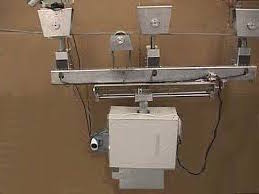
\includegraphics[width=0.5\textwidth]{./roboventrella}
	%\fdireta{ventrella2003robo}			 											 
\end{figure}													 
%----------------------------------------------------------

O conceito de um robô móvel para instalação e remoção autônoma de esferas de sinalização aéreas em linhas de transmissão de energia (Firugar \ref{img:campos}) é apresentado por \citeonline{campos2002mobile}. Segundo os autores, um computador de bordo é responsável pelo controle através dos dados obtidos pelos sensores e dos comandos enviados por um operador de solo. Os comandos do operador são transmitidos por ondas de rádio, o que permite que o sistema seja remotamente operado a uma distância de até 2 km. O equipamento foi testado em campo em uma situação real e mostrou-se eficiente e robusto. De acordo com \citeonline{gonccalves2013review}, apesar do mecanismo proposto por \citeonline{campos2002mobile} não superar obstáculos nem navegar em linhas entre duas torres, é simples e funcional.

%---------------picture------------------------------------
\begin{figure} [h!]	
	\caption{Teste em campo realizado com o robô para instalação e remoção de esferas de sinalização aérea.}
	\label{img:campos}											 
	\centering													 
	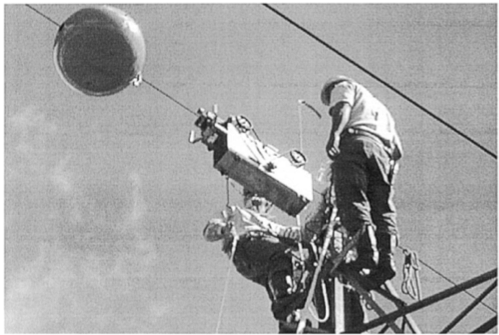
\includegraphics[width=0.6\textwidth]{./campos}
	%\fdireta{campos2002mobile}			 											 
\end{figure}													 
%----------------------------------------------------------

Apoiado pelo financiamento do Plano Nacional Chinês 863, \citeonline{zhou2005control} propuseram um robô (Figura \ref{img:zhou}) capaz de ultrapassar qualquer tipo de obstáculo (até torres) ao trafegar ao longo de uma linha de transmissão de até 110 kV. O robô conta com uma câmera; as imagens de inspeção, por sua vez, são enviadas para uma estação de trabalho do solo através de um sistema de comunicação sem fio.  

%---------------picture------------------------------------
\begin{figure} [h!]	
	\caption{Configuração do robô de inspeção.}
	\label{img:zhou}											 
	\centering													 
	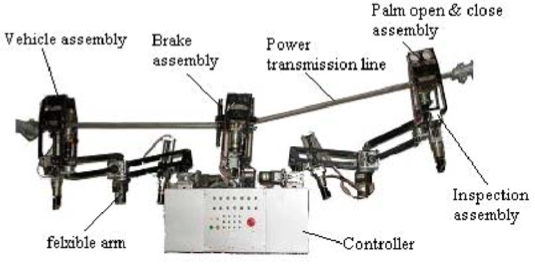
\includegraphics[width=0.6\textwidth]{./zhou}
	%\fdireta{zhou2005control}			 											 
\end{figure}													 
%----------------------------------------------------------

De acordo com a Figura \ref{img:zhou}; a estrutura mecânica do robô desenvolvido por \citeonline{zhou2005control} é composta por cinco grandes partes: mecanismo de movimentação (vehicle driving mechanism); sistema de parada (brake system assembly); braços flexíveis (flexible arms); garras (palm gripper); fonte de alimentação e sistema de controle (power supply and controller). Para assegurar a flexibilidade requerida o robô (que pesa cerca de 45 kg e tem 1,2 m de comprimento) tem 16 eixos de movimentação, podendo vencer inclinações de até 60$^{\circ}$. 

Como parte do programa de pesquisa de \citeonline{montambault2007design} encarregaram-se do desenvolvimento de uma tecnologia para inspeção e manutenção de linhas de transmissão de 735 kV, denominada LineScout (Figura \ref{fig:linescout}). Segundo \citeonline{montambault2007design}, o protótipo deste robô móvel tele operado (pesando 100 kg) foi testado e validado em muitas configurações de linhas e de sequências de obstáculos, sob condições de campo.

%------ picture with two parts -------------
\begin{figure}[h!]
		\caption{Robô LineScout.}
%------ picture part a ---------------------
		\begin{subfigure}[b]{0.5\textwidth}
		  	\centering
		  	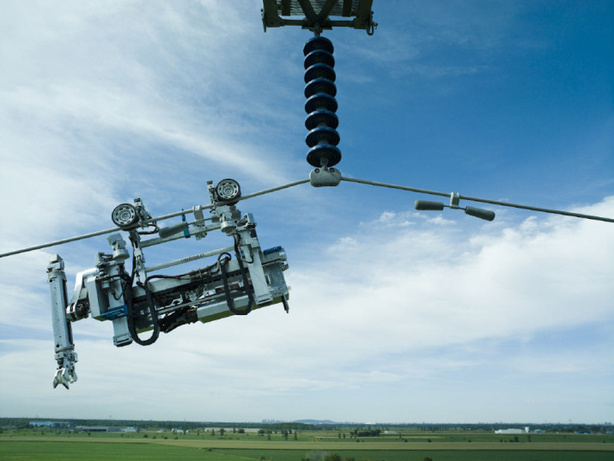
\includegraphics[width=0.85 \textwidth]{./linescout1} 
		  	\caption{robô em operação}
		  	\label{fig:linescout1}
		\end{subfigure} 
%------ picture part a ---------------------
		\begin{subfigure}[b]{0.5\textwidth}
		  	\centering
		  	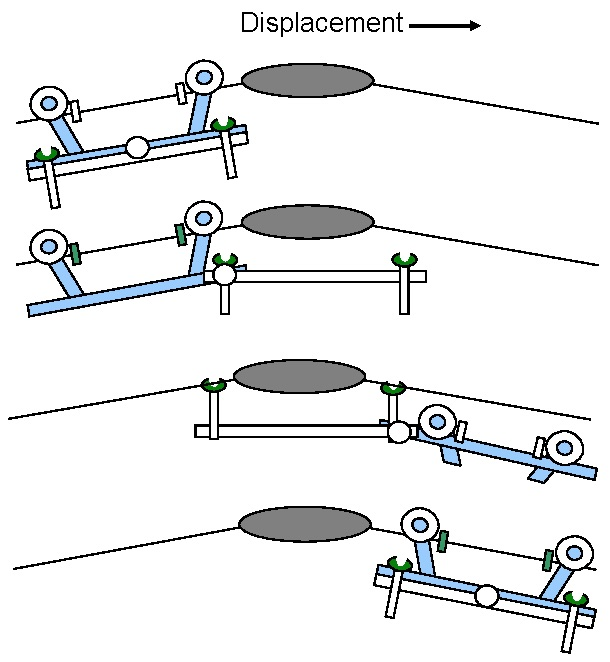
\includegraphics[width=0.55 \textwidth]{./linescout2} 
		  	\caption{esquema de movimentos para ultrapassagem de obstáculos.}
		  	\label{fig:linescout2}
		\end{subfigure} 
%----- info - central picture --------------
	  %\caption{Robô LineScout.} 
	  %\fdireta{montambault2007design} 
	  \label{fig:linescout}
\end{figure}
%-------------------------------------------

O LineScout, como mostrado na Figura \ref{fig:linescout}, utiliza o cabo condutor como suporte; o uso de rodas para movimentação não só possibilita a locomoção rápida e eficiente ao longo da linha, como também permite passar por cima de alguns obstáculos. Para ultrapassar outros tipos de obstáculos é empregada a sequência de movimentos esquematizados na Figura \ref{fig:linescout2}.
Em 2008 \citeonline{katrasnik2010climbing} propuseram um conceito híbrido para inspeção de linhas de transmissão; o qual combina o uso de um veículo aéreo não tripulado (VANT) e um robô móvel (Figura \ref{img:katrasnik}). Em seus estudos conceituais os autores comparam os três tipos de sistemas para inspeção: os robôs móveis, os por veículos aéreos e os híbridos; concluindo que, apesar da baixa qualidade de inspeção e autonomia, o sistema proposto tem como vantagem a universalidade e a facilidade de projeto. \citeonline{katrasnik2010climbing} acreditam ainda que a solução híbrida provavelmente não terá a autonomia de superação de obstáculos possíveis aos robôs móveis tendo, porém, um provável custo menor de desenvolvimento.  

%---------------picture------------------------------------
\begin{figure}[h!]	
	\caption{Robô híbrido e seus componentes.}
	\label{img:katrasnik}											 
	\centering													 
	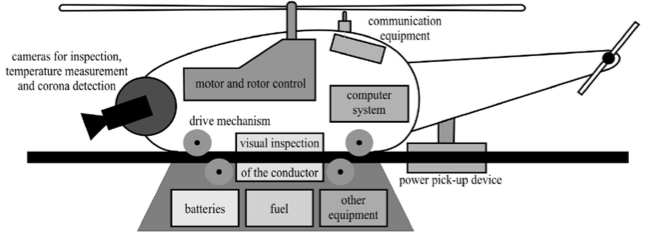
\includegraphics[width=0.8\textwidth]{./katrasnik}
	%\fdireta{katrasnik2010climbing}			 											 
\end{figure}													 
%----------------------------------------------------------

Os primeiros estágios de desenvolvimento do Expliner (Figura \ref{img:expliner1}) são apresentados no artigo de \citeonline{debenest2008expliner}. Este robô tele operado foi projetado para realização de manutenção preventiva de linhas de transmissão de alta-voltagem e conta com dois pontos de apoio e um contrapeso.  A movimentação do contrapeso permite que haja o controle da posição do centro de massa e o consequente levantamento em um dos pontos de suporte; este mecanismo possibilita a ultrapassagem de obstáculo (a exemplo do mostrado na Figura \ref{img:expliner2}).

%------ picture with two parts -------------
\begin{figure}[h!]
		\caption{Robô Expliner.}
%------ picture part a ---------------------
		\begin{subfigure}[b]{0.5\textwidth}
		  	\centering
		  	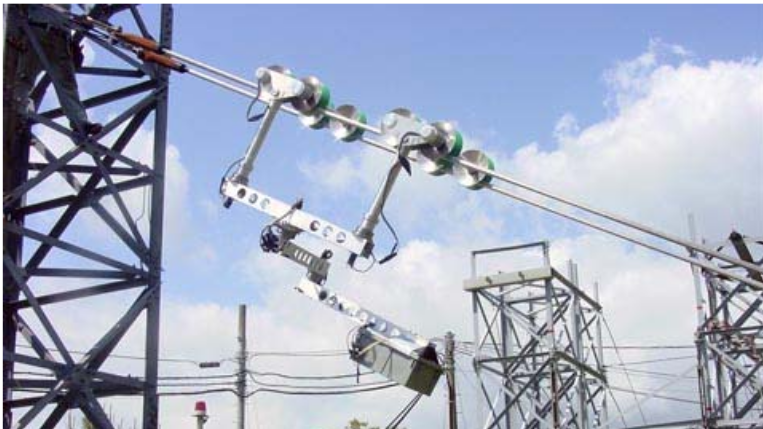
\includegraphics[width=0.9 \textwidth]{./expliner} 
		  	\caption{robô e sua submontagens.}
		  	\label{img:expliner1}
		\end{subfigure}
%------ picture part a ---------------------
		\begin{subfigure}[b]{0.5\textwidth}
		  	\centering
		  	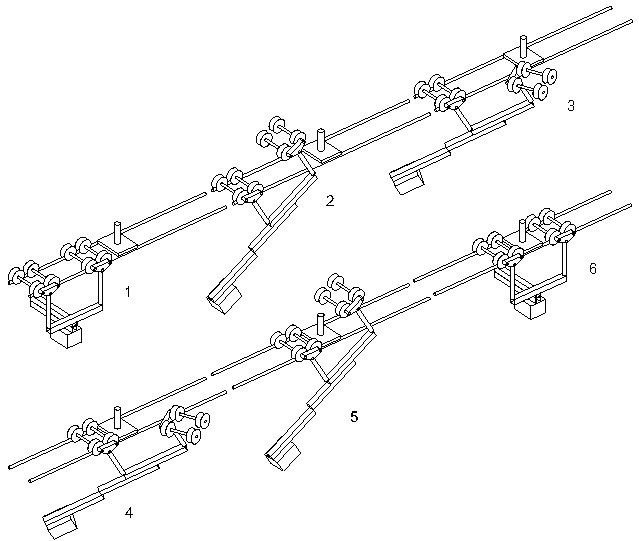
\includegraphics[width=0.6 \textwidth]{./expliner2} 
		  	\caption{esquema de movimentos para ultrapassagem de obstáculos.}
		  	\label{img:expliner2}
		\end{subfigure} 
%----- info - central picture --------------
	  %\caption{Robô Expliner.} 
	  %\fdireta{debenest2008expliner} 
	  \label{img:expliner}
\end{figure}
%-------------------------------------------

De acordo com \citeonline{debenest2008expliner}, o Expliner pode ser semi-controlado através de um sistema de comunicação sem fio, ou seja, o usuário está sempre encarregado da sua operação não precisando, porém, controlar todos os detalhes, mas sim autorizar a realização de tarefas pré-programada; as sequências de movimento ficam gravadas na sua memória. Por pesar 84 kg, um cabo de acesso deve ser usado para colocar o robô na linha de transmissão.  De acordo com os autores, os testes realizados mostram que o Expliner pode mover-se até m/min e superar inclinações de até 30 graus. 

Já a proposta de \citeonline{rangel2009sistema} é o desenvolvimento de uma plataforma de monitoramento aéreo a ser utilizado para inspecionar linhas de alta voltagem. Para tal, a integridade da linha é verificada com o auxílio de um VANT (Figura \ref{img:rangel2}), onde é instaladas câmeras de vídeo, equipamentos de controle e de telemetria. O VANT é pilotado remotamente por um operador que se encontra na estação de solo (Figura \ref{img:rangel2}). As imagens capturadas e os dados georreferenciados da linha e do terreno são enviados, em tempo real, ao solo para posterior armazenamento e processamento.

%---------------picture------------------------------------
\begin{figure} [h!]	
	\caption{VANTs utilizados como plataforma de testes.}
	\label{img:rangel1}											 
	\centering													 
	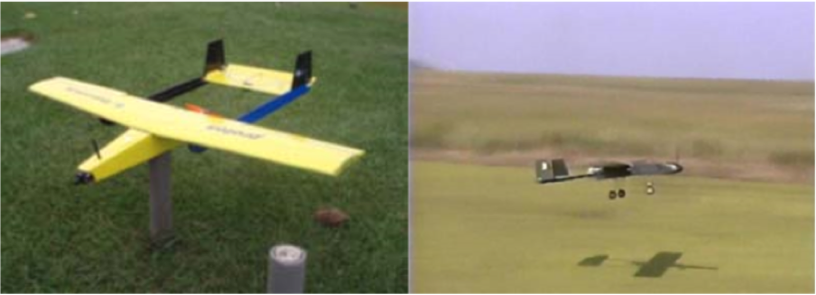
\includegraphics[width=0.6\textwidth]{./rangel}
	%\fdireta{rangel2009sistema}			 											 
\end{figure}													 
%----------------------------------------------------------

%---------------picture------------------------------------
\begin{figure} [h!]	
	\caption{Sistema de monitoramento aéreo para linhas de transmissão de energia.}
	\label{img:rangel2}											 
	\centering													 
	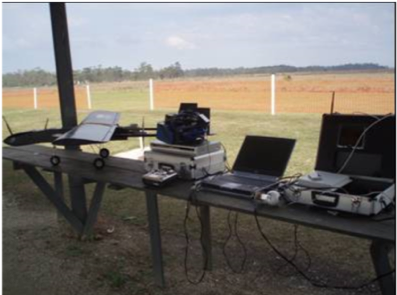
\includegraphics[width=0.6\textwidth]{./rangel2}
	%\fdireta{rangel2009sistema}			 											 
\end{figure}													 
%----------------------------------------------------------

Durante a pesquisa da inspeção utilizando VANTs, foi constatado que estes não substituem com plenitude as aeronaves tripuladas nesta tarefa, uma vez que existem limitações quanto à proximidade dos veículos com a linha de transmissão para que não haja interferência eletromagnética no sistema. Os autores citam ainda, que esta proposta presta-se, fundamentalmente, a identificação e diagnóstico do problema, não sendo possível a realização de manutenção corretiva (como ocorre quando há a inspeção por helicóptero tripulado).  
\citeonline{li2010autonomous} em seu trabalho descrevem o desenvolvimento de um robô móvel para inspeção de linhas de transmissão de 500 kV capaz de superar alguns obstáculos como contrapesos, torre de ancoragem, e torres de torção (Figura \ref{img:li}). O robô projetado conta com treze motores e tem sua mobilização, inspirada no comportamento dos macacos. Estruturado em um mecanismo formado por engrenagens sem-fim, rodas, garras, parafusos e porcas ele tem capacidade para escalar linhas com no máximo 60 graus. O protótipo deste robô, (com 30 kg e tem 1,2 m de comprimento e 0,8 m de altura) ainda está em fase de desenvolvimento e carece de uma maior robustez para a efetiva realização de algumas inspeções necessárias para uma boa manutenção preventiva das linhas de transmissão.

%---------------picture------------------------------------
\begin{figure} [h!]	
	\caption{Teste do robô de inspeção.}
	\label{img:li}											 
	\centering													 
	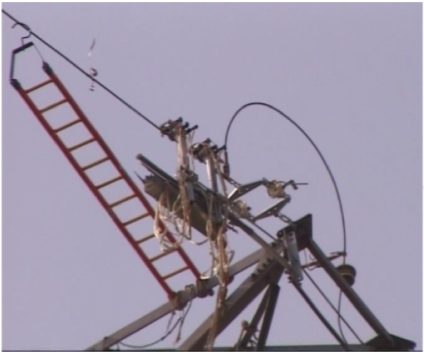
\includegraphics[width=0.6\textwidth]{./li}
	%\fdireta{li2010autonomous}			 											 
\end{figure}													 
%----------------------------------------------------------

O robô proposto por \citeonline{wang2010design} apresentam um mecanismo diferenciado para a realização da inspeção de linhas de transmissão. Como pode ser observado na Figura \ref{img:wang}, este robô móvel conta com uma estrutura bípede e os seus dois pés podem ser presos à linha de transmissão; os seus ciclos de movimento sob a linha são compostos por fases onde há um único apoio e outras fases onde há dois apoios. Cada perna tem uma junta prismática que permite que o seu tamanho seja ajustado fazendo com que o seu centróide sempre coincida com o eixo da articulação central (hip joint), reduzindo o consumo de energia e mantendo a sua estabilidade na quando o robô está mono apoiado. 

%---------------picture------------------------------------
\begin{figure} [h!]	
	\caption{Modelo 3D do robô bípede para inspeção de linhas de transmissão.}
	\label{img:wang}											 
	\centering													 
	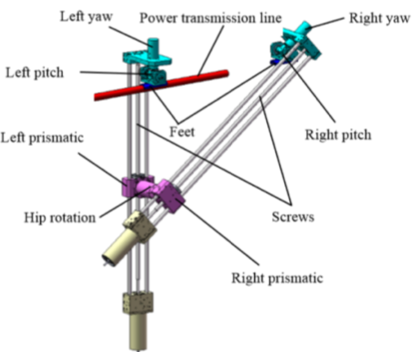
\includegraphics[width=0.6\textwidth]{./wang}
	%\fdireta{wang2010design}			 											 
\end{figure}													 
%----------------------------------------------------------

O protótipo do robô apresentado por \citeonline{wang2010design} possui 800 mm de altura e 100 mm de largura, quando todas as juntas estão na posição zero; o maior obstáculo que pode transpor tem 300 mm de comprimento. Os autores concluem que os próximos trabalhos a serem realizados com este protótipo devem focar na inclusão de sensor de detecção de linha, controle on-board e testes em ambientes reais de linha de transmissão e obstáculos.  
O “Cable Crawler” é tratado por \citeonline{buhringer2010cable}, um robô tele operado para inspeção de linha de transmissão de alta voltagem que trafega ao longo do cabo terra. Este robô, que pesa 53 kg, conta com um mecanismo que permite com que ele transponha desde pequenos obstáculos até as torres (como mostrado na Figura 18). 

%---------------picture------------------------------------
\begin{figure} [h!]	
	\caption{Demonstração da sequência de movimentos do Cable Crawler ultrapassando uma torre.}
	\label{img:buehringer}											 
	\centering													 
	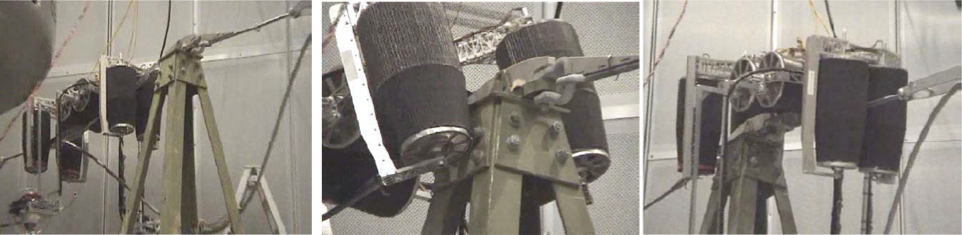
\includegraphics[width=0.6\textwidth]{./buehringer}
	%\fdireta{buhringer2010cable}			 											 
\end{figure}													 
%----------------------------------------------------------

Gonçalves e Carvalho em seus trabalhos \cite{goncalves2010graphical} e \cite{gonccalves2013review}  apresentam os resultados dos estudos desenvolvidos a cerca de um robô móvel suspenso por fio projetado para manutenção e inspeção de linhas de energia e/ou telecomunicação. Segundo \citeonline{gonccalves2006kinematics} este robô, de fácil controle, tem a capacidade de transpor alguns obstáculos, como por exemplo grampos e esferas de sinalização, independentemente de sua posição; uma vez que é dotado de quatro pernas de comprimentos variáveis.

%---------------picture------------------------------------
\begin{figure} [h!]	
	\caption{Configuração geral do robô suspenso por fio com pernas iguais.}
	\label{img:goncalves}											 
	\centering													 
	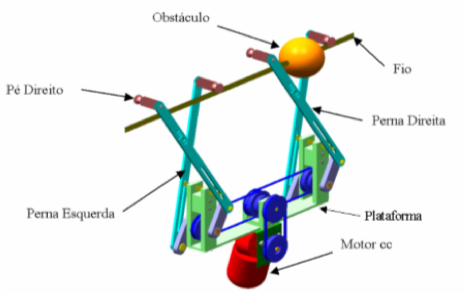
\includegraphics[width=0.6\textwidth]{./goncalves}
	%\fdireta{gonccalves2006kinematics}			 											 
\end{figure}													 
%----------------------------------------------------------

A Figura \ref{img:goncalves} ilustra a configuração geral do robô proposto por \citeonline{gonccalves2006kinematics} e \citeonline{goncalves2010graphical}. Um dos princípios do seu desenvolvimento é a  facilidade de controle, para tal, a movimentação das quatro pernas é sincronizada por um conjunto de polias e correias acionado por um único motor. 
O Instituto Coreano de Pesquisa em Energia Elétrica propõe, através do trabalho de \citeonline{lee2011development}, um robô para inspeção de luvas de emenda de linhas de transmissão pela medição do campo magnético. O seu programa de interface com o usuário (remoto) mostra a condição da ferramenta, permitindo com que o operador comande os movimentos do robô; além de calcular e apresentar o grau de excentricidade da luva.  

%---------------picture------------------------------------
\begin{figure} [h!]	
	\caption{Equipamento para inspeção de luvas de emendas de linhas de transmissão.}
	\label{img:lee}											 
	\centering													 
	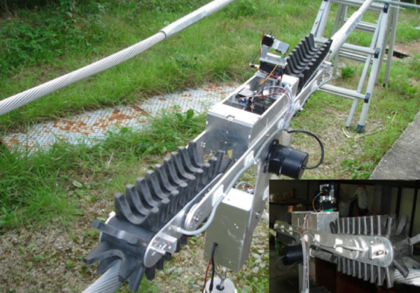
\includegraphics[width=0.6\textwidth]{./lee}
	%\fdireta{lee2011development}			 											 
\end{figure}													 
%----------------------------------------------------------

Como pode ser visto na Figura \ref{img:lee}, a estrutura do robô para inspeção de luvas de emendas é formada de duas partes: uma responsável pelo movimento e outra pela inspeção. De acordo com \citeonline{gonccalves2013review}, seu deslocamento assemelha-se a uma lagarta, onde há aderência e locomoção ao longo do cabe através de um sistema de sulcos e ranhuras que permite que o robô supere elevações e depressões sem cair.

\citeonline{phillips2012autonomous} apresentaram em seu trabalho o robô que autonomamente inspeciona linhas de transmissão de alta voltagem desenvolvido pelo Electric Power Research Institute (EPRI); denominado Ti. No campo, este robô é instalado permanentemente à linha de transmissão e é capaz de transpor os obstáculos através de sistemas de by-pass, também permanentes. O Ti dispõe de câmeras de alta definição, câmaras espectro de infravermelho, detectores de interferência eletromagnética e diversos sensores de radiofrequência; os autores acreditam que, desta maneira, o sistema será capaz de fornecer informações completas, precisas e úteis para otimizar a manutenção de linha e melhorar a confiabilidade da transmissão. 

%---------------picture------------------------------------
\begin{figure} [h!]	
	\caption{Robô Ti em teste.}
	\label{img:phillip}											 
	\centering													 
	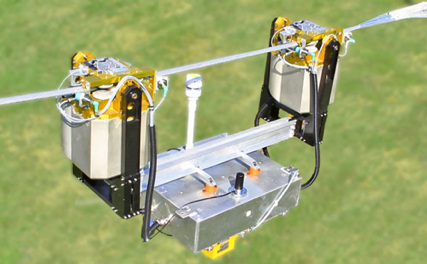
\includegraphics[width=0.6\textwidth]{./phillip}
	%\fdireta{phillips2012autonomous}			 											 
\end{figure}													 
%----------------------------------------------------------

Baseado na proposta de \citeonline{katrasnik2010climbing}, \citeonline{gonccalves2013review} expõem seus estudos a cerca da ideia de um robô modular (Figura \ref{img:goncalvesecarvalho}). Nesta solução cada módulo possuirá sua própria movimentação, função e sistema de energia, podendo transitar ao longo do cabo de alta voltagem ou do de terra. O primeiro módulo carregará um UAV, veículo que será responsável pelo carregamento de todos os módulos no momento da ultrapassagem de obstáculos, podendo ser tele operado. Existirá ainda, o módulo incumbido da troca de baterias dos demais. 

%---------------picture------------------------------------
\begin{figure} [h!]	
	\caption{Robô modular.}
	\label{img:goncalvesecarvalho}											 
	\centering													 
	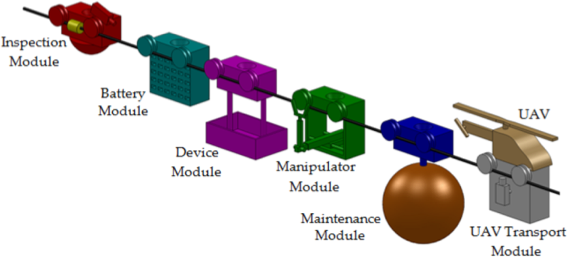
\includegraphics[width=0.6\textwidth]{./goncalvesecarvalho}
	%\fdireta{gonccalves2013review}			 											 
\end{figure}													 
%----------------------------------------------------------

\citeonline{gonccalves2013review} acreditam que, uma vez que cada módulo possuirá uma finalidade específica, haverá a otimização do seu peso total (dependendo da atividade) reduzindo o consumo de energia. Os autores afirmam, ainda, diante da individualidade dos módulos, que o robô poderá ser projetado para diversas tarefas (inspeção, manutenção, instalação, limpeza, captura de imagens, etc.) sem necessariamente ser pesado e grande (como seria um robô monobloco multitarefa). 

%------

Destacaremos no presente trabalho o robô autônomo apresentado por \citeonline{iirobo} e \citeonline{mourao2015robolinhas} denominado PIRO (Powerlines Inspection Robot) ou D311, fruto da parceria entre CEMIG, SENAI-CIMATEC/BIR (Brazilian Institute of Robotics) e Universidade Federal de Minas Gerais (no âmbito do Programa de Pesquisa e Desenvolvimento Tecnológico do Setor de Energia Elétrica regulado pela ANEEL). 

%---------------picture------------------------------------
\begin{figure} [h!]	
	\caption{Esboço inicial do PIRO.}
	\label{img:piro}											 
	\centering													 
	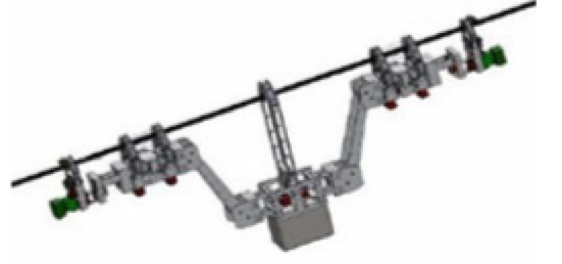
\includegraphics[width=0.6\textwidth]{./piro}
	%\fdireta{iirobo}			 											 
\end{figure}													 
%----------------------------------------------------------

De acordo com os autores, o projeto do PIRO tem como objetivo ser uma proposta inovadora diante dos resultados encontrados anteriormente por outros pesquisadores; sendo autônomo para a realização de inspeção visual e térmica de cabos de transmissão de linhas energizados e transposição automatizada de obstáculos. Para tanto se considerou como pré-requisitos que o robô deve:

\begin{itemize}
	\item Trabalhar em uma faixa de tensão entre 124,2 kV e 151,8 kV com corrente trifásica de 500 A.
	\item Ser autônomo, dependendo de operadores apenas para sua instalação e remoção no trecho a ser inspecionado ou por eventuais paradas emergenciais.
	\item Operar em um cabo condutor LINNET, com diâmetro de 18,3 mm.
	\item Ter massa menor ou igual a 14 kg, permitindo a instalação em campo com a utilização de hastes por apenas dois operadores. 
	\item Ser provido de blindagem elétrica e magnética de forma a assegurar seu funcionamento na linha de transmissão, ou seja, que não haja danos nos seus componentes devido aos campos eletromagnéticos intensos.
	\item Ser capaz de transportar sensores e equipamentos para inspeção visual e térmica, diagnosticando possíveis falhas no sistema que podem interferir no fornecimento de energia elétrica.
\end{itemize}

\citeonline{iirobo} e \citeonline{mourao2015robolinhas} afirmam que o mecanismo do D311 para superação de obstáculo foi inspirado no movimento na lagarta Caterpillar (Figura \ref{img:dubois} ). De acordo com a Figura \ref{img:piro2} , optou-se, ainda, por uma estrutura mecânica modular composta por: Braços, os quais unem a unidade de tração e de apoio. O módulo de tração, responsável pela força motora. Unidade de apoio, a qual atua como ponto de referência do equipamento e funciona como mais um ponto de suporte durante a rotina de ultrapassagem de obstáculos. 

%---------------picture------------------------------------
\begin{figure} [h!]	
	\caption{Movimento da lagarta Caterpillar.}
	\label{img:dubois}											 
	\centering													 
	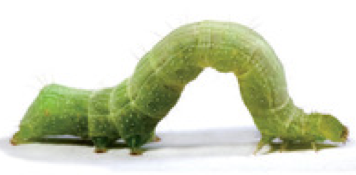
\includegraphics[width=0.6\textwidth]{./dubois}
	%\fdireta{dubois2010complex}			 											 
\end{figure}													 
%----------------------------------------------------------

%---------------picture------------------------------------
\begin{figure} [h!]	
	\caption{Configuração básica da segunda versão do robô PIRO.}
	\label{img:piro2}											 
	\centering													 
	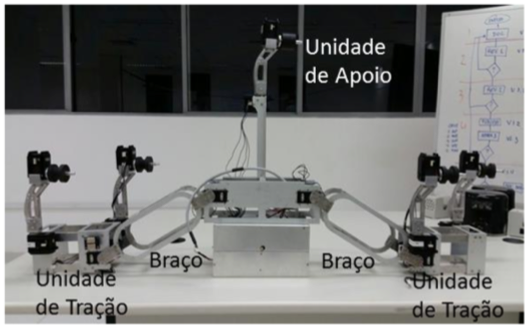
\includegraphics[width=0.6\textwidth]{./piro2}
	%\fdireta{mourao2015robolinhas}			 											 
\end{figure}													 
%----------------------------------------------------------

O PIRO conta com uma estrutura simétrica, que o permite deslocar em ambos os sentidos sem que haja a necessidade de desacoplamento do robô; além de quatro articulações, que provém o número de GDLs necessários seu funcionamento adequado. Sua estrutura é fabricada através de perfis metalon de liga alumínio 2024-T6, o que garantiu redução de tempo de produção, custo e, principalmente, peso. Os autores acreditam que, uma vez que o braço do PIRO tem apenas 153 g e toda a estrutura mecânica tem 1,8 kg; alcançou-se uma inovação ímpar ao estado-da-arte, a massa total da estrutura final do robô é 8,92 kg.
\citeonline{mourao2015robolinhas}, durante os testes realizados em laboratório foi constatado: que a morfologia do robô permite que a transposição de obstáculo; que o sistema de acionamento responde de forma precisa aos comandos de deslocamento, velocidade e aceleração além da rapidez e eficácia do sistema de sensoriamento e visualização. Já os testes executado em linha viva de 138 kV, para verificação quanto à susceptibilidade às interferências eletromagnéticas, sendo que os resultados mostram-se satisfatórios. 
O artigo de \citeonline{iirobo} traz, ainda, um estudo comparativo entre o D311 e outros robôs para inspeção de linhas de alta tensão. Em relação ao LineScout, apresentado por \citeonline{montambault2007design} , o PIRO tem a vantagem de ser autônomo (e não tele operado), ou seja, não depende da habilidade do operador; além de ter massa sete vezes menor, permitindo o seu acoplamento manual. A utilização dos VANTs, por sua vez, apesar da sua maior velocidade de inspeção, em comparação com o D311 apresenta as desvantagens da necessidade de extensa área para pouso e decolagem, menor exatidão na localização dos defeitos, grande influência de perturbações externas e taxas de amostragem insuficientes para elevadas velocidades de varredura.

%--------- NEW SECTION ----------------------
\section{Descrição do sistema robótico}
\label{sec:desc}
As concessionárias de energia elétrica e diversas instituições de pesquisa, nos últimos anos vêm trabalhando na busca de uma solução para a inspeção de linhas de transmissão de alta tensão. A abrangência de suas pesquisas perfazem em grande parte no desenvolvimento de robôs para realizar a inspeção. 
Esta trabalho tomou como base o sistema mecânico desenvolvido no projeto do primeiro robô de inspeção de linha de transmissão brasileiro de baixo peso, apresentado no VII Congresso de Inovação Tecnológica em Energia Elétrica \cite{mourao2015robolinhas}.
A escolha no uso desta solução mecânica originou-se dos resultados alcançados por este projeto diante dos desafios de uma inspeção de linhas de transmissão. Denominado projeto D311 e sob o código Aneel PD-4950-0311/2011, teve como objetivo desenvolver um robô autônomo para executar a inspeção visual e térmica de linhas de transmissão de alta tensão (138kV), realizando automaticamente a transposição de obstáculos presentes na linha de transmissão.
Apesar de alcançar os objetivos inicialmente traçados, o sistema de navegação do robô não era autônomo, seu deslocamento e transposição era baseado em reconhecimentos de padrões e todos os algoritmos pré-estabelecidos eram acionados quando do reconhecimento do padrão.

Diante da ideia estabelecida, esta trabalho promoveu algumas modificações nas estruturas mecânicas para simplificar as modelagens necessárias para a simulação, logo em termos estruturais e dimensionais a estrutura mecânica proposta apresenta modificações consideráveis em relação ao robô do Projeto D311. Para dar suporte a compreensão deste modelo proposto, os desenhos mecânicos desenvolvidos são apresentados no Apêndice \ref{Append:diagmec}. Uma das principais diferenças entre a proposta do robô desta trabalho e do PIRO apresentado por \citeonline{mourao2015robolinhas}, está no fato deste realizar a detecção e classificação de objetos de forma autônoma, além de desempenhar autonomamente as funções de translação e transposição. Outro ponto a ser considerado é a sua flexibilidade em transpor obstáculos, o robô em questão terá uma capacidade de desempenho maior do que o apresentado por \cite{mourao2015robolinhas}; quanto a sua montagem, o robô apresenta simplicidades na fabricação das peças além de possibilidade um número maior de graus de liberdade necessárias para os movimentos. A proposta para o robô é apresentada na figura \ref{img:elir}.

%---------------picture------------------------------------
\begin{figure} [h!]	
	\caption{Protótipo do robô ELIR.}
	\label{img:elir}											 
	\centering													 
	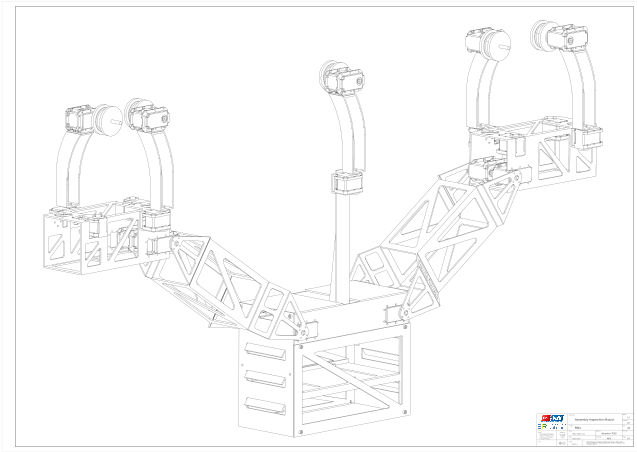
\includegraphics[width=0.7\textwidth]{./elir}
	%\fautor			 											 
\end{figure}													 
%----------------------------------------------------------

Este protótipo será referenciado como robô ELIR, o qual recebe este nome devido a sua representação de Robô de Inspeção Elétrica em inglês, ou seja Electrical Inspection Robot. O ELIR é composto por duas unidades de tração, dois "braços", e uma unidade central. A unidade de tração é composta por um par de garras, com um servomotor e uma roda em cada uma, além disso a estrutura principal da unidade é composta por mais dois servomotores com o objetivo de deslocar as garras da unidade. Os braços são compostos por uma estrutura metálica em alumínio, na extremidade de cada um deles há uma junta de movimentação composta por dois servomotores. A unidade central é onde o processamento do robô se encontra, a unidade também agrega o subsistema de potência do robô.

A proposta do sistema mecânico aqui apresentada foi estudada e simulada por \citeonline{sartori2018}, que diante do dimensional sugerido pela Figura \ref{img:vistaselir} realizou uma análise geométrica do referido sistema robótico ELIR, chegando a conclusão de que não havia interferência mecânica entre a estrutura do robô e os obstáculos durante o processo de movimentação ou de transposição.

%---------------picture------------------------------------
\begin{figure} [h!]	
	\caption{Vista frontal e laterial do robô ELIR.}
	\label{img:vistaselir}											 
	\centering													 
	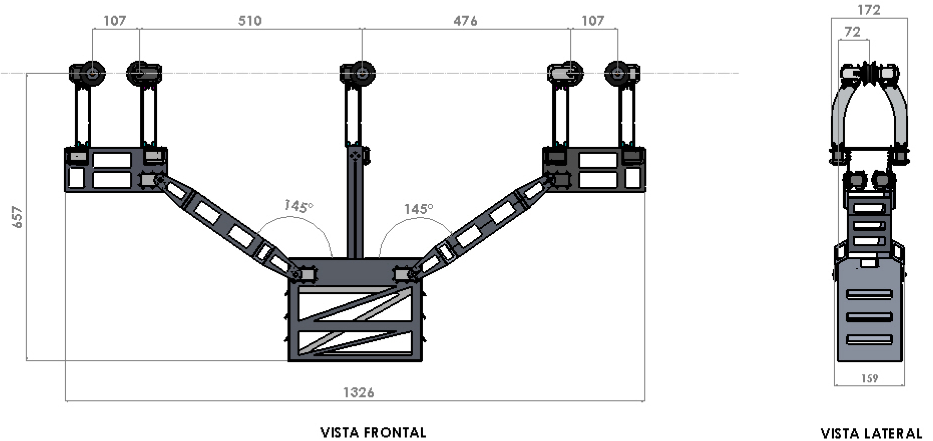
\includegraphics[width=0.7\textwidth]{./vistaselir}
	%\fautor			 											 
\end{figure}													 
%----------------------------------------------------------

 De forma resumida, os dimensionais do sistema robótico é apresentado na Figura \ref{img:vistaselir} e tomando como referência a Figura \ref{img:esquemaelir} juntamente com seus parâmetros e matrizes de transformação, chega-se a conclusão que há uma simetria na geometria do robô ELIR, bastando dessa forma permutar entre a base e o efetuador, ou seja as matrizes da cinemática direta são válidas para as duas extremidades.

%---------------picture------------------------------------
\begin{figure} [h!]	
	\caption{Esquema do ELIR  com os sistemas de coordenadas das suas articulações, para a verificação do deslocamento das roldanas das unidades de tração.}
	\label{img:esquemaelir}											 
	\centering													 
	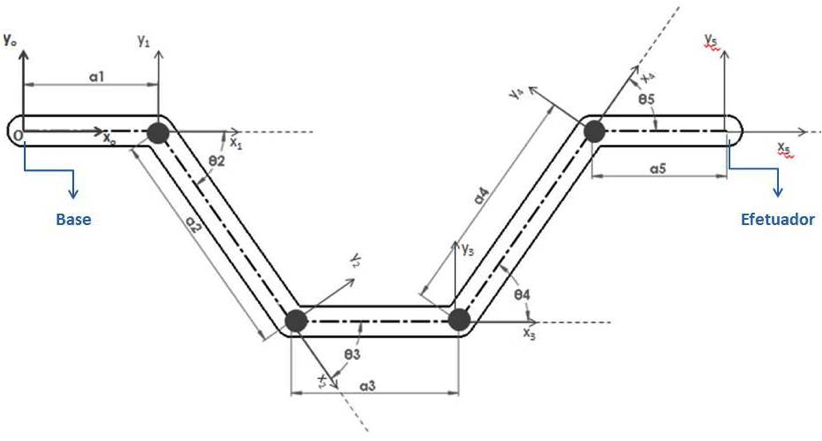
\includegraphics[width=0.7\textwidth]{./esquemaelir}
	%\fautor			 											 
\end{figure}													 
%----------------------------------------------------------

Consequentemente, tomando o sistema e dividindo-o em cinco partes, as matrizes homogêneas do robô são estabelecidas, levando em consideração os parâmetros de Denavit-Hartenberg apresentado na Tabela \ref{tab:parametrodhelir} para o robô ELIR, no qual chega-se aos valores dimensionais dos ângulos de cada junta (Figura \ref{img:esquemaelirdim}) obtidos na análise cinemática.

%----------------table-------------------------------------
\begin{table}[htb!]
	\caption{Parâmetros de DH do ELIR , para a verificação do deslocamento das roldanas das unidades de tração}
	\label{tab:parametrodhelir}
	\centering
	%\begin{tabularx}{\textwidth}{X|l|r|r|r} \hline
	\begin{tabular}{c|c|c|c|c}
		Junta    & ai & di & $\alpha i$ & $\theta  i$ \\ \hline
		1        & a1 & 0  & 0        & $\theta 1$  \\
		2        & a2 & 0  & 0        & $\theta 2$  \\
		3        & a3 & 0  & 0        & $\theta 3$  \\
		4        & a4 & 0  & 0        & $\theta 4$  \\
		5        & a5 & 0  & 0        & $\theta 5$  \\ \hline
	\end{tabular}
	%\fdireta{sartori2018}
\end{table}
%----------------------------------------------------------

%---------------picture------------------------------------
\begin{figure} [h!]	
	\caption{Configuração de juntas, ângulos e links para validação da matriz homogênea obtida na ánalise cinemática.}
	\label{img:esquemaelirdim}											 
	\centering													 
	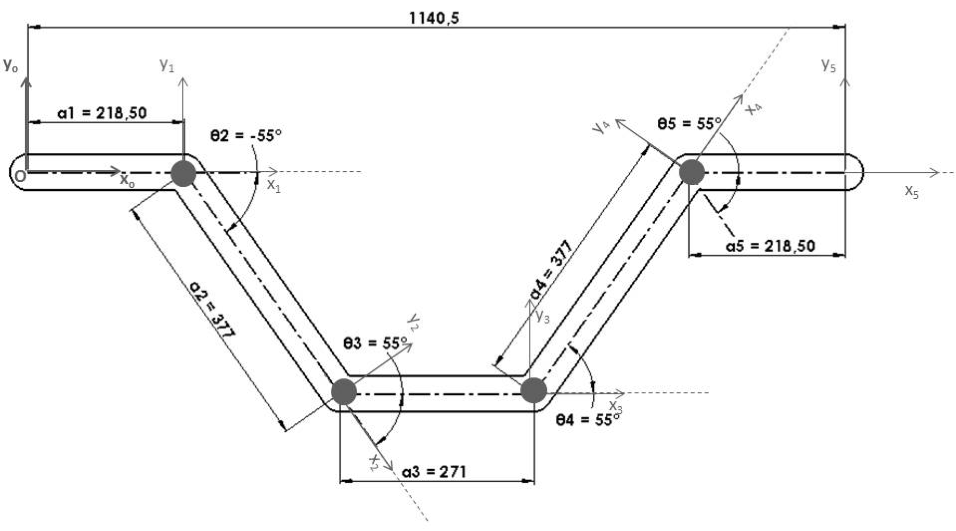
\includegraphics[width=0.9\textwidth]{./esquemaelirdim}
	%\fautor			 											 
\end{figure}													 
%----------------------------------------------------------

A matriz homogênea de cada parte é dada pela Equação \ref{eq:mathomog}. 

%---------------equation-----------------------------------
\begin{equation}
\label{eq:mathomog}
	{A}_{n-1}^{n}=\left (
	\begin{matrix}
 		\cos{\theta}_{n} & -\sin{\theta}_{n} & 0 & {a}_{n}\cos{\theta}_{n} \\ 
 		\sin{\theta}_{n} & \cos{\theta}_{n} & 0 & {a}_{n}\sin{\theta}_{n} \\ 
		0 & 0 & 1 & 0 \\
		0 & 0 & 0 & 1
	\end{matrix}
\right )
\end{equation}
%----------------------------------------------------------

Logo levando-se em consideração que o efetuador do robô esteja numa extremidade, tem-se a matriz transformação homogênea da base definida pela expressão \ref{eq:mathomogbase}.

%4.2
%---------------equation-----------------------------------
\begin{equation}
\label{eq:mathomogbase}
	{A}_{0}^{5}={A}_{0}^{1}\cdot {A}_{1}^{2}\cdot{A}_{2}^{3}\cdot {A}_{3}^{4}\cdot{A}_{4}^{5}=\left (
	\begin{matrix}
 		{r}_{1,1} & {r}_{1,2} & {r}_{1,3} & {x}_{0}^{5} \\ 
 		{r}_{2,1} & {r}_{2,2} & {r}_{2,3} & {y}_{0}^{5} \\ 
 		{r}_{3,1} & {r}_{3,2} & {r}_{3,3} & {z}_{0}^{5} \\
 		0 & 0 & 0 & 1
	\end{matrix}
\right )		
\end{equation}
%----------------------------------------------------------
 
Os elementos da matriz apresentada pela equação \ref{eq:mathomogbase}, são definidos por \citeonline{sartori2018} e serão tomados como parâmetros para esta pesquisa, diante disso chega-se aos dimenstionais apbraesentados na Figura \ref{img:esquemaelirdim} com seus respectivos valores de ângulos, logo podemos encontrar o resultado numérico para a Equação \ref{eq:mathomognum}.

%4.3
%---------------equation-----------------------------------
\begin{equation}
\label{eq:mathomognum}
	{A}_{0}^{5}=\left (
	\begin{matrix}
 		1 & 0 & 0 & 1140.5 \\ 
 		0 & 1 & 0 & 0 \\ 
 		0 & 0 & 1 & 0 \\
 		0 & 0 & 0 & 1
	\end{matrix}
\right )	
\end{equation}
%----------------------------------------------------------

Com isto, pode-se definir qualquer posição do efetuador no espaço de trabalho considerado, assim como identificar as limitações do robô para os movimentos requeridos. Estas definições serão úteis para a elaboração da simulação pretendida nesta trabalho.

Vale ressaltar que toda estruturação metálica, com seus dimensionais são apresentados ao final da trabalho na seção Apêndice, mais especificamente no Apêndice \ref{Append:diagmec}. Um outro ponto importante a se destacar, é que a análise cinemática inversa analisada e simulada por \citeonline{sartori2018} não foi considerada para o desenvolvimento deste trabalho, em subistituição a modelagem matemática será adotado o software \textit{MoveIt!} para estabelecer os posicionamentos das juntas para a realização de uma determinada estratégia a qual se queira desenvolver.

Baseado no conceito inicial do robô, deve-se projetar também os esquemas elétrico e eletrônico do sistema robótico. De forma abrangente a Figura \ref{img:elirmodesq} apresenta o modelo esquemático adotado neste robô.

%---------------picture------------------------------------
\begin{figure} [h!]	
	\caption{Modelo esquemático do robô ELIR.}
	\label{img:elirmodesq}											 
	\centering													 
	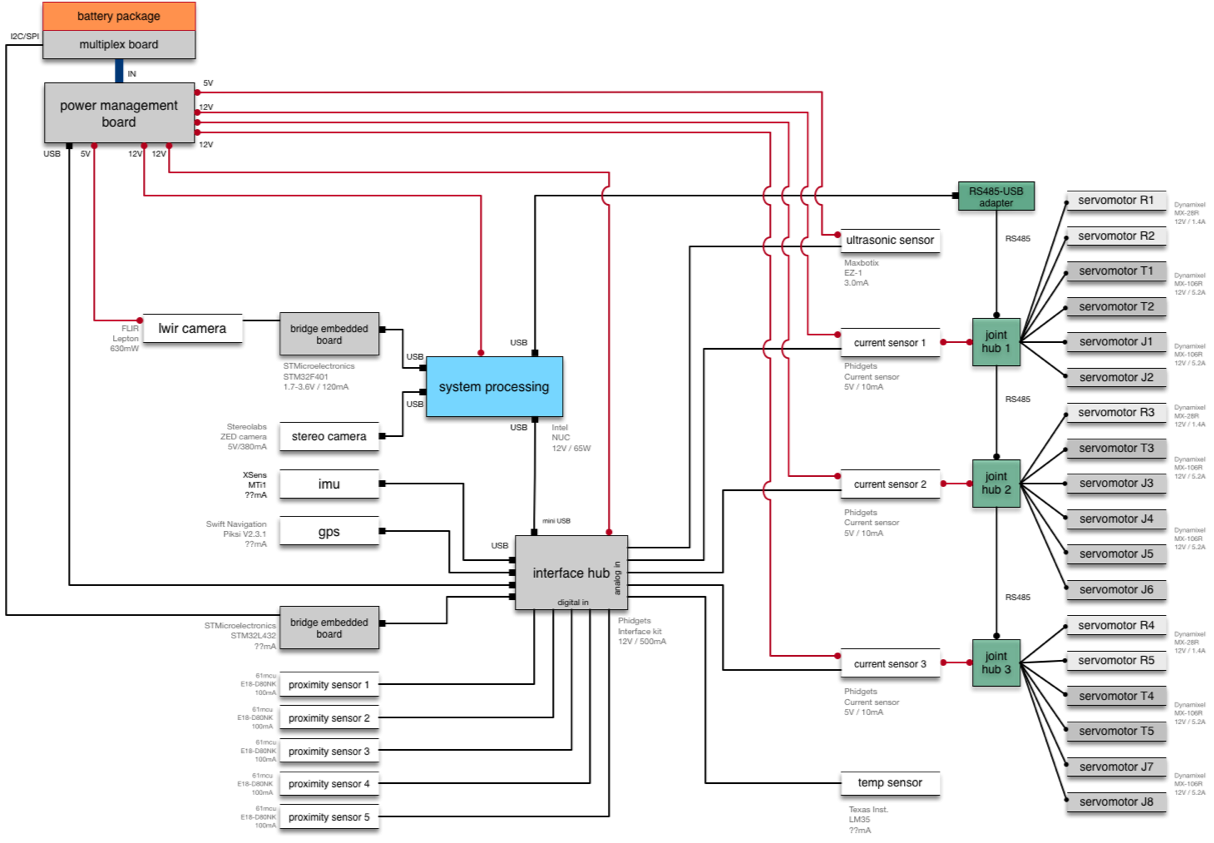
\includegraphics[width=1.0\textwidth]{./modeloesquematico2}
	%\fautor			 											 
\end{figure}													 
%----------------------------------------------------------

Como pode-se observar e de forma abrangente, os principais elementos que compõem o robô são:

\begin{itemize}
	\item 13 servomotores de 8.4Nm
	\item 05 servomotores de 2.5Nm
	\item 01 interface de IO
	\item 01 IMU
	\item 01 GPS
	\item 01 câmera stéreo
	\item 01 câmera LWIR
	\item 05 sensores de proximidade
	\item 01 sensor ultrassônico
	\item 01 sensor de temperatura
	\item 03 sensores de corrente
	\item 01 computador central para processamento das informações
	\item 01 placa de gerenciamento de energia
	\item 01 placa de gerenciamento de baterias
	\item 02 baterias de 14V
\end{itemize}

A Figura \ref{img:elirmodesq} é somente uma representação esquemática para o desenvolvimento da trabalho, no Apêndice \ref{Append:diagele} é apresentado os diagramas elétricos e eletrônicos para a compreensão total do sistema eletro-eletrônico considerado para este trabalho.


\subsection{Arquitetura geral do sistema robótico}
\label{ssec:arqg}
Para que o objetivo principal fosse atendido, a arquitetura do sistema foi elaborado compreendendo como um processo constituído de entradas e saídas, conforme representado pela Figura \ref{img:elirarq} . Logo, na arquitetura desenvolvida tem-se uma região sendo considerada como a região onde os sensores são os agentes coletores dos eventos desempenhado pelo robô; concomitantemente as saídas são consideradas como os atuadores que realizam a transposição e a translação do robô, nesta região faz parte também os displays de acesso as informações enviadas pelo robô, assim como a visualização da interface com o robô e o usuário.

%---------------picture------------------------------------
\begin{figure} [h!]	
	\caption{Arquitetura do robô ELIR.}
	\label{img:elirarq}											 
	\centering													 
	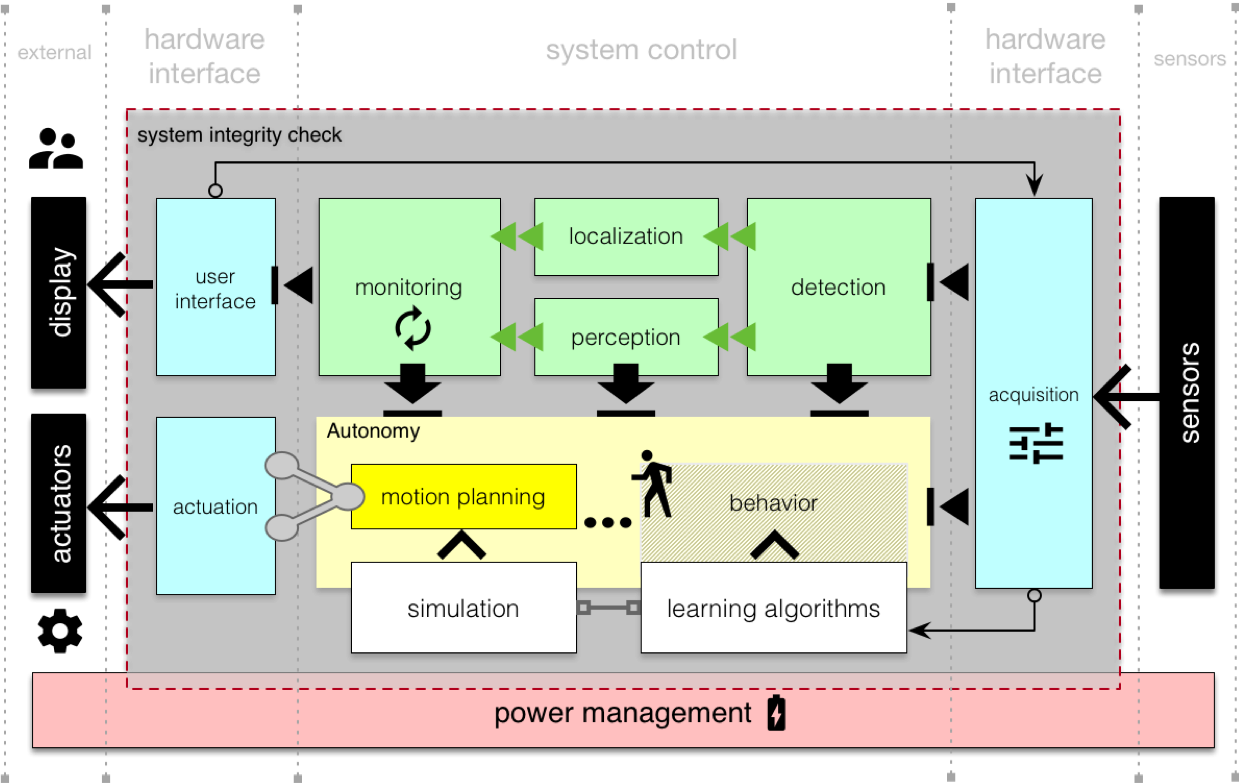
\includegraphics[width=1.0\textwidth]{./arquitetura2}
	%\fautor			 											 
\end{figure}													 
%----------------------------------------------------------

%continuar explicação


A estrutura da arquitetura apresentada se basea no \textit{framework} ROS, o qual possibilita a integração de todas as funcionalidades necessárias para o desenvolvimento do sistema robótico, trabalhando no conceito de nós, o \textit{framework} facilita a identificação de problemas durante a fase de desenvolvimento e também a modularização dos códigos.
\subsection{Arquitetura geral do sistema de Percepção}
\label{ssec:arqg}
A Percepção é o sistema de sensoriamento do robô e pode ser entendida como a forma que ele compreende o que esta ao seu redor. No projeto do robô ELIR, o sistema de percepção engloba a aquisição e a interpretação dos dados de todos os sensores envolvidos.

Na arquitetura geral deste sistema, mostrado na Fig. \ref{arqgeral}, estão representados as três camadas principais: \textit{Sensing}, \textit{Interface} e \textit{ROS Environment}.

\begin{figure}[!ht]
\centering
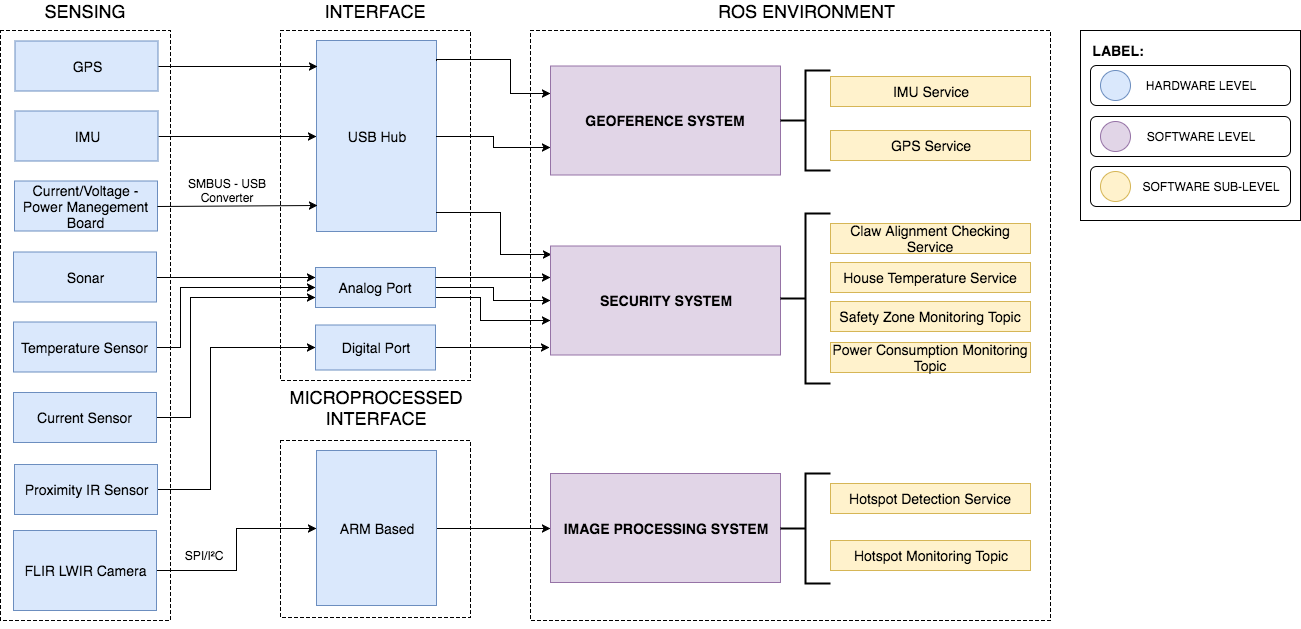
\includegraphics[width=15cm]{Figures/ArquiteturaPerceptionv2.png}
\caption{Arquitetura Geral da Perception}\label{arqgeral}
\end{figure}

 A etapa de \textit{Sensing} é composta por todos os processos de aquisição de dados de todos os sensores envolvidos no projeto. A camada de interface compreende a disponibilização destes dados para o ambiente de trabalho ROS. Essas duas etapas são camadas de \textit{hardware}. Por último, terá a camada de \textit{software}, a qual será feita no \textit{ROS Enviroment}, e que irá englobar todo o sistema de compreensão e interpretação dos dados provenientes do sistema de interfaceamento do robô.
 
 \pagebreak

\subsection{Arquitetura de software do sistema de Percepção}
\label{ssec:arqsp}


A arquitetura de software foi projetada em três camadas a fim de facilitar o desenvolvimento do sistema e simplificar o entendimento do mesmo. As camadas são:

\begin{itemize}
	\item \textit{User Interface Layer}
	\item \textit{Business Layer}
	\item \textit{Drvier Layer}
\end{itemize}
 
As camadas e seus componentes podem ser vistos na Fig.\ref{arqsoft}.

\begin{figure}[h]
	\centering
	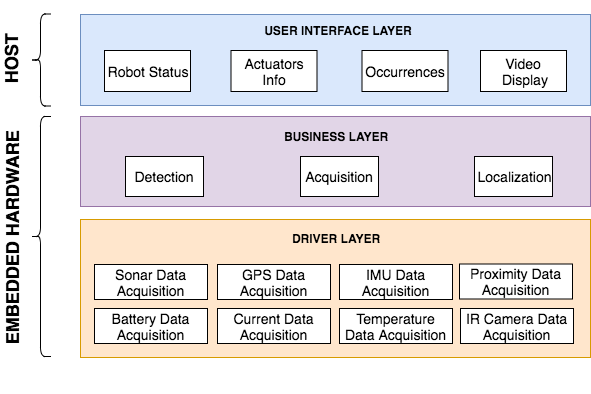
\includegraphics[width=15cm]{Figures/ArquiteturadeSoftware.png}
	\caption{Arquitetura Geral da Perception}
	\label{arqsoft}
\end{figure}

\subsubsection{Driver Layer}
	
A camada de \textit{Driver Layer} está diretamente relacionada a funcionalidade de aquisição de dados. Ela composta pelo \textit{hardware}, representado pelos sensores e seus respectivos drivers de comunicação. Desta forma, as subcamadas são nomeadas com o processo de aquisição de dados de cada sensor envolvido no projeto.

As subcamadas \textit{Current Data Acquisition}, \textit{Temperatura Data Acquisition}, \textit{Proximity Data Acquisition} e \textit{Sonar Data Acquisition} são responsáveis por adquirir as informações analógicas de seus sensores e transformá-los em dados da grandeza física a ser medida. Todas estas subcamadas utilizam a placa de interfaceamento Phidgets para o estabeler de comunicação entre o computador (NUC) e os sensores.

As subcamadas \textit{IMU Data Acquisition} e \textit{GPS Data Acquisition} são responsáveis pelo recebimento de dados da IMU e do GPS seguindo o protocolo de comunicação do fabricante. Esses dois módulos estão conectados ao \textit{hub} USB da placa de interfaceamento Phidgets. 

A subcamada de \textit{IR Camera Data Acquisition} é responsável pela aquisição de dados da câmera térmica, a qual se comunica via VoSPI (Video over SPI) com um microcontrolador de arquitetura ARM (STM32F401RE) e converte os dados para USB e os envia à NUC. 

Por último, a subcamada de \textit{Battery Data Acquisition} é responsável pelo estabelecimento da comunicação e coleta de informações com o \textit{Smart Charger} de bateria utilizando protocolo SMBus.

As conexões e diagramas elétricos podem ser vistos no apêndice \ref{Append:diagele}.

\subsubsection{Business Layer}

A camada \textit{business layer} é responsável por implementar a regra de negócio do sistema. As funcionalidades do sistema são representadas como sub-camadas da business layer, pois são elas responsáveis pelo processamento e coordenação dos dados adquiridos pela camada de aquisição.

\subsubsection{User Interface Layer}

A camada de \textit{User Interface} foi projetada para disponibilizar os dados para o operador. Nela será mostrado de forma resumida os dados mais relevantes do robô e da operação. Nesta camada existem três subcamadas: \textit{Robot Status Display, Actuators Display} e \textit{Video Display}. 

A subcamada \textit{Robot Status Display} disponibiliza os dados de integridade do robô como temperatura, corrente, tensão, nível de bateria, entre outras informações. A subcamada de \textit{Actuators Display} disponibiliza o dados de todos os motores do robô, como carga, temperatura, status e corrente. Por último, a subcamada de \textit{Video Display} mostra em tempo real o monitoramento realizado pela câmera térmica, possibilitando o usuário ver os componentes da linha que estão com temperatura elevada e até mesmo identificar pontos quentes.

A interface irá se resumir em duas telas: A tela principal com um layout de \textit{dashboard}, e outra que terá as informações dos atuadores. O \textit{dashboard} será um painel de monitoramento, no qual haverá as informações mais importantes da missão, como pode ser visto na apêndice \ref{fig:UI}. Essa tela irá mostrar as informações de integridade do robô, ocorrências e a imagem térmica. A tela dos atuadores irá mostrar de forma organizada, as informações já mencionadas, além da corrente total de cada \textit{hub} de motores. Pode-se observar a tela de atuadores na Figura \ref{fig:batt_protocol} no apêndice \ref{Append:wireframes}.


\section{Especificação técnica do sistema de Percepção}
\label{ssec:espt}

A construção do sistema de Percepção teve como base os requisitos técnicos do cliente. As especificações podem ser observadas abaixo:
\begin{itemize}
\item O sistema foi projetado para trabalhar com alimentação de 14V proveniente de baterias LiPo.
\item A máxima temperatura de trabalho na \textit{housing} é de 50 graus Celsius.
\item O sistema consegue detectar objetos através do sonar em uma faixa de servidão de 6.45 metros.
\item A obtenção de \textit{frames} da câmera IR acontece na taxa de 1 frame a cada dois segundos.
\item Em condições de sobretemperatura ou sobrecorrente o sistema alertará o operador.
\item O sistema não é protegido contra ingresso de água
\end{itemize} 


%--------- NEW SECTION ----------------------
\section{Desdobramento da função qualidade}
\label{sec:qfd}

O desenvolvimento do QFD\footnote{Quality Function Deployment, em português Desdobramento da Função Qualidade} foi desenvolvido na fase inicial do projeto, e é muito importante para compreender as relações entre os requisitos do cliente e os requisitos técnicos do projeto.

Neste primeiro ciclo do QFD os requisitos técnicos são avaliados e discutidos frente ao requisitos do cliente. Faz-se também necessário a avaliação das correlações entre os requisitos técnicos e avaliação destes requisitos com relação as possíveis soluções para o projeto, dessa forma de acordo com o Capítulo \ref{chap:intro} os competidores foram avaliados perante as metas estabelecidas para cada requisitos técnico e requisitos do cliente.
A Figura \ref{fig_qfd1} representa o primeiro ciclo do projeto.

%---------------------figure--------------------------------------------
\begin{figure}[htb]
	\begin{center}
		\includegraphics[scale=0.6]{Figures/elirqfd20180710cxf.png}
	\end{center}
	\caption{Desdobramento da Função Qualidade - primeiro ciclo.}
	%\legend{Fonte: \cite[p. 00]{asdkf}}
	\label{fig_qfd1}
\end{figure}
%-----------------------------------------------------------------------

Nesta avaliação de primeiro ciclo foi identificado alguns requisitos técnicos que devem ter uma maior preocupação no desenvolvimento do sistema, vale ressaltar que todos os requisitos devem ser buscados até alcançar as metas estabelecidas e apontadas no QFD (Figura \ref{fig_qfd1}).
Estes requisitos são os seguintes:
\begin{itemize}
	\item realizar as funções de forma autônoma	
	\item transpor obstáculos e cadeia de isoladores	
	\item realizar georeferenciamento	
	\item realizar odometria visual	
	\item deslocar-se através do  uso de energia elétrica (bateria VCC)	
	\item propulsão realizada por servomotores	
	\item realizar inspeção visual da linha, estrutura e obstáculos	
	\item realizar inspeção de temperatura da linha, estrutura e obstáculos	
	\item realizar inspeção da linha de servidão	
	\item disponibilizar os vídeos da missão	
	\item monitorar humidade e temperatura do protótipo	
\end{itemize}

%O QFD também aponta e avalia os concorrentes ao sistema idealizado neste projeto (conforme capítulo \ref{chap:estudo}) , tanto em relação aos requisitos apontados pelo cliente para aqueles técnicos.

Para o segundo ciclo do QFD, os requisitos técnicos foram confrontados com as funcionalidades pensadas para o sistema robótico, conforme Figura \ref{fig_qfd2}.

%---------------------figure--------------------------------------------
\begin{figure}[htb]
	\begin{center}
		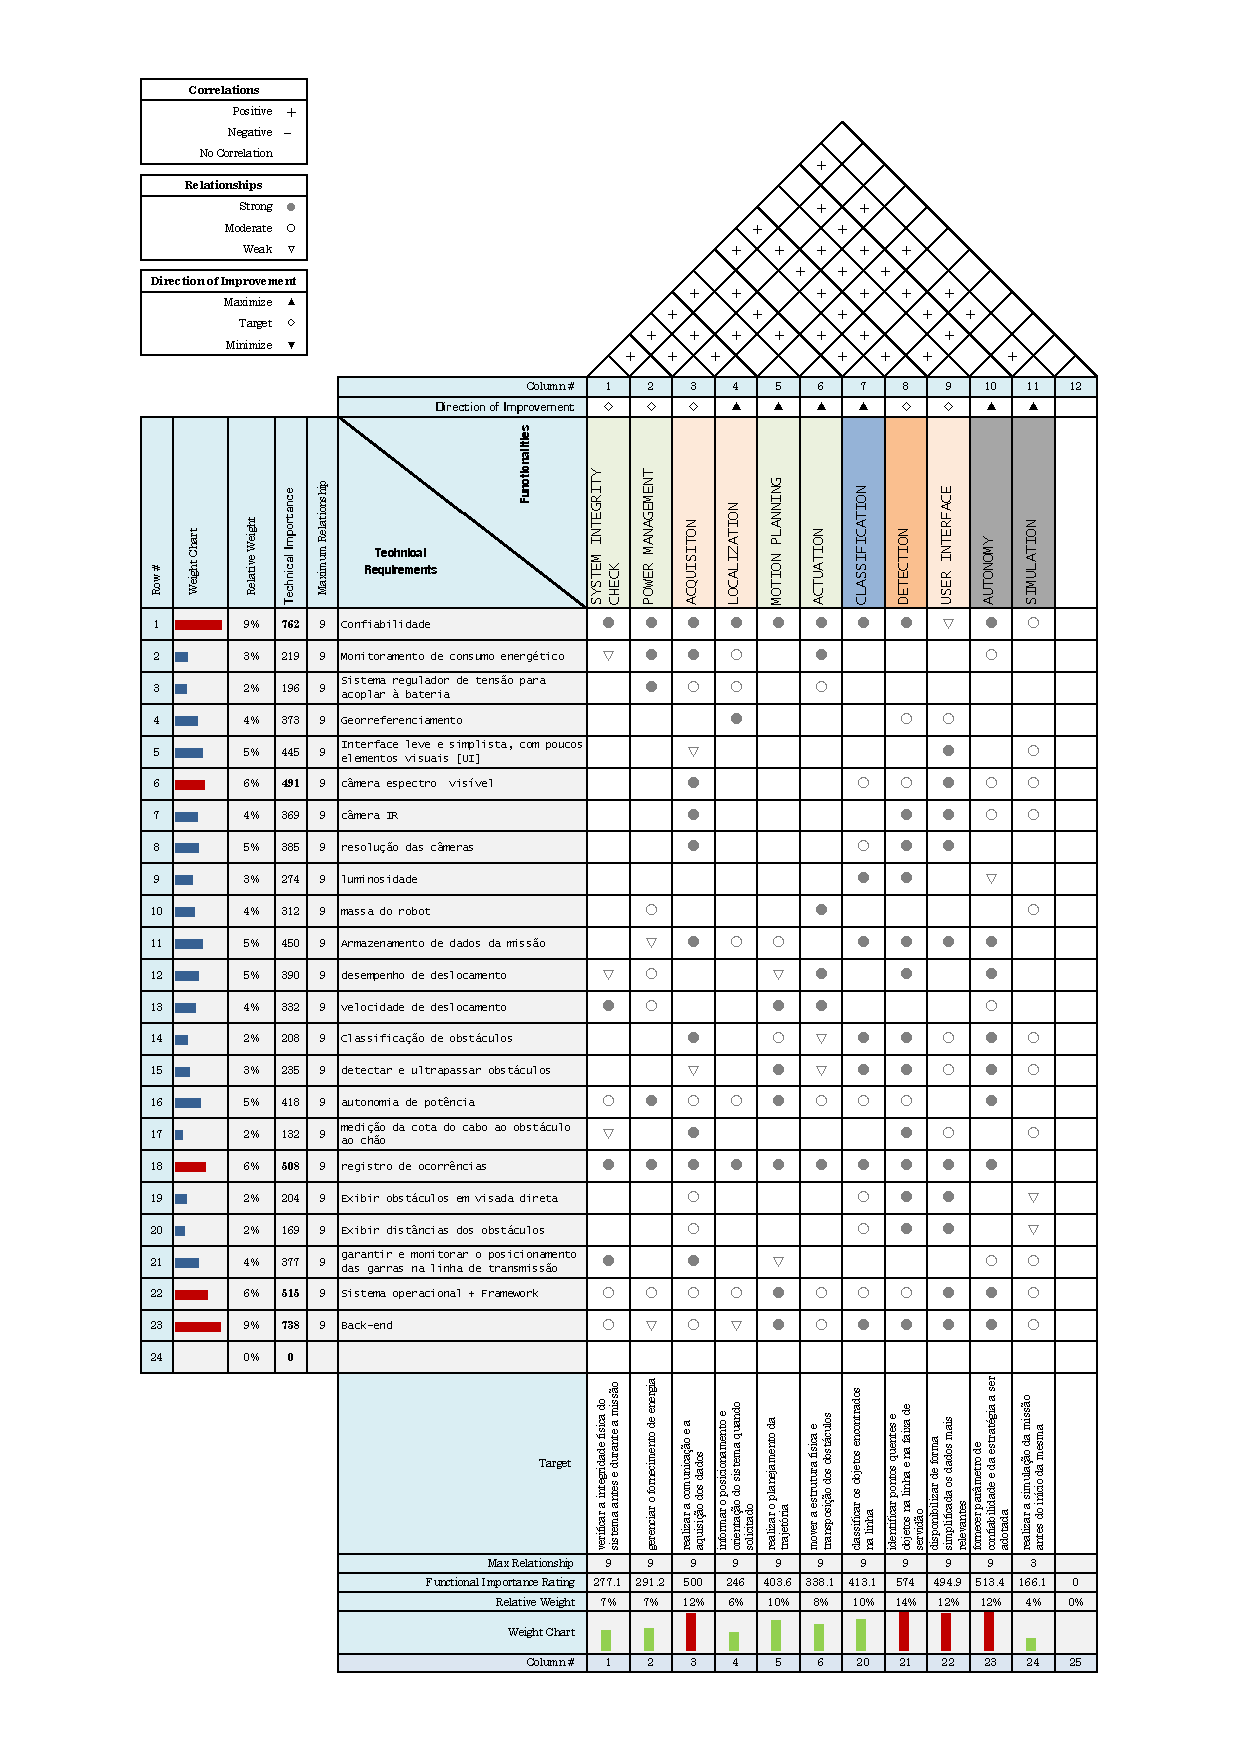
\includegraphics[scale=0.6]{Figures/elirqfd20180710txf.png}
	\end{center}
	\caption{Desdobramento da Função Qualidade - segundo ciclo.}
	%\legend{Fonte: \cite[p. 00]{asdkf}}
	\label{fig_qfd2}
\end{figure}
%-----------------------------------------------------------------------

Para mais detalhes quanto aos objetivos e as descrições das funcionalidades, as mesmas estão contidas na secção \ref{sec:espf}; encontra-se também no Apêndice \ref{Append:qfd}.

%\subsection{Requisitos técnicos}
%\label{ssec:reqt}
%asdfsadfdsf


    \chapter{Materiais e Métodos}
\label{chap:mat}
A criação de uma solução tecnológica vai além de um desenvolvimento e amadurecimento técnico-científico. O olhar sensível a problemática é o primeiro passo para a formação de um conceito. Problemas, desafios, dificuldades sempre existiram e sempre existirão mas a criação de uma solução para estes embates sempre vêm acompanhadas de uma primeira ideia motivadora, subjetiva e totalmente correlacionada às manifestações da natureza humana.

O processo de desenvolvimento de um sistema robótico não é diferente, existe uma motivação da equipe do projeto em cumprir o principal objetivo do conceito arquitetado abordado no Capítulo \ref{chap:intro}. Para garantir que esse objetivo seja alcançado são implementadas metodologias de desenvolvimento de projeto, que ajudam no acompanhamento e definição das atividades como meios para alcançar o fim que é a solução tecnológica.

No sistema de Percepção do robô ELIR a metodologia empregada consiste na divisão do projeto em três principais processos de construção de conhecimento, que são eles : a fase de conceitual e design, a fase de desenvolvimento e a fase de testes. O fluxograma com as fases do projeto está mostrado na Figura \ref{Fig:flux_proj}.

\begin{figure}[h]
	\centering
	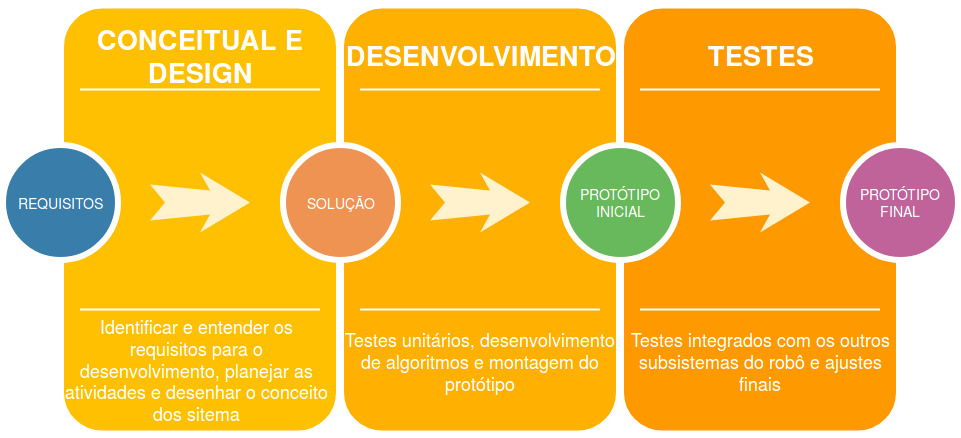
\includegraphics[width=16cm]{Figures/diagrama_proj.jpg}
	\caption{Fluxograma do Projeto}
	\label{Fig:flux_proj}
\end{figure}

O sucesso na execução de um projeto está fortemente relacionada com o seu gerenciamento, organização e planejamento. Por isso, conceitual e design é a fase mais importante do projeto pois ela representa o planejamento e previsão das demais fases. 

Nesta fase, há uma tempestade de ideias a serem organizadas de forma a chegarem em um conceito, um primeiro esboço do que se espera como solução final. Por isso, esta fase é marcada por uma série de reuniões entre a equipe de projeto, o orientador e o cliente a fim de coletar o máximo de informações de requisitos, premissas e necessidades que irão nortear o seu desenvolvimento. Apesar de ser considerada uma fase do projeto ela pode ser quebradas em duas etapas com papéis distintos. O conceitual busca a idealização enquanto o Design busca a avaliação da viabilidade técnica.

A fase de Desenvolvimento é o processo de construção da solução, a qual todas as ideias e planos da fase Conceitual e Design são colocadas em prática. O principal objetivo desta fase é fazer com que as funcionalidades do sistema deixem a área de idealização e se tornem práticas reais e mensuráveis. Por isso, o sucesso desta etapa é relacionado a expertise na fase de Conceitual e Design, nesta fase o planejamento do projeto deve ser fiel às necessidades reais do desenvolvimento.

A última fase do projeto é a fase de Testes. Nesta fase a solução tecnológica é validada por uma série de avaliações estatísticas que quantificam o projeto como todo, seja em desempenho, quanto em função tecnológica.  Esta é a fase de obtenção de resultados e por tanto representa a conclusão do projeto.


\section{Conceitual e Design}
Nesta etapa, são realizadas reuniões da equipe de projeto com o orientador técnico e cliente para definir os requisitos técnicos do projeto. Com base nos requisitos, a fase de Conceitual e Design busca elaborar: A arquitetura geral do sistema, especificação funcional, a arquitetura de software do sistema, os wireframes além da definição dos materiais a serem utilizados.

A arquitetura geral do sistema de Percepção do ELIR é um diagrama de blocos que mostra o fluxo de informações entre os subsistemas da percepção. Ela busca mostrar como as informações são obtidas, como são processadas e como são mostradas. 

A especificação funcional é uma descrição dos processos executados pelo sistema para cumprimento do objetivo geral. Por isso, cada funcionalidade é relacionada a um objetivo específico do projeto mostrado no capítulo 1. Para definição das funcionalidades é necessário descrever o seu objetivo, premissas, descrição, fluxograma de funcionamento e saídas. Esta é a etapa mais relevante da fase Conceitual e Design pois o desenvolvimento é norteado pelas funcionalidades do sistema. 

A arquitetura de Software é um esboço de como as funcionalidades são implementadas no campo de software. Por isso, são definidas as camadas de desenvolvimento e sua relação hierárquica. 

Por último, a definição dos materiais utilizados possui como base dois aspectos principais que são a disponibilidade dos materiais na instituição e a necessidade das funcionalidades do sistema. 

Após a construção do conceito do sistema, o projeto passa para uma segunda etapa que é a de desenvolvimento, esta etapa torna concreto e implementa as definições realizadas na etapa de  Conceitual e Design, esta nova etapa está explicada em detalhes na seção a seguir.

\section{Desenvolvimento}

 Nesta etapa são realizados os testes unitários dos sensores do sistema, o projeto  e fabricação de peças mecânicas para suportar os sensores, são implementados os drivers dos sensores e protocolos de comunicação além da implementação das funcionalidades do sistema e da interface gráfica. 

Os teste unitários dos  sensores do projeto servem para validar o funcionamento e avaliar se suas especificações atendem os requisitos impostos pelo cliente. No teste são coletadas amostras dos dados recebidos de cada sensor e esses dados são avaliados a partir de uma distribuição normal. A distribuição normal assim como qualquer distribuição estatística serve para determinar a probabilidade de ocorrência do fenômeno relacionado aos dados. Logo, é usada no ELIR para avaliação de desempenho dos sensores.

O projeto mecânico do ELIR foi fornecido pelo próprio cliente do projeto. Desta forma, o desenvolvimento de partes mecânicas do sistema de percepção se limitou ao projeto de suportes para a integração dos sensores na parte física do robô. Para realizar estes projetos, foi estudado os desenhos mecânicos de cada sensor a fim de projetar peças menos invasivas.

A principal função de um sistema de Percepção é a coleta e tratamento dos dados de seus sensores. Para que estes dados sejam reunidos é necessário que no fim todos os sensores se comuniquem de maneira semelhante, ou seja, utilizando o mesmo protocolo de comunicação. A ferramenta utilizada para a integração destes dados é um framework de robótica. O framework serve para reunir dados de diferentes fontes em um mesmo ambiente, com o mesmo padrão de formatação. Por isso, o desenvolvimento de drivers para cada sensor é extremamente importante pois ele garante a conversão do protocolo de comunicação intrínseco do sensor para o padrão utilizado no framework de robótica.


\section{Testes}
Como descrito anteriormente a fase de testes reflete um processo de coleta de dados e utilização de métodos estatísticos para chegar na probabilidade de ocorrência dos fenômenos.  

Os testes integrados do sistema de Percepção possuem como objetivo a comprovação das funcionalidades do projeto e foram divididos em dois testes principais.

O primeiro teste busca a comprovação do sistema de Detecção, neste teste é confirmado se na ocorrência de um ponto quente ou identificação de objetos fora da faixa de servidão geram uma mensagem de alerta no arquivo de log do robô.

O segundo teste busca analisar se a interface gráfica mostra em tempo real todas as informações relevantes para o robô. O sucesso deste teste comprova o funcionamento do sistema de Percepção e por isso é considerado o mais relevante para o projeto.
 
    \chapter{Resultados}
\label{chap:result}

As funcionalidades do sistema de percepção foram validadas a partir de duas etapas de testes. Os testes unitários buscam a validação do funcionamento individual dos sensores, enquanto os testes integrados validam o funcionamento dos sistemas e funcionalidades, ou seja, todos os componentes em conjunto. A descrição dos testes realizados e dos resultados obtidos por eles está descrita abaixo.

Para mais detalhes sobre as conexões eletro-eletrônicas, pode-se ver o apêndice \ref{Append:diagele}.

%--------- NEW SECTION ----------------------
\section{Testes unitários}
\label{sec:testu}

	\subsection{Câmera Térmica}
	
		A câmera térmica Lepton, do fabricante FLIR, se comunica por VOSPI. Logo, foi necessário utilizar um driver para converter os dados da câmera e disponibiliza-los para a USB. Uma placa de desenvolvimento Nucleo STM32F401RE com o driver disponibilizado por \citeonline{groupgets} foi utilizada para essa situação.
		
		\begin{figure}[!ht]
		   \centering
		   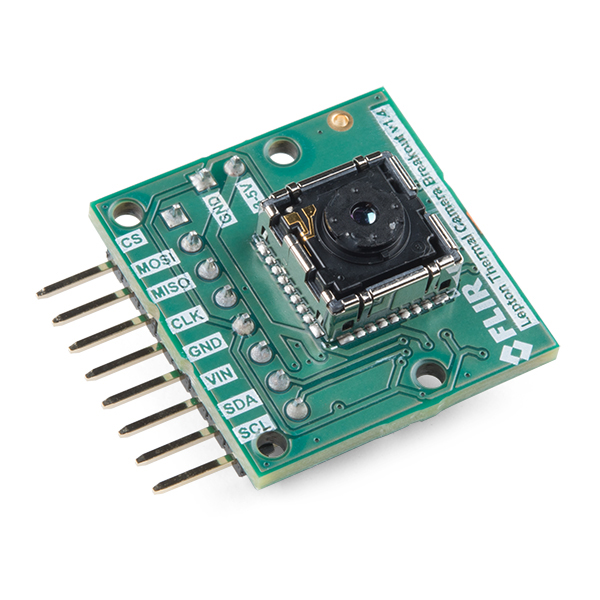
\includegraphics[width=6cm]{Figures/lepton_flir.jpg}
		   \caption{Lepton LWIR}
		   \label{fig:lepton}
		\end{figure}
		
		O driver coleta os frames e verifica se o mesmo foi adquirido corretamente, após isso, envia para a USB seguindo o padrão de mensagem mostrado na Figura \ref{fig:framemsg}.
		    
		\begin{figure}[!ht]
		   \centering
		   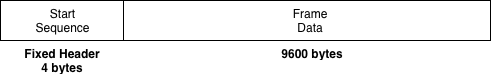
\includegraphics[width=14cm]{Figures/frame_msg.png}
		   \caption{Mensagem do frame da câmera}
		   \label{fig:framemsg}
		\end{figure}
	
	    No início de cada mensagem, há uma sequência de quatro \textit{bytes} para confirmar a transferência dos dados. Após a confirmação por um \textit{script} em python, inicia-se o processo de aquisição do \textit{frame}. Cada \textit{frame} é composto por 4800 \textit{pixeis}, sendo 80 na horizontal e 60 na vertical. Além disso, cada \textit{pixel} possui 2 \textit{bytes} de profundidade de cor, correspondendo a 9600 \textit{bytes} de informação para cada \textit{frame}. Na Figura \ref{fig:frame_esque}, pode-se observar uma representação do \textit{frame} da câmera.
	    
	%\pagebreak
	
		\begin{figure}[!ht]
		   \centering
		   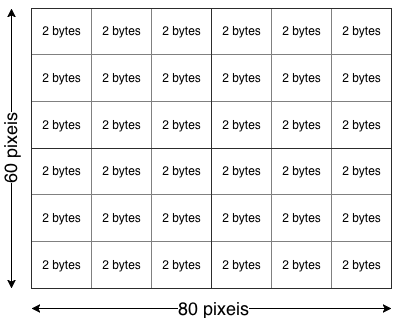
\includegraphics[width=10cm]{Figures/frame_esque.png}
		   \caption{Esquemático do \textit{Frame} da Câmera Térmica}
		   \label{fig:frame_esque}
		\end{figure}
		
		No \textit{script} de aquisição de \textit{frames}, cada \textit{pixel}, foi convertido para uma escala de cinza de 8-bits (1 \textit{byte}). Conversão necessária para trabalhar com a biblioteca de processamento de imagens OpenCV.
		    
		A OpenCV (Open Source Computer Vision Library) é uma biblioteca gratuita para operações de imagens tanto para uso acadêmico e para uso comercial, contendo interface para C++, Java e Python. A mesma foi desenvolvida com foco em eficiência computacional para sistemas de tempo real.

		O processamento da imagem térmica pode ser dividido em três etapas:  pré-processamento, realce e busca de contornos.
		
		\begin{itemize}
			\item Pré-processamento: refere-se ao processamento inicial de dados brutos para remoção de ruído e redimensionamento.
			\item Realce: visa melhorar a qualidade da imagem, permitindo uma melhor discriminação dos objetos presentes na mesma.
			\item Na busca de contorno é utilizado algoritmos para buscar objetos brancos.
		\end{itemize}
		
		\subsubsection{Pré-processamento}
		
		Primeiramente, a imagem da câmera de 80x60 pixeis é escalonada para uma imagem de 400x300 pixeis, com objetivo de inseri-la, no final do processamento de imagem, na interface gráfica. Para isso, é utilizado uma interpolação bicúbica, utilizando quatro pixeis vizinhos para a operação.
		
		As imagens capturadas por câmeras digitais nem sempre representam fielmente a realidade. Os sinais analógicos possuem ruídos, que são sinais interferentes de natureza aleatória que provoca a degradação do sinal de interesse durante seu processamento \cite{fabris}.
		
		Em sistemas de captura de imagem, existem três categorias principais de ruído, que são os aleatórios, os sistemáticos e os chamados de \textit{banding noise}. Os aleatórios são usualmente causados quando se utiliza o sensor com baixa exposição, ou seja, uma velocidade de captura muito alta, causando uma flutuação das cores sobre a atual intensidade da imagem. Os ruídos sistemáticos são causados geralmente por uma longa exposição do sensor a luz e por altas temperaturas. O \textit{banding noise} é introduzido no momento em que o sensor está convertendo os dados analógicos para digital, e está diretamente relacionado ao tipo de tecnologia aplicada no mesmo (CCD ou CMOS). Na imagem abaixo, pode-se observar os três tipos de ruídos.
	
		\begin{figure}[!ht]
		   \centering
		   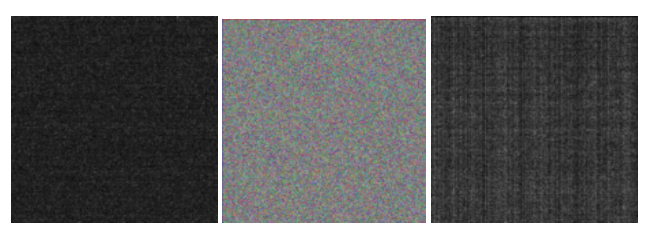
\includegraphics[width=14cm]{Figures/noise.png}
		   \caption{Exemplo de um ruídos em imagens. Aleatório, sistemático e banding, da esquerda para a direita.}
		   \label{fig:noise}
		\end{figure}
		
		Antes de entrar na etapa de realce, é necessário atenuar esses ruídos da imagem, caso contrário, os mesmos também serão amplificados no procedimentos posteriores. Como se sabe que o fundo da imagem das digitais são uniformes, qualquer componente de alta frequência deve ser removida. Para isso, foi utilizado um filtro passa-baixa comumente chamado de \textit{blur}. Na figura \ref{fig:img_80graus}, pode-se observar a imagem original.
			
		\begin{figure}[!ht]
		   \centering
		   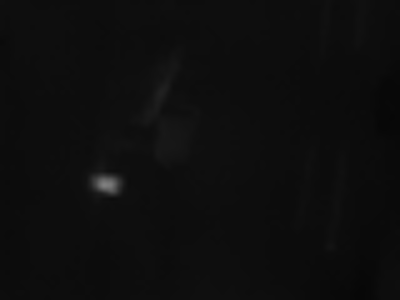
\includegraphics[width=8cm]{Figures/flirphoto.png}
		   \caption{Imagem Original}
		   \label{fig:img_80graus}
		\end{figure}
		
		Basicamente, o filtro realiza uma convolução entre um operador e a imagem de interesse tirando uma média dos pixeis vizinhos. O operador é mostrado na Equação \ref{equ:kernel}.
		
		\begin{equation}
			K = \frac{1}{25}\cdot \begin{bmatrix}
			 1  1  1  1  1\\ 
			 1  1  1  1  1\\ 
			 1  1  1  1  1\\ 
			 1  1  1  1  1\\ 
			 1  1  1  1  1 
			\end{bmatrix}
			\label{equ:kernel}
		\end{equation}
		
		Essa matriz é fixada em cima de um pixel, e é somado o valor de todos os pixeis dentro do operador. Após isso, é tirado uma média dos valores, substituindo o valor do pixel central por ela. No caso da Equação \ref{equ:kernel}, é uma matriz unitária 5x5 multiplicada por uma constante igual ao inverso do quadrado da dimensão da mesma. A frequência de rejeição pode ser alterada ao aumentar ou diminuir a dimensão da matriz. Na Figura \ref{}, pode-se observar o efeito do filtro.
		
		\begin{figure}[!ht]
		   \centering
		   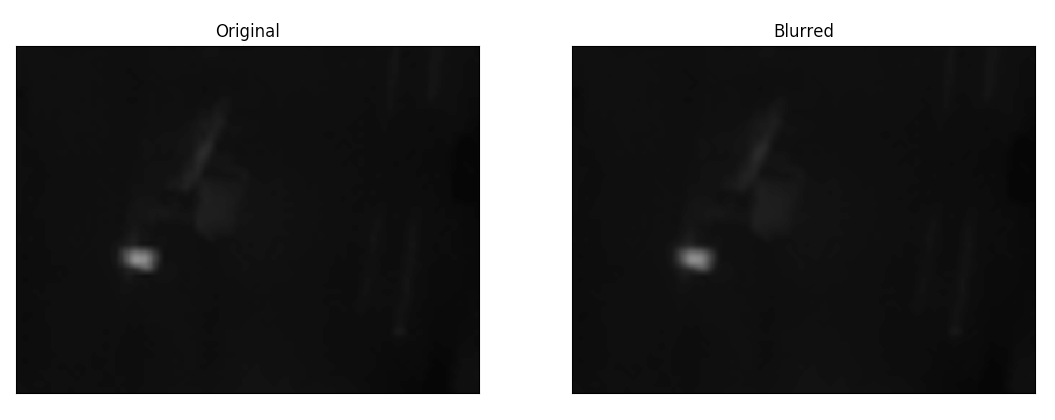
\includegraphics[width=16cm]{Figures/blur.png}
		   \caption{Imagem Original e após o filtro \textit{blur}}
		   \label{fig:blur}
		\end{figure}
		
		Após o pré-processamento, pode-se dar inicio ao procedimento de realce dos dados relevantes da imagem.
	
	\subsection{Sonar EZ-1}
		O sonar EZ-1 da MaxBotix possui saída analógica referente a distância medida. Para testa-lo, foi utilizada uma das entradas analógicas da Phidgets.
		
		\pagebreak
		
		\begin{figure}[!ht]
		   \centering
		   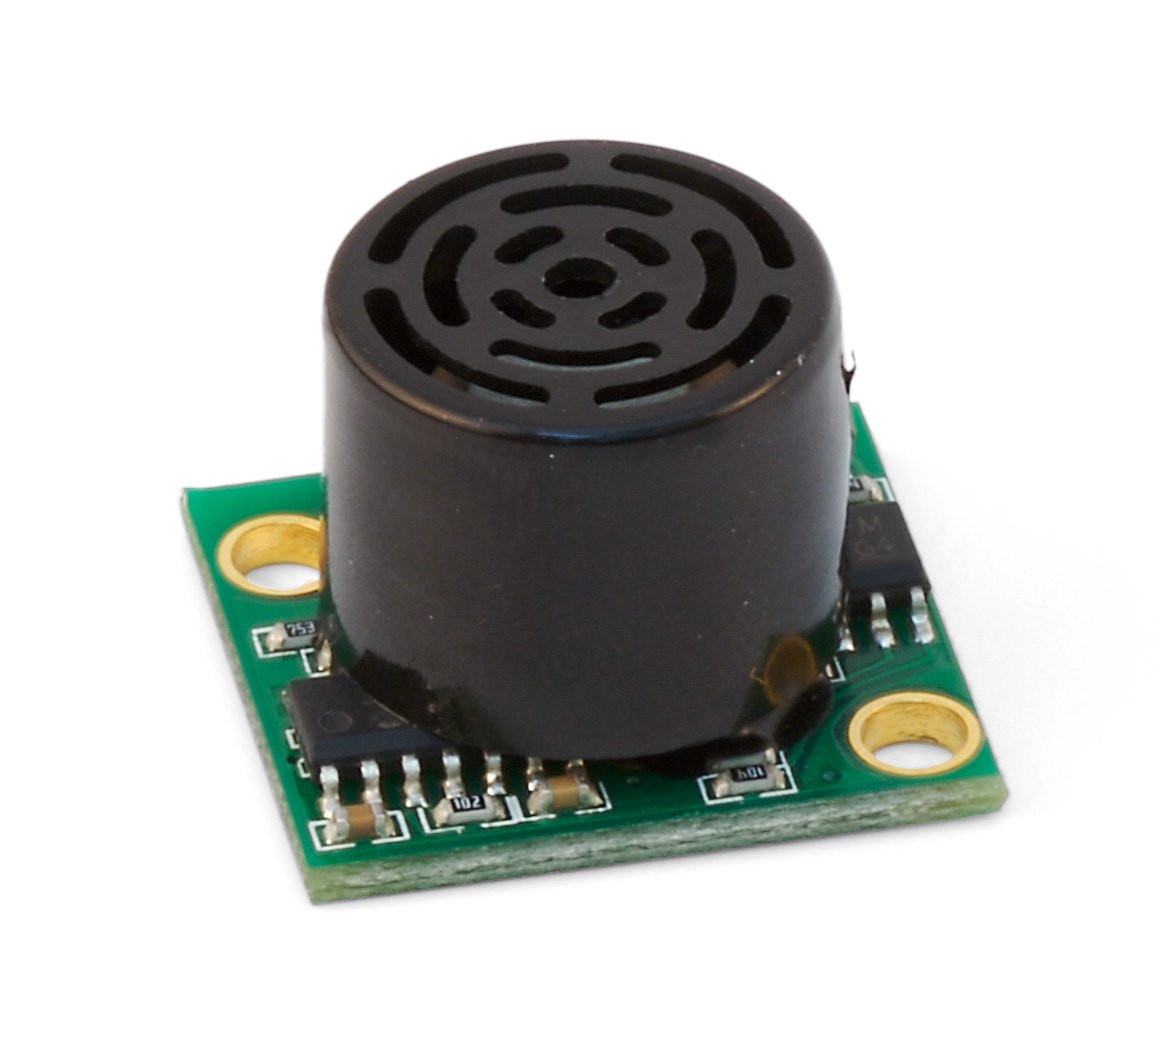
\includegraphics[width=8cm]{Figures/ez1.jpg}
		   \caption{Sonar EZ-1}
		   \label{fig:ez1}
		\end{figure}
		
		A comunicação da Phidgets com com a NUC é feita via USB, contudo, é necessário a instalação dos drivers obrigatórios da placa no linux. Além disso, é necessário a instalação do módulo python respectivo da placa, dessa forma, permitindo a utilização de classes e métodos para controle da comunicação com os sensores.
		
		Com os respectivos drivers e módulos da phidgets instalados no computador, foi necessário apenas conectar os terminais alimentação e saída analógica do sensor nos conectores correspondentes da Phidgets e executar um \textit{script} de leitura da tensão nas entradas analógicas fornecido pela própria fabricante. 
		
		Ao executar o código, recebe-se, no intervalo de dez segundos, todas as leituras de tensão efetuadas no sensor. Notamos que ao afastar o obstáculo do sonar o valor de tensão aumentava e quando aproximavamos o obstáculo o valor de tensão diminuía. Após feita a conversão de tensão para unidades métricas através das informações disponibilizadas no \textit{datasheet}, foi possível validar o sensor.
	
	\subsection{Sensor de Proximidade}
		O sensor de proximidade E18-D80NK funciona de maneira bastante simples. O módulo possui um emissor e um receptor de feixes infra-vermelhos, o qual identifica se há ou não um objeto próximo devido a reflexão, liberando assim, um sinal de nível alto caso positivo e nível baixo caso negativo.
		
		\begin{figure}[!ht]
		   \centering
		   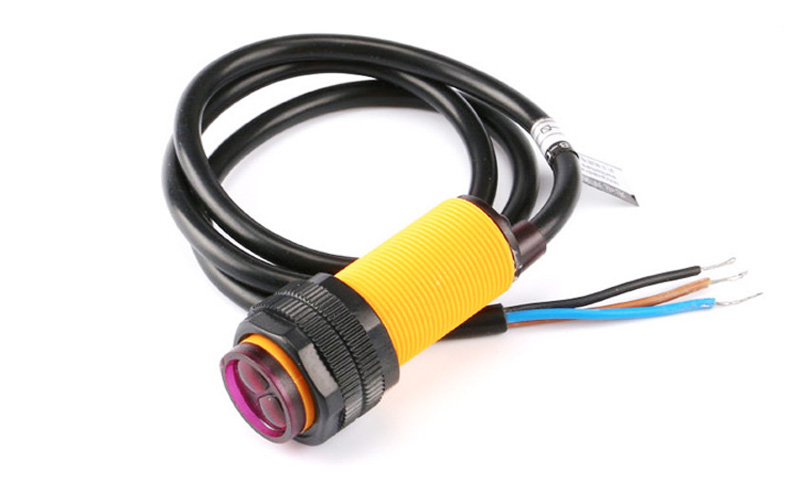
\includegraphics[width=8cm]{Figures/proximity_sensor.jpg}
		   \caption{Sensor de proximidade E18-D80NK}
		   \label{fig:E18-D80NK}
		\end{figure}
		
		Por questão de sinalização, o fabricante adicionou um LED, que ao identificar algum objeto próximo, acende-se. Com isso, logo após alimentar o sensor já era possível ver o seu funcionamento. Entretanto, ainda era necessário verificar se a saída digital referente a detecção estava em devido funcionamento.
		
		Para isso, foi utilizada a placa de interfaceamento Phidgets assim como no tópico anterior. O que diferiu nesse teste para o anterior é que o sensor foi acoplado em uma entrada digital, em vez de uma analógica, assim como o \textit{script} executado foi para comunicação com as entradas digitais. O código, também disponibilizado pela fabricante, notifica a mudança de estado da saída dos sensor, dessa maneira podendo ser validada.
		
	\subsection{\textit{Smart Charger}}
    
	    A placa de gerenciamento e carregamento das baterias DS325A, da empresa Inspired Energy, funciona a partir do protocolo de comunicação SMBus. Informações das baterias como temperatura, corrente, carga, entre outras podem ser solicitadas através do seguinte protocolo de leitura.
	    
	    \begin{figure}[!ht]
			   \centering
			   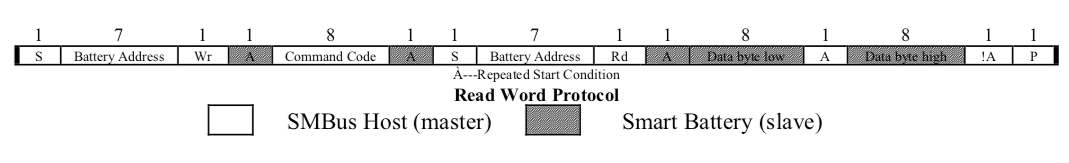
\includegraphics[width=16cm]{Figures/batt_protocol.png}
			   \caption{Protocolo de comunicação do \textit{Smart Charger} e das baterias}
			   \label{fig:batt_protocol}
		\end{figure}   
		
		No qual é necessário enviar primeiro o endereço de 7 bits da bateria de interesse, seguido do comando referente a que informação está se requisitando. Após isso, inicia-se o processo de leitura das informações da bateria.
		
		O driver de comunicação foi desenvolvido em uma placa de desenvolvimento Nucleo STM3L432KC para disponibiliza-los na USB do computador. Além disso, um \textit{script} em python foi escrito para requisitar essas informações do microcontrolador.
	    
	    Os dados foram convertidos para suas respectivas grandezas, dessa maneira, foi possível validar as informações obtidas.
    
    \subsection{Sensor de Temperatura}
    
	    O sensor de temperatura LM35 possui uma saída analógica e com comportamento linear entre a tensão de saída e a temperatura medida.
	    
	    \begin{figure}[!ht]
			   \centering
			   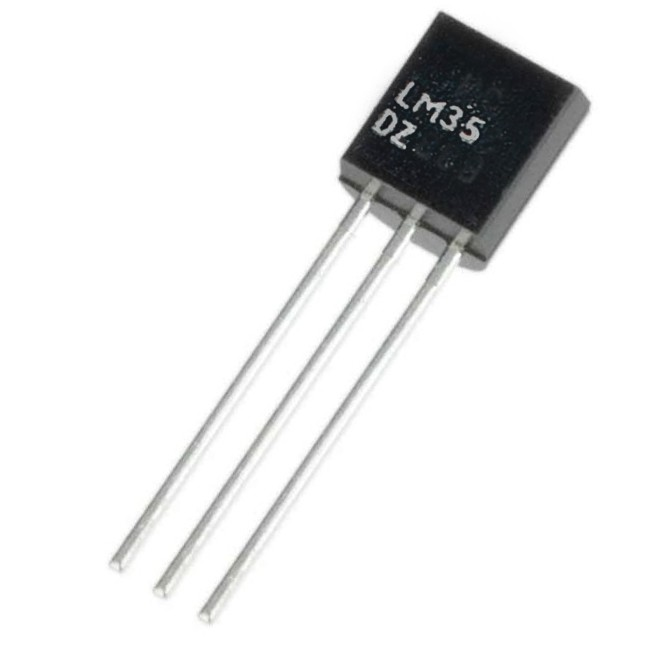
\includegraphics[width=6cm]{Figures/lm35.jpg}
			   \caption{Sensor de Temperatura LM35}
			   \label{fig:LM35}
		\end{figure}
	   
	    O componente foi testado em uma das entradas analógicas da Phidgets, e utilizando o mesmo algoritmo de leitura de tensão já mencionado para realizar a obtenção de dados. Para verificar a resposta do sensor, foi medido o valor de tensão de saída para uma sala com ar-condicionado e para um ambiente externo com auxílio de um termômetro de referência.
	    
	    Os valores de tensão foram convertidos para graus Celsius, através da correlação disponível no \textit{datasheet}, validando assim o sensor.
    
    \subsection{GPS}
    
	    O GPS Piksi v2.3.1, da Swift Navigation, possui um console disponibilizado pelo próprio fabricante, porém como se tinha em mãos uma versão antiga do aparelho, foi necessário descobrir qual a versão compatível do \textit{software}.
	    
	    \begin{figure}[!ht]
				   \centering
				   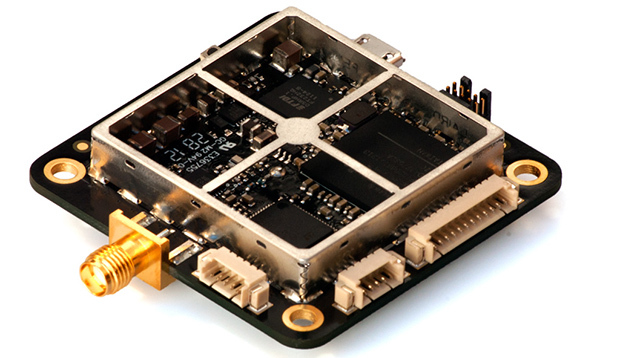
\includegraphics[width=6cm]{Figures/gps.jpg}
				   \caption{GPS Piksi v2.3.1}
				   \label{fig:GPS}
		\end{figure}
			    
	     O console foi instalado, o GPS foi conectado na USB do computador e a antena devidamente acoplada. Essa versão em específico precisa de quatro satélites para realizar os cálculos de coordenadas, e em ambientes fechados, a recepção de sinal é bastante degradada. Para contornar essa situação, o dispositivo foi iniciado em modo de simulação em seu console, mostrando assim, os dados de longitude e latitude.
	     
	     Posteriormente, a antena foi levada a um ambiente externo e verificou o funcionamento do GPS fora do modo de simulação.    

	\subsection{IMU}
	    
	    A IMU Mti-1, fabricado pela Xsens, possui um console que é disponibilizado no próprio pendrive de instalação que vem junto ao sensor.
	    
	    \begin{figure}[!ht]
		   \centering
		   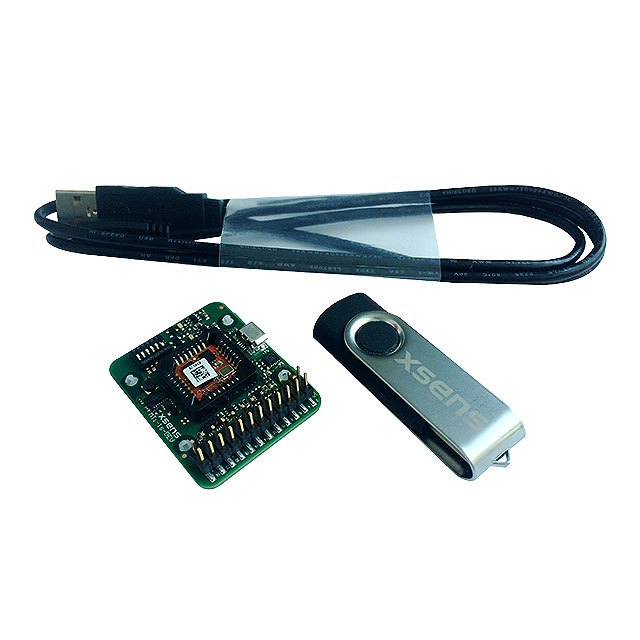
\includegraphics[width=8cm]{Figures/imu.jpg}
		   \caption{IMU Xsens Mti-1}
		   \label{fig:IMU}
		\end{figure}
	    
	     Com o console instalado, foi apenas necessário conectar a IMU a uma das portas USB do computador. Na própria interface gráfica já aparece as informações de orientação do dispositivo, informando a orientação nos três eixos de referência e velocidade angular.
	
%--------- NEW SECTION ----------------------
\section{Integração no ROS}
\label{sec:rosinte}

	Após os testes unitários de cada sensor, deu-se inicio à integração dos sensores no ambiente ROS para construção do sistema de Percepção. A descrição da metodologia empregada para embarcar cada um dos sensores no framework de robótica está mostrada nos tópicos abaixo.

\subsection{Phidgets}
     Após a fase de testes unitários, foi necessário desenvolver o \textit{package} de comunicação da phidgets no ROS. Esse \textit{package} é responsável pela aquisição dos dados de todos os sensores analógicos e digitais conectados a Phidgets.
     
     Os nós foram desenvolvidos utilizando como base o módulo \textit{python} da Phidgets. Ele consiste em uma classe e cada objeto desta, representa um componente conectado a placa de interface. Ao declarar o objeto, se faz necessário informar o canal, o nome do dispositivo, o tipo de porta (digital ou analógico) e o nome do tópico a ser disponibilizado os dados. 
     
     No construtor da classe os dados referentes aos dispositivos são coletados e um \textit{publisher} do ROS é inicializado. Este  \textit{publisher} faz com que periodicamente os dados de tensão(canais analógicos) ou status da porta(canais digitais) sejam coletados e disponibilizados no tópico escolhido pelo usuário. 
     
     No script original foram criados seis objetos da classe no \textit{main loop}, correspondentes aos cinco sensores de proximidade conectados a portas digitais e ao sonar conectado na porta analógica.
     
\subsection{Smart Charger}
     
     O script utilizado no teste unitário para receber os dados provenientes do \textit{smart charger} no computador foi utilizado como base para a construção do nó no ambiente ROS.
     
     O nó funciona enviando um \textit{byte} pré-definido para dar início ao processo de transmissão de dados da bateria. A recepção do \textit{byte} pela Nucleo L432KC inicia a leitura dos dados da bateria, como mostrado no tópico anterior. Logo após isso, ocorre o envio das informações em sequência para o computador, como pode ser visto abaixo:
      
      \begin{figure}[!ht]
		   \centering
		   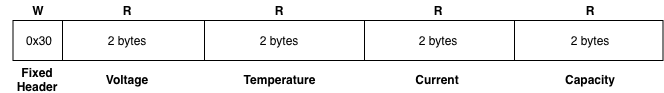
\includegraphics[width=16cm]{Figures/batt_protocol_2.png}
		   \caption{Mensagem entre a Nucleo L432KC e o nó referente às baterias}
		   \label{fig:battprotocol2}
		\end{figure}
		      
      No nó do ROS essas informações são recebidas via serial e convertidas para sua devidas unidades segundo o \textit{datasheet} do fabricante. Esses dados são colocados em um formato de mensagem chamado de Battery e publicadas em um tópico do ROS. O nó criado para a \textit{smart charger} está mostrado no anexo XX.
     
     \subsection{Câmera Térmica}
     
     A integração da câmera no ROS foi feita em duas etapas, que na prática foram representadas como dois nós:
     
     \begin{itemize}
         \item O primeiro com objetivo da aquisição dos dados da câmera e sua disponibilização em um tópico.
         \item O segundo nó é responsável por todo o tratamento da imagem e detecção dos pontos quentes.
     \end{itemize}
     
     Para a aquisição dos dados, no primeiro nó, foi utilizado basicamente o mesmo algoritmo que no teste unitário, porém com a integração das bibliotecas do ROS para publicar os \textit{frames} em forma de \textit{Numpy arrays} em seus devido tópico.
     
     No segundo nó foi utilizado a biblioteca OpenCV para realizar o processamento da imagem. Primeiramente, o frame disponibilizado pelo nó de aquisição é adquirido subscrevendo do seu respectivo tópico. Para retirar o aspecto "pixelado" da imagem da câmera, devido a sua baixa resolução (80x60 pixeis), foi necessário realizar uma interpolação cúbica para redimensionar a imagem para uma resolução de (400x300 pixeis), obtendo assim uma imagem mais detalhada. 
     
     Com a imagem já redimensionada, é aplicado um filtro \textit{blur} para eliminar altas frequências que podem interferir na binarização (\textit{thresholding}) que será feita na imagem.
     
     Após o filtro, o frame é binarizado com o objetivo de facilitar a identificação dos pontos quentes através de um algoritmo de busca de contornos.
     
     O esquemático abaixo mostra simplificadamente o processo de tratamento da imagem.
     
    \begin{figure}[!ht]
    	\centering
    	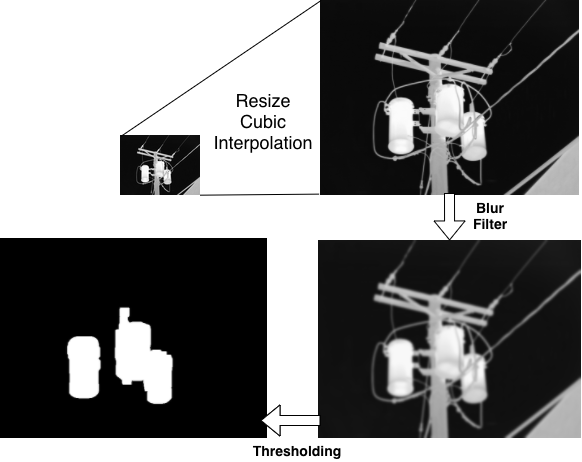
\includegraphics[width=14cm]{Figures/image_proc.png}
    	\caption{Esquemático do processamento da imagem} \label{imgproc}
	\end{figure}
     
     \subsection{GPS}
     
     Para o GPS, foi utilizado um driver disponibilizado no GitHub por \citeonline{ethz} com licensa livre para embarcar o dispositivo no ROS.
     
     O \textit{package} possui nós que publicam em tópicos as informações de coordenadas obtidas do GPS.
     
     \subsection{IMU}
    Foi utilizado o driver da IMU disponibilizada pela própria fabricante Xsens para embarcar a IMU no ROS. O driver de licença livre é disponibilizado no GitHub da própria empresa.
%--------- NEW SECTION ----------------------
\section{Testes integrados}
\label{sec:testi}
asdfadsfsdfs

%--------- NEW SECTION ----------------------
%\section{Avaliação da prontidão tecnológica}
%\label{sec:trl}
%
%Uma das ferramentas conhecidas para a avaliação de tecnologias é a matriz TRL desenvolvida pela NASA\footnote{National Aeronautics and Space Administration} e que permitir definir o nível de maturidade de uma tecnologia. Entende-se que a tecnologia é definida como a aplicação prática do conhecimento para criar a capacidade de fazer algo inteiramente novo de forma inteiramente nova, o que difere da pesquisa científica que engloba a descoberta de um novo conhecimento da qual a tecnologia é derivada.
%
%A importância do uso dessa avaliação, encontra seu respaldo no quesito de nortear o desenvolvimento do projeto na minimização dos gastos oriundos de uma orçamentação e também no conhecimento das tecnologias plausíveis para o desenvolvimento da solução requerida.
%
%%\section{A matriz BTRL}
%Todo projeto foi acompanhado por uma cadência de avaliações ao longo das fases do projeto. Estas avaliações seguem as diretrizes da ISO 16290, a qual estabelece níveis do quanto uma tecnologia está desenvolvida, tomando como base este procedimento e levando em consideração as avaliações de risco para um projeto de R\&D\footnote{Research and Development}, criou-se o BTRL\footnote{BIR Technology Readiness Level}. 
%
%% Please add the following required packages to your document preamble:
%% \usepackage[table,xcdraw]{xcolor}
%% If you use beamer only pass "xcolor=table" option, i.e. \documentclass[xcolor=table]{beamer}
%%\begin{sidewaystable*}
%\begin{table}[h]
%\centering
%\caption{Matriz do Nível de Prontidão Tecnológia do Senai Cimatec.}
%\begin{adjustbox}{width=1\textwidth}
%\label{tabela:BTRL}
%\begin{tabular}{lc|p{1.5cm} p{1.5cm} p{1.5cm} p{1.5cm}}
%\cline{1-2}
%\multicolumn{2}{|l|}{\cellcolor[HTML]{000000}{\color[HTML]{FFFFFF} \textbf{NÍVEL DA PRONTIDÃO TECNOLÓGICA}}} &  &  &  &  \\ \cline{1-2}
%\multicolumn{1}{|l|}{\textbf{perspectiva}} & \textbf{nível} &  &  &  &  \\ \hline
%\multicolumn{1}{|l|}{\textit{sistema aprovado}} & \textit{9} & \multicolumn{1}{c|}{\cellcolor[HTML]{F56B00}L2} & \multicolumn{1}{c|}{\cellcolor[HTML]{F8FF00}{\color[HTML]{FFFFFF} L3}} & \multicolumn{1}{c|}{\cellcolor[HTML]{009901}{\color[HTML]{FFFFFF} L4}} & \multicolumn{1}{c|}{\cellcolor[HTML]{009901}{\color[HTML]{FFFFFF} L4}} \\ \hline
%\multicolumn{1}{|l|}{\textit{sistema qualificado}} & \textit{8} & \multicolumn{1}{c|}{\cellcolor[HTML]{F56B00}L2} & \multicolumn{1}{c|}{\cellcolor[HTML]{F8FF00}{\color[HTML]{FFFFFF} L3}} & \multicolumn{1}{c|}{\cellcolor[HTML]{009901}{\color[HTML]{FFFFFF} L4}} & \multicolumn{1}{c|}{\cellcolor[HTML]{009901}{\color[HTML]{FFFFFF} L4}} \\ \hline
%\multicolumn{1}{|l|}{\textit{protótipo testado em campo operacional}} & \textit{7} & \multicolumn{1}{c|}{\cellcolor[HTML]{F56B00}L2} & \multicolumn{1}{c|}{\cellcolor[HTML]{F8FF00}{\color[HTML]{FFFFFF} L3}} & \multicolumn{1}{c|}{\cellcolor[HTML]{009901}{\color[HTML]{FFFFFF} L4}} & \multicolumn{1}{c|}{\cellcolor[HTML]{009901}{\color[HTML]{FFFFFF} L4}} \\ \hline
%\multicolumn{1}{|l|}{\textit{protótipo testado em campo relevante}} & \textit{6} & \multicolumn{1}{c|}{\cellcolor[HTML]{9A0000}{\color[HTML]{FFFFFF} L1}} & \multicolumn{1}{c|}{\cellcolor[HTML]{F56B00}L2} & \multicolumn{1}{c|}{\cellcolor[HTML]{F8FF00}{\color[HTML]{FFFFFF} L3}} & \multicolumn{1}{c|}{\cellcolor[HTML]{009901}{\color[HTML]{FFFFFF} L4}} \\ \hline
%\multicolumn{1}{|l|}{\textit{funcionalidades testadas em campo relevante}} & \textit{5} & \multicolumn{1}{c|}{\cellcolor[HTML]{9A0000}{\color[HTML]{FFFFFF} L1}} & \multicolumn{1}{c|}{\cellcolor[HTML]{F56B00}L2} & \multicolumn{1}{c|}{\cellcolor[HTML]{F8FF00}{\color[HTML]{FFFFFF} L3}} & \multicolumn{1}{c|}{\cellcolor[HTML]{009901}{\color[HTML]{FFFFFF} L4}} \\ \hline
%\multicolumn{1}{|l|}{\textit{funcionalidades testadas em laboratório}} & \textit{4} & \multicolumn{1}{c|}{\cellcolor[HTML]{9A0000}{\color[HTML]{FFFFFF} L1}} & \multicolumn{1}{c|}{\cellcolor[HTML]{F56B00}L2} & \multicolumn{1}{c|}{\cellcolor[HTML]{F56B00}L2} & \multicolumn{1}{c|}{\cellcolor[HTML]{F8FF00}{\color[HTML]{FFFFFF} L3}} \\ \hline
%\multicolumn{1}{|l|}{\textit{conceito aprovado}} & \textit{3} & \multicolumn{1}{c|}{\cellcolor[HTML]{9A0000}{\color[HTML]{FFFFFF} L1}} & \multicolumn{1}{c|}{\cellcolor[HTML]{9A0000}{\color[HTML]{FFFFFF} L1}} & \multicolumn{1}{c|}{\cellcolor[HTML]{F56B00}L2} & \multicolumn{1}{c|}{\cellcolor[HTML]{F56B00}L2} \\ \hline
%\multicolumn{1}{|l|}{\textit{conceito formulado}} & \textit{2} & \multicolumn{1}{c|}{\cellcolor[HTML]{9A0000}{\color[HTML]{FFFFFF} L1}} & \multicolumn{1}{c|}{\cellcolor[HTML]{9A0000}{\color[HTML]{FFFFFF} L1}} & \multicolumn{1}{c|}{\cellcolor[HTML]{9A0000}{\color[HTML]{FFFFFF} L1}} & \multicolumn{1}{c|}{\cellcolor[HTML]{F56B00}L2} \\ \hline
%\multicolumn{1}{|l|}{\textit{princípios básicos aprovados}} & \textit{1} & \multicolumn{1}{c|}{\cellcolor[HTML]{9A0000}{\color[HTML]{FFFFFF} L1}} & \multicolumn{1}{c|}{\cellcolor[HTML]{9A0000}{\color[HTML]{FFFFFF} L1}} & \multicolumn{1}{c|}{\cellcolor[HTML]{9A0000}{\color[HTML]{FFFFFF} L1}} & \multicolumn{1}{c|}{\cellcolor[HTML]{9A0000}{\color[HTML]{FFFFFF} L1}} \\ \hline
% &  & \multicolumn{1}{c|}{\textbf{\begin{tabular}[c]{@{}c@{}}muito \\ alto\end{tabular}}} & \multicolumn{1}{c|}{\textbf{alto}} & \multicolumn{1}{c|}{\textbf{médio}} & \multicolumn{1}{c|}{\textbf{baixo}} \\ \cline{3-6} 
% &  & \multicolumn{4}{c|}{\cellcolor[HTML]{000000}{\color[HTML]{FFFFFF} \textbf{CATEGORIZAÇÃO DO RISCO TÉCNICO}}} \\ \cline{3-6} 
%\end{tabular}
%\end{adjustbox}
%\end{table}	
%%\end{sidewaystable*}
%
%O BTRL é o índice destas duas variáveis: TRL e Riscos. A matriz apresenta através da Tabela \ref{tabela:BTRL} de forma clara a relação entre estes dois critérios, estabelecendo desta forma 4 níveis:
%\begin{itemize}
%	\item L1 - desenvolvimento significativo requerido.
%	\item L2 - requer mais desenvolvimento da tecnologia antes de prosseguir para a próxima fase do projeto.
%	\item L3 - requer alguns desenvolvimento adicional na tecnologia.
%	\item L4 - pronto para uso tanto do protótipo para as fases seguintes, como para o uso do produto em campo.
%\end{itemize}
%No entanto, deve-se estabelecer critérios para os níveis de riscos atingidos. Onde foi utilizado para a avaliação destes riscos outras duas variáveis importantes: o nível de confiabilidade do sistema e o nível do protótipo/sistema que se está sendo desenvolvido (conforme Tabela \ref{tabela:TRC}).
%
%% Please add the following required packages to your document preamble:
%% \usepackage[table,xcdraw]{xcolor}
%% If you use beamer only pass "xcolor=table" option, i.e. \documentclass[xcolor=table]{beamer}
%\begin{table}[h]
%\centering
%\caption{Categorização dos Riscos Técnicos - TRC.}
%\begin{adjustbox}{width=1\textwidth}
%\label{tabela:TRC}
%\begin{tabular}{lc|p{2.5cm}p{2.5cm}p{2.5cm}p{2.5cm}}
%\cline{1-2}
%\multicolumn{2}{|l|}{\cellcolor[HTML]{000000}{\color[HTML]{FFFFFF} \textbf{PROTÓTIPO}}} &  &  &  &  \\ \hline
%\multicolumn{1}{|l|}{tecnologia aprovada} & 4 & \multicolumn{1}{c|}{\cellcolor[HTML]{F56B00}{\color[HTML]{FFFFFF} B}} & \multicolumn{1}{c|}{\cellcolor[HTML]{F8FF00}C} & \multicolumn{1}{c|}{\cellcolor[HTML]{009901}{\color[HTML]{FFFFFF} D}} & \multicolumn{1}{c|}{\cellcolor[HTML]{009901}{\color[HTML]{FFFFFF} D}} \\ \hline
%\multicolumn{1}{|l|}{pequenas modificações} & 3 & \multicolumn{1}{c|}{\cellcolor[HTML]{F56B00}{\color[HTML]{FFFFFF} B}} & \multicolumn{1}{c|}{\cellcolor[HTML]{F8FF00}C} & \multicolumn{1}{c|}{\cellcolor[HTML]{F8FF00}C} & \multicolumn{1}{c|}{\cellcolor[HTML]{009901}{\color[HTML]{FFFFFF} D}} \\ \hline
%\multicolumn{1}{|l|}{grandes modificações} & 2 & \multicolumn{1}{c|}{\cellcolor[HTML]{9A0000}{\color[HTML]{FFFFFF} A}} & \multicolumn{1}{c|}{\cellcolor[HTML]{F56B00}{\color[HTML]{FFFFFF} B}} & \multicolumn{1}{c|}{\cellcolor[HTML]{F8FF00}C} & \multicolumn{1}{c|}{\cellcolor[HTML]{F8FF00}C} \\ \hline
%\multicolumn{1}{|l|}{novo design conceitual} & 1 & \multicolumn{1}{c|}{\cellcolor[HTML]{9A0000}{\color[HTML]{FFFFFF} A}} & \multicolumn{1}{c|}{\cellcolor[HTML]{9A0000}{\color[HTML]{FFFFFF} A}} & \multicolumn{1}{c|}{\cellcolor[HTML]{F56B00}{\color[HTML]{FFFFFF} B}} & \multicolumn{1}{c|}{\cellcolor[HTML]{F56B00}{\color[HTML]{FFFFFF} B}} \\ \hline
% &  & \multicolumn{1}{p{2.5cm}|}{\footnotesize{melhorias na tecnologia são requeridas}} & \multicolumn{1}{p{2.5cm}|}{\footnotesize{melhorias no design são requeridas}} & \multicolumn{1}{p{2.5cm}|}{\footnotesize{pequenas melhorias são requeridas}} & \multicolumn{1}{p{2.5cm}|}{\footnotesize{não há necessidade de melhorias}} \\ \cline{3-6} 
% &  & \multicolumn{4}{c|}{\cellcolor[HTML]{000000}{\color[HTML]{FFFFFF} \textbf{CONFIABILIDADE}}} \\ \cline{3-6} 
%\end{tabular}
%\end{adjustbox}
%\end{table}
%
%A avaliação dos riscos técnicos (TRC) é categorizada em 4 níveis:
%\begin{itemize}
%	\item A - risco muito alto
%	\item B - risco alto
%	\item C - risco médio
%	\item D - risco baixo
%\end{itemize}
%
%Para os projetos em robótica, será sempre avaliado o protótipo/sistema no final de cada fase do desenvolvimento. Neste caso específico do projeto de Direção Assistida, está sendo avaliado o sistema na fase Conceitual.
%
%\subsection{Avaliação do BTRL para o sistema robótico em desenvolvimento}
%De forma a sistematizar a avaliação dos subsistemas, em desenvolvimento para a avaliação do nível de prontidão tecnológica nesta fase do projeto foi tomado a estrutura da arquitetura geral apresentada no início do capítulo \ref{ch:arqgen}.
%Desta forma obteve-se a seguinte avaliação, conforme apresentada na Tabela \ref{tabela:TRL_FC}.
%
%% Please add the following required packages to your document preamble:
%% \usepackage[table,xcdraw]{xcolor}
%% If you use beamer only pass "xcolor=table" option, i.e. \documentclass[xcolor=table]{beamer}
%\begin{table}[h]
%%\scalefont{0.8}
%\centering
%\caption{Avaliação da Prontidão Tecnológica - Fase Design.}
%\label{tabela:TRL_FC}
%\begin{tabular}{llccccl}
%\rowcolor[HTML]{000000} 
%\multicolumn{7}{l}{\cellcolor[HTML]{000000}{\color[HTML]{FFFFFF} FASE DESIGN}} \\
%\rowcolor[HTML]{EFEFEF} 
%\textbf{subsistemas} 		& \textbf{componentes} 				& RL & PL & TRC & TRL & BRTL\\ \hline
%sensoriamento				& gps								& 4	 & 4  & 4	& 9	  & \cellcolor[HTML]{009901}\\ \hline
%sensoriamento				& imu								& 4	 & 4  & 4	& 9	  & \cellcolor[HTML]{009901}\\ \hline
%sensoriamento				& rgb cam							& 4	 & 4  & 4	& 9	  & \cellcolor[HTML]{009901}\\ \hline
%sensoriamento				& vnir cam							& 3	 & 3  & 3	& 8	  & \cellcolor[HTML]{009901}\\ \hline
%sensoriamento				& swir cam							& 3	 & 3  & 3	& 8	  & \cellcolor[HTML]{009901}\\ \hline
%sensoriamento				& lidar								& 4	 & 4  & 4	& 9	  & \cellcolor[HTML]{009901}\\ \hline
%sistema de processamento	    & dau								& 4	 & 4  & 4	& 9	  & \cellcolor[HTML]{009901}\\ \hline
%sistema de processamento 	& controlador XY						& 3	 & 4  & 4	& 9	  & \cellcolor[HTML]{009901}\\ \hline
%sistema de processamento 	& unidade de rotação					& 3	 & 4  & 4	& 9	  & \cellcolor[HTML]{009901}\\ \hline
%sistema de processamento 	& switch								& 4	 & 4  & 4	& 9	  & \cellcolor[HTML]{009901}\\ \hline
%sistema de processamento 	& NUC								& 4	 & 4  & 4	& 9	  & \cellcolor[HTML]{009901}\\ \hline
%sistem de potência			& baterias							& 4	 & 4  & 4	& 9	  & \cellcolor[HTML]{009901}\\ \hline
%sistem de potência			& fonte de alimentação				& 4	 & 4  & 4	& 9	  & \cellcolor[HTML]{009901}\\ \hline
%sistem de potência			& no break							& 4	 & 4  & 4	& 9   & \cellcolor[HTML]{009901}\\ \hline
%estrutura mecânica			& carenagem							& 4	 & 4  & 4	& 9	  & \cellcolor[HTML]{009901}\\ \hline
%estrutura mecânica			& suporte dos sensores				& 4	 & 4  & 4	& 9	  & \cellcolor[HTML]{009901}\\ \hline
%estrutura mecânica			& perfis de alumínio					& 4	 & 4  & 4	& 9	  & \cellcolor[HTML]{009901}\\ \hline
%estrutura mecânica			& rodas								& 4	 & 4  & 4	& 9	  & \cellcolor[HTML]{009901}\\ \hline
%interface					& base de controle					& 4	 & 4  & 4	& 9	  & \cellcolor[HTML]{009901}\\ \hline
%interface					& display							& 4	 & 4  & 4	& 9	  & \cellcolor[HTML]{009901}\\ \hline
%funcinalidades				& aquisição							& 3	 & 3  & 3	& 5	  & \cellcolor[HTML]{F8FF00}\\ \hline
%funcinalidades				& calibração							& 2	 & 2  & 2	& 4	  & \cellcolor[HTML]{F56B00}\\ \hline
%funcinalidades				& checking							& 2	 & 2  & 2	& 4	  & \cellcolor[HTML]{F56B00}\\ \hline
%funcinalidades				& localização						& 2	 & 3  & 3	& 5	  & \cellcolor[HTML]{F8FF00}\\ \hline
%funcinalidades				& navegação							& 2	 & 3  & 3	& 5	  & \cellcolor[HTML]{F8FF00}\\ \hline
%funcinalidades				& escaneamento						& 2	 & 2  & 2	& 4	  & \cellcolor[HTML]{F56B00}\\ \hline
%funcinalidades				& gestão de dados					& 3	 & 3  & 3	& 4	  & \cellcolor[HTML]{F56B00}\\ \hline
%funcinalidades				& gestão de log						& 3	 & 3  & 3   & 4	  & \cellcolor[HTML]{F56B00}\\ \hline
%funcinalidades				& interface de operação				& 2	 & 2  & 2	& 4	  & \cellcolor[HTML]{F56B00}\\ \hline
%funcinalidades				& interface de pós-processamento		& 2	 & 2  & 2	& 2	  & \cellcolor[HTML]{9A0000}\\ \hline
%funcinalidades				& pós-processamento					& 2	 & 2  & 2	& 3	  & \cellcolor[HTML]{9A0000}\\ \hline
%\end{tabular}
%\end{table}
%
%%Diante disso, faz-se os seguintes comentários:
%%\begin{itemize}
%%	\item \textbf{VNIR cam}: o conjunto de câmeras hiperespectrais foram testadas em laboratório, quanto a sua operação e funcionamento, as mesmas apresentaram um bom desempenho mas precisam ser integradas ao sistema; seu desempenho em ambiente externo mostrou-se adequado.
%%	\item \textbf{SWIR cam}: o conjunto de câmeras hiperespectrais foram testadas em laboratório, quanto a sua operação e funcionamento, as mesmas apresentaram um bom desempenho mas precisam ser integradas ao sistema; seu desempenho em ambiente externo mostrou-se adequado.
%%	\item \textbf{aquisição}: esta funcionalidade testada e com dados disponibilizados para testes e consultas.
%%	\item \textbf{calibração}: a funcionalidade apresenta em grande parte a integração com os sensores, testes precisam ser realizados para uma melhor otimização.
%%	\item \textbf{checking}: funcionalidade isolada no início do desenvolvimento, aumentar atenção para uma aplicação mais profunda.
%%	\item \textbf{localização}: intermitência no uso, novas técnicas precisam ser testadas para finalizar o desenvolvimento.
%%	\item \textbf{navegação}: funcionalidade em adaptação pela falta da plataforma móvel.
%%	\item \textbf{escaneamento}: testes elaborados em laboratório apresentaram uma boa eficiência, precisa ser testado em ambiente relevante.
%%	\item \textbf{gestão de dados}: funcionalidade desenvolvida sob o framework ROS, necessita maior entendimento entre a troca de informações com o sistema operacional Windows.
%%	\item \textbf{gestão de log}: algoritmo em otimização, muito da funcionalidade já testada em outros projetos.
%%	\item \textbf{interface de operação}: apresenta-se de forma simplificada e útil para o contexto de prototipagem.
%%	\item \textbf{interface de pós-processamento}: necessita desenvolver, a ideia ainda esta baseada em um \textit{draft}.
%%	\item \textbf{pós-processamento}: funcionalidade ainda não testada, porém apresenta consistência na elaboração do algoritmo.
%%%	
%%\end{itemize}
%
%Tendo como base do desenvolvimento os requisitos técnicos levantados, deve-se também observar os comentários levantados pela avaliação do BTRL e potencializar o desenvolvimento para atingir o nível 4 ou 3 do BTRL dependendo da tecnologia envolvida; acredita-se que nestes níveis o protótipo poderá ser considerado adequado para o nível de TRL 5/6 estabelecido como objetivo pela direção do projeto.
%
%
%--------- NEW SECTION ----------------------
\section{Trabalhos futuros}
\label{sec:trabfut}
asdfadsfsdfs





    %\chapter{Título do capítulo}\label{chapter:outro}

As organizações atuam em um ambiente global altamente competitivo, dinâmico, complexo e instável. Tais características denotam cenários de imprevisibilidade, onde todas as suas operações e atividades precisam ser vistas e revistas continuamente. Neste contexto do mundo dos negócios, é de fundamental importância que as organizações busquem estratégias eficazes para suas operações - planejamento, marketing, finanças, produção, qualidade e a logística - por serem cada vez mais importantes e por estarem relacionadas diretamente com as atividades fim dos variados sistemas produtivos.

Busca-se, portanto, reduzir custos em toda cadeia de valor e prover a satisfação dos clientes. Por esta ótica é possível entender o porquê da logística está em evidência na conjuntura atual de mercado. O fato desta ser amparada nos pilares: transportes, gestão de estoques, processamento de pedidos, atividades de apoio e ter como objetivo prover o cliente com os níveis de satisfação desejados pelos mesmos, faz com que a logística assuma um papel fundamental para as organizações: ser um componente capaz de gerar uma vantagem competitiva fundamental, ou seja, providenciar bens e serviços de maneira correta, em tempos e lugares exatos, na condição desejada e em menor custo possível.

Entretanto, quando se fala em melhoria da eficiência operacional na distribuição física, não é suficiente considerar apenas o meio de transporte mais utilizado no Brasil - o rodoviário; é preciso, analisar toda matriz de transporte disponível, para alcançar um serviço capaz de atender satisfatoriamente o canal de vendas. Essa visão considera cada etapa do processo de transporte, procurando sempre identificar as possíveis alternativas, muitas vezes descartadas ou mal exploradas.

Conforme Lambert, Stock e Vantine (1998), estima-se que no Brasil os gastos com atividades logísticas correspondam a 17\% do Produto Interno Bruto (PIB) e, na média, o transporte envolve 60\% dos custos logísticos das empresas. Estes dados justificam a necessidade de um sistema de transporte possuir mecanismos capazes de analisar quais opções de modais apresentam-se mais adequadas ao seu contexto de negócio. Ressalta-se ainda, que a seleção de modais afeta diretamente o preço dos produtos, as condições de entrega e a pontualidade, elementos estes considerados estratégicos para que o sistema alcance seu objetivo.

Segundo os mesmo autores, os cinco principais modais básicos são: rodoviário, ferroviário, aquaviário, dutoviário e aéreo, e sua importância relativa deve ser medida em termos de quilometragem do sistema, volume de tráfego, receita e natureza de composição. Justamente por tais questões que o modal aquaviário se configura como uma alternativa importante para a matriz de transportes brasileira, principalmente quando se fala em cabotagem, devido as características geográficas do Brasil.

Qualquer pesquisa efetuada no Brasil sobre modal aquaviário depara-se imediatamente com a seguinte questão fundamental: por que esse modal logístico é menos usado do que a lógica indicaria? O mesmo é verdade para o modal ferroviário. Por que são tão minguados face ao modal rodoviário? Qual a causa desse "transtorno dos modais", essa terrível modalidade de doença logística que aflige o Brasil e constitui uma de suas mais graves patologias?

Muitos estudos têm analisado essa síndrome de hipertrofia rodoviária e anemias ferroviária e aquaviária. Segundo a COPPEAD-UFRJ, o modal rodoviário responde por cerca de 60% de tudo que é transportado no país, enquanto em países de dimensões territoriais equivalentes ao Brasil, como os EUA e a Rússia, esses percentuais são, respectivamente, 35% e 19%.

Independentemente de comparações entre países, salta aos olhos imediatamente o absurdo de se transportar por caminhão cargas de São Paulo a Fortaleza ou Belém, em trajetos de mais de 3.000 km, quando existe a possibilidade de se usar a cabotagem, mais econômica e menos poluidora.

A considerável literatura técnica que versa sobre cabotagem refere-se quase exclusivamente à carga geral conteinerizada, porque é nessa área que reside o maior potencial de alteração de modal. Em matéria de granéis líquidos e sólidos, a maior parte do que pode ser transportado por cabotagem já o está sendo. Ademais, nesse caso, o transporte dutoviário é geralmente mais indicado.

As lamentações sobre a pouca utilização do modal de cabotagem devem ser entendidas como referentes sobretudo à submodalidade de carga geral. Mas há também absurdas quantidades de caminhões transportando granéis sólidos e líquidos a grandes distâncias nas estradas nacionais. A cabotagem, por sua vez, é parte de uma categoria mais ampla, o modal aquaviário ou hidroviário, dividido em dois submodais: cabotagem e transporte fluvial, esse chamado também de navegação interior, que envolve rios, canais e lagoas.

Portanto, pode-se afirmar que o processo de globalização, o transporte intermodal e as revoluções tecnológicas dos últimos anos na indústria de transporte fluvial resultaram em uma busca maior pela otimização das operações de empresas diretamente envolvidas nesse modal e, principalmente, na expansão das chamadas redes marítimas. No entanto, a falta de dados precisos sobre as relações entre os portos, vem impedindo uma maior aplicação da teoria de redes marítimas, que muitas vezes são analisadas por meio de estudos de caso de empresas ou regiões específicas.

A pesquisa e análise do referencial teórico especializado, na área de redes marítimas, demonstram que a grande maioria dos estudos e produção científica investigam pouco a resolução de problemas específicos sobre essas redes, especialmente observando importantes fatores diretamente relacionados a elas como movimentação de cargas, que interferem de maneira coordenada e agregadora no comportamento individual de cada nó dessa rede, ou seja, os portos.

Assim sendo, as análises de redes marítimas se constituem como um dos maiores campos a serem explorados pela evolução do conceito de redes sociais. Neste sentido, este projeto objetiva analisar a estrutura espacial e dinâmica regional da movimentação de contêineres por cabotagem entre os principais portos na costa brasileira, contribuindo com o estado da arte da seguinte maneira: (1) construindo e analisando redes marítimas, com a utilização de softwares especializados para modelagem computacional dessas; (2) hierarquizando os portos brasileiros através da metodologia AHP e (3) identificando possíveis formações de "clusters" entre os operadores logísticos envolvidos nessas redes através das chamadas constelações competitivas. O resultado da junção dessas análises poderá potencializar positivamente a cabotagem brasileira na obtenção de importantes impactos relacionados à sua gestão.

    %
\chapter{Scenario Definitions and Network Analysis}\label{chpdata}

This chapter illustrates the use of our model to represent a real world population,
summarises the model's options and examines the properties of the underlying small world
network representation for a variety of scenarios. It highlights and contrasts the
model's strengths and weaknesses as compared with the original small world model
\cite{Watts1998} and traditionally used social network models.


\section{Scenarios}

The data used to define the population scenarios for analysis and validation of this
model comes from Brazil. A national study conducted in 2000, evaluated the sexual
behaviour of the Brazilian population and perception of HIV/AIDS \cite{msbrasil2000}. The
study consisted of a face to face interview of 3,600 males and females ageing between 16
and 65 years and living in urban areas of 169 micro regions of Brazil. The micro regions
were defined by the Brazilian 1996 census. The urban population in this age range was
77,018,813 people and the sample region represents a population of 59,872,819 people,
corresponding to 77.7\% of this population.

A similar study was conducted in 2003 by the Brazilian National STD/AIDS programme to
investigate the behaviour of the sexually active population in the past six months, 14
years of age and above \cite{msibope2003}. This second study focused only on sexual
behaviour and safe sex practice of the population; 1,298 face to face interviews were
conducted nationwide.

A further follow-up survey entitled the \emph{Knowledge, Attitudes and Practices of the
Brazilian Population aged between 15 and 54 years} \cite{Szwarcwald2004} expanding on the
first and second was completed in 2004. A total of 6,000 individuals were interviewed,
the sample was stratified according to geographic region (macro-region): 900 interviews
were conducted in the North, South and Centre-West regions, 1,100 in the Northeast region
and 2,200 in the Southeast. In each of the major regions, the sample was carried out in
multiple stages: States; census sectors; and households. The sectors within each of the
States were selected by systematic sampling, with probability proportional to size.

\newpage
The data from the second and the third studies is also available and was used to adjust
the parameters fitted to the first study due to observed sexual behavioural changes
during the four years gap. For clarity the data is not presented here but in Appendix
\ref{chpfitting}. The way that parameters were estimated and the model was fitted is also
described in detail in Appendix \ref{chpfitting}. The following two scenarios will be
used to verify and validate the model as a small world network, illustrate its use to
represent a real world population and the flexibility of the model implementation.

\subsection{Single Group}\label{scenariosingle}

Table \ref{singlegroup} defines a single group representation of the population; this
scenario will be used to illustrate the properties of the social network, the effects of
sexual behavioural change and social interactions on the dynamics of the sexual
transmission of HIV in a small world network.

\begin{longtable}[c]{|p{9cm}|c|}
\caption{Single group scenario definition}\label{singlegroup}\\ \hline
\bfseries Parameters and probability distributions & \bfseries Value (months) \\\hline\hline
\endfirsthead

\multicolumn{2}{c} {{\tablename} \thetable{} -- Continued} \\\hline
\bfseries Parameters and probability distributions & \bfseries Value (months) \\\hline\hline
\endhead
\multicolumn{2}{r}{\emph{Continued on next page}}
\endfoot
\endlastfoot

Population size (\emph{n})      & 3,324  \\\hline
Age distribution                & Weibull(181.47, 267.95, 1.46) \\\hline
Life expectancy                 & 840 (70 years) \\\hline
Proportion of females           & 0.55  \\\hline
Proportion of males             & 0.45  \\\hline
Proportion of homosexual males  & 0.05  \\\hline\hline
HIV prevalence                  & 0.007 \\\hline
HIV lead-time distribution                                    & Weibull(0.13, 47.78, 1.36) \\\hline
HIV testing rate                                              & 0.28 \\\hline\hline
Maximum number of concurrent partnerships                     & 5    \\\hline
Probability of concurrent partnership                         & 0.11 \\\hline
Probability of a casual partnership                           & 0.18 \\\hline
Probability of looking for a sexual partner at any time       & 0.82 \\\hline
Probability of searching own group first for a casual partner & 1    \\\hline\hline
Duration of stable partnerships                                                   & Weibull(141.36, 1.10) \\\hline
Time between stable partnerships                                                  & Gamma(20.20, 1.06) \\\hline
Rate of sexual intercourse for stable partnership per unit of time                & Gamma(4.83, 1.41) \\\hline
Probability of safe sex practice during sexual intercourse for stable partnership & 0.18 \\\hline\hline
Duration of casual  partnerships                                                  & InvNormal(-2.44, 14.49, 49.60) \\\hline
Rate of sexual intercourse for casual partnership per unit of time                & Gamma(5.02, 1.5) \\\hline
Probability of safe sex practice during sexual intercourse for casual partnership & 0.42 \\\hline
\end{longtable}

\subsection{Multiple Groups}\label{scenariomulti}

Table \ref{multigroup} defines a multi group representation of the Scenario
\ref{scenariosingle} population. It is important to notice the overlapping of the group
definition for \emph{under 25} and \emph{married} groups. In this case, being married has
higher priority over age, therefore less than 25 years of age and married individuals are
classified as part of the married sub group. This scenario will be used to evaluate the
effects of inter core group interactions on the dynamics of the sexual transmission of
HIV in a small world network. For simplicity the initial HIV prevalence will be kept
unchanged.

\begin{landscape}
\begin{longtable}[c]{|p{8.1cm}|c|c|c|}
\caption{Multi group scenario definition}\\ \hline
\bfseries \multirow{2}{8.1cm}{Parameters and probability distributions} & \multicolumn{3}{|c|}{\bfseries Groups Definition (months)} \\
\cline{2-4} & \bfseries Married & \bfseries Under 25 & \bfseries Others \\\hline\hline
\endfirsthead

\multicolumn{4}{c} {{\tablename} \thetable{} -- Continued} \\\hline
\bfseries \multirow{2}{8.1cm}{Parameters and probability distributions} & \multicolumn{3}{|c|}{\bfseries Groups Definition (months)} \\
\cline{2-4} & \bfseries Married & \bfseries Under 25 & \bfseries Others \\\hline\hline
\endhead

\multicolumn{4}{r}{\emph{Continued on next page}}
\endfoot
\endlastfoot
\label{multigroup}
Population size (\emph{n})      & 1422 & 794 & 1108 \\\hline
Age distribution                & \small{Weibull(182.3, 336.28, 2.29)}& \small{LogNormal(143.95, 95.05, 36.99)} & \small{InvNormal(242.15, 246.94, 621.89)}\\\hline
Life expectancy (70 years)      & 840 & 840 & 840 \\\hline
Proportion of females           & 50\%   & 45.7\% & 62.4\% \\\hline
Proportion of males             & 50\%   & 54.3\% & 37.6\%\\\hline
Proportion of homosexual males  & 5\%    & 5\%    & 5\%  \\\hline\hline
HIV prevalence                  & 0.007   & 0.007   & 0.007 \\\hline
HIV lead-time distribution      & Weibull(64.26, 1.63) & Weibull(71.79, 1.61) & Weibull(64.26, 1.63) \\\hline
HIV testing rate                & 16.34\% & 11.71\% & 18.29\% \\\hline\hline
Maximum number of concurrent partnerships                     & 5 & 5 & 5 \\\hline
Probability of concurrent partnership                         & 0.06 & 0.21 & 0.14 \\\hline
Probability of a casual partnership                           & 0.06 & 0.40 & 0.27 \\\hline
Probability of looking for a sexual partner at any time       & 1 & 0.78 & 0.64 \\\hline
Probability of searching own group first for a casual partner & 0.4 & 0.8 & 0.7 \\\hline\hline
Duration of stable partnerships                                                   & Weibull(198.19, 1.55) & LogNormal(29.77, 37.2) & Weibull(89.74, 1.01) \\\hline
Time between stable partnerships                                                  & Gamma(20.16, 1.07) & Weibull(14.89, 1.10) & Gamma(24.38, 1.03) \\\hline
Rate of sexual intercourse for stable partnership per unit of time                & Gamma(4.71, 1.51)  & Gamma(6.5, 1.06)     & Gamma(5.09, 1.34) \\\hline
Probability of safe sex practice during sexual intercourse for stable partnership & 0.11 & 0.47 & 0.21 \\\hline\hline
Duration of casual  partnerships                                                  & Gamma(8.84, 1.14) & Gamma(5.25, 1.03) & LogNormal(9.16, 14.61) \\\hline
Rate of sexual intercourse for casual partnership per unit of time                & Gamma(5.01, 1.58) & Gamma(7.1, 1.1) & Gamma(5.31, 1.39)  \\\hline
Probability of safe sex practice during sexual intercourse for casual partnership & 0.12 & 0.55 & 0.42 \\\hline
\end{longtable}

\begin{longtable}[c]{|c|c|c|c|}
\caption{Multi group default mixing matrix}\\ \hline
\label{multimixmat}
$\Rightarrow \oslash \Rightarrow $ & Married & Under 25 & Others \\\hline
& & & \\
Married  & x       & 0.5      & 0.5    \\
& & & \\\hline
& & & \\
Under 25 & 0.5     & x        & 0.5    \\
& & & \\\hline
& & & \\
Others   & 0.5     & 0.5      & x      \\
& & & \\\hline
\end{longtable}

\end{landscape}

The population mixing matrix defined in Table \ref{multimixmat} is given as default and
assumes that the flow of people between any two groups is the same on both directions.
However this is not the case for most real world situations and one should tune these
parameters in order to give a more realistic representation of the direction of external
interactions between different core groups' populations.

\subsection{HIV Infection}

The variables required by the model to represent the transmissibility and natural history
of the STD infection have been specified in section \ref{stddefsection}. Table
\ref{hivdefinition} defines the characteristics of the HIV transmission and progress from
infection to AIDS death without HAART intervention.

\begin{longtable}[c]{|p{8cm}|c|c|}
\caption{Transmissibility and natural history of HIV infection}\\\hline
\label{hivdefinition}
\textbf{Probability of HIV Transmission}     & \textbf{Value} & \textbf{References}  \\\hline
Female to Male                               & 0.002 &  \cite{Donovan2000,Royce1997} \\\hline
Male to Female                               & 0.003 &  \cite{Donovan2000,Royce1997} \\\hline
Male to Male                                 & 0.010 &  \cite{Donovan2000,Royce1997} \\\hline
\multicolumn{3}{|l|}{\textbf{Infection Characteristics}}\\\hline
Lifelong infection?                          & Yes   &  \\\hline
Duration of infection                        & N/A   &  \\\hline
Allow reinfection?                           & No    &  \\\hline
Mortality rate                               & 98\%  & \cite{UNAIDSRG2002} \\\hline
\multicolumn{3}{|l|}{\textbf{Natural History of HIV infection}}\\\hline
Progression from HIV infection to AIDS death & Weibull (126.12, 2.38) & \cite{UNAIDSRG2002} \\\hline
\end{longtable}


\subsection{Global Settings}\label{globalsettings}

The model's global configuration guides how the simulation behaves during run-time as
well as defines the constraints for calculation of the network global efficiency, length
of simulation warm-up, distribution of the initially infected individuals within the
population and the network structure. Table \ref{hivacsimconfig} defines the default global settings that
will be used throughout the model evaluation and validation. Changes to this global
configuration will be explicitly stated when they are required for the demonstration of a
specific property or condition.

\begin{longtable}[c]{|p{10cm}|c|c|}
\caption{HIVacSim global configuration and network structure definition}\\\hline
\label{hivacsimconfig}
\textbf{Simulation Properties}     & \textbf{Value} & \textbf{References}  \\\hline
Clock                                       & Month & \ref{hivacsim} \\\hline
Duration (12 years)                         & 144   & \ref{hivacsim} \\\hline
Replications (Runs)                         & 100   & \ref{hivacsim} \\\hline
\multicolumn{3}{|l|}{\textbf{Global Efficiency Calculation}}\\\hline
Switch algorithm at small world probability \emph{p} value & 0.13      & \ref{netinfo}\\\hline
Maximum network size for numerical calculation      & 500       & \ref{netinfo}\\\hline
Size of the geodesic sample for estimation          & 400       & \ref{netinfo}\\\hline
\multicolumn{3}{|l|}{\textbf{Warm-up \ref{warmup} and Initial Infection}}\\\hline
Duration (2 years)                                  & 24     & Table \ref{warmupconfig} \\\hline
Minimum number of concurrent partnerships           & 2      & Table \ref{warmupconfig} \\\hline
Probability of concurrent partnership               & 0.5    & Table \ref{warmupconfig} \\\hline
Distribution of the initial infection               & Clustered & \ref{initinfdist}\\\hline
\multicolumn{3}{|l|}{\textbf{Network Structure}}\\\hline
Maximum size of the acquaintances list              & 50     & \ref{listsize}\\\hline
$\beta$ (maximum number of trials)                  & 1      & \ref{searchrel}\\\hline
Degrees of separation                               & 3      & \ref{searchrel}\\\hline
Expected number of people in one's neighbourhood    & 50     & \ref{structure}\\\hline
Radius of the real world (earth)                    & 6378   & \ref{structure}\\\hline
Network topology                                    & Sphere & \ref{structure}\\\hline
\end{longtable}

The network structure settings are defined at group level and as such they may assume
different values according with the size of each group's population. The values provided
in Table \ref{hivacsimconfig} for size of the acquaintances list and neighbourhood are
used for solving Equations \ref{egnofriends} and \ref{solvedistance} respectively within
each group definition. The maximum number of trials is also dependent on the population
size and therefore will have a similar effect on the searching for relationships
(\ref{searchrel}, b).

\section{Small World Network Properties}\label{swnproperties}

The characteristics and measurements of small world networks are described in Section
\ref{swnetworks}. This section evaluates the strengths to which the HIVacSim model
conforms to the general theory of small world networks. Scenario \ref{scenariosingle}
will be used for verification and validation of the small world model in this and the
next chapter unless specified otherwise. 15 replications of each experiment are used
throughout this exercise to produce the plots, error bars and to define confidence
limits.

The original small world model of Watts and Strogatz \cite{Watts1998} can be quantified
by two simple statistics: the clustering coefficient \emph{C} for measuring local density
and the mean geodesic length \emph{L} for measuring the global separation. A small world
network is defined as a broad region between regularity and randomness in which the
network is highly clustered and has a short path length. As discussed in Sections
\ref{smgraphs} and \ref{geodesic}, the original formulation of the mean geodesic length
by Watts and Strogatz \cite{Watts1998} is valid only for fully connected networks. This
is not always the case in the real world where not everyone has friends or is involved in
a sexual partnership all the time.

Figure \ref{connected} shows the frequency of fully connected network occurrences found
experimentally in this model as a function of the network randomness parameter \emph{p}
(\emph{x axis has multiple scales}). This clearly illustrates the limitation of the
original small world model formulation and supports the adoption of a more consistent and
meaningful notation (\ref{netefficiency}) to quantify the characteristics of a small
world network.
\begin{figure}[h]
\includegraphics[width=\textwidth]{connected}
\caption{Frequency of fully connected sexual network occurrences} \label{connected}
\end{figure}

Figure \ref{originalswn} gives the small world network characteristics \emph{L} and
\emph{C} evaluated according to the original formulation of Watts and Strogatz
\cite{Watts1998}. Note that the \emph{L} values have been calculated only for the
occurrences of a fully connected network. Nevertheless the small world effect is clearly
visible. At just a small amount of randomness $(p \sim 0.1)$, \emph{L} has almost reached
its minimum value, yet \emph{C} is about half of its maximum value.
\begin{figure}[ht]
\begin{center}
\includegraphics{originalswn}
\caption{Characteristics of a small world network} \label{originalswn}
\end{center}
\end{figure}

Another global measure depending upon full network connectivity is the diameter, defined
as the length of the longest geodesic (\ref{geodesic}). This measure has a close relation
with the mean geodesic length and therefore can be evaluated only for fully connected
networks. Figure \ref{diameter} shows the small world effect on network diameter.
\begin{figure}[!h]
\includegraphics{diameter}
\caption{Small world effect on network diameter} \label{diameter}
\end{figure}

\subsection{Network Efficiency}\label{netefficiency}

The concept of efficiency on small world networks has been introduced by Latora and
Marchiori \cite{Latora2001} for measuring the global and local efficiency of a network
(\ref{smnefficiency}); these measures are denoted by $E_g$ and $E_l$ respectively. From
this perspective a small world network can be rephrased as a network with high global and
high local efficiency, therefore exchanging information very efficiently both on a global
and on a local scale. Figure \ref{efficiency} shows the HIVacSim model's efficiency.
These values compare well with those provided by Latora and Marchiori \cite{Latora2001},
and therefore we concluded that the HIVacSim network model indeed represents a small
world network.
\begin{figure}[h]
\includegraphics[width=\textwidth]{efficiency}
\caption{HIVacSim model's global and local efficiency} \label{efficiency}
\end{figure}

The short paths represented by the global efficiency, provide high-speed communication
channels between distant parts of the network, thereby facilitating any dynamical process
that requires global coordination, transmission of information or propagation of
infectious disease. The local efficiency provides short distance communication, enabling
high-speed propagation of information or disease through local clusters within the
population.

The network efficiency has a good agreement with the original small world model
formulation due to Watts and Strogatz \cite{Watts1998} by reporting a normalised
$1/E_g(p)$ and $E_l(p)$ as shown in Figure \ref{efficiencyswn}.
\begin{figure}[h]
\begin{center}
\includegraphics{efficiencyswn}
\caption{Network efficiency as the original small world characteristics}
\label{efficiencyswn}
\end{center}
\end{figure}

Figure \ref{efficiencyswn} compares well with Figure \ref{originalswn}, produced using
the original formulation of the small world characteristics. The small discrepancies
between global efficiency and \emph{L} can be attributed to the fact that the values for
\emph{L} in Figure \ref{originalswn} have been calculated using only a fraction of the
data produced by the experiment due to its network connectivity requirement, which is not
the case for global efficiency.


\subsection{Clustering Coefficient}\label{swnclustering}

The small world clustering coefficient \emph{C} defined in Section \ref{clusteringcoef},
measures the overlapping of acquaintances within the population. This measure can be
calculated numerically for the fully connected regular (\ref{latticegraphs}), the random
(\ref{randomgraph}) and the original small world network models (\ref{clusteringcoef}).
However for disconnected networks there is no deterministic formulation and therefore
this quantity has been evaluated through Monte Carlo simulation. Figure \ref{clustering}
compares the clustering coefficient of our small world model with results obtained by
deterministic evaluation of equivalent regular and random networks.
\begin{figure}[ht]
\includegraphics[width=\textwidth]{clustering}
\caption{Small world clustering coefficient} \label{clustering}
\end{figure}

As shown in Figure \ref{connected}, regular networks are less likely to be fully
connected due to the lack of concurrency and absence of long distance connectivity among
individuals within the population. This behaviour has a direct impact on the clustering
coefficient of the small world network as shown in Figure \ref{efficiencyswn}. However
real world networks, and in particular sexual networks, rarely fall in this category as
being regular and fully connected at the same time. Therefore we conclude that the
clustering coefficient of our small world network model approaches both extremities of
the theoretical spectrum for regularity and randomness with good accuracy and precision,
so it is consistent with the general definition of the small world network theory.


\subsection{Degree Distribution}

The study of degrees has received enormous attention in social networks and as a
consequence, it is one of the most popular terms in the sociology literature. It refers
to the number of social connections that one possesses, the number of partners at a point
in time and so on. From a small world perspective, the degree distribution quantifies the
size of the lists of acquaintances, the popularity of individuals within the network.
Figure \ref{degreeavg} shows the small world effects on the average degree of the
individuals within our model, a non-linear relation between randomness and average degree
can be observed.
\begin{figure}[h]
\includegraphics{degreeavg}
\caption{Small world effect on the average degree distribution} \label{degreeavg}
\end{figure}

Application of degrees is as common in graph theory as it is in social networks. It forms
the basis of the network \emph{centrality}, a measure of the varying importance of the
individuals in a network according to some predefined criterion, a coefficient of the
popularity of an actor, also known as degree centrality (\ref{netcentrality}). Degrees
were also the basis of the reverse small world experiment \cite{Killworth1978}.

The degree distributions of the original small world models have been defined through a
set of equations in Section \ref{swndegreedist}. However, they do not match most real
world networks very well since this was not a goal of the original model in the first
place. We provide empirical results showing the small world effect on degree distribution
of individuals within our model.

Figures \ref{degreepdf} and \ref{degreecdf} give the degree probability density function
(PDF) and cumulative distribution function (CDF) respectively. They clearly show the
small world effect on the degrees distribution of the population as a function of the
small world randomness parameter \emph{p}. As the randomness value of \emph{p} increases,
the location and shape of the degree distributions also change following a non-linear
scale as can be observed by looking at the degree CDF.

\begin{figure}[ht]
\includegraphics{degreepdf}
\caption{Empirical degree probability density function (PDF)} \label{degreepdf}
\end{figure}

\begin{figure}[ht]
\includegraphics{degreecdf}
\caption{Empirical degree cumulative distribution function (CDF)} \label{degreecdf}
\end{figure}
\clearpage

\section{Topology of a Small World Network}\label{topology}

Traditional analysis of social networks as it appears in well known works such as
Wasserman and Faust \cite{Wasserman1994}, has focused almost solely on static structure
(\ref{dynamicsw}). It fails to understand how individuals interact within a dynamic
social structure, how the network structure itself is transformed by the actions of the
actors and how the network efficiency will change through time \cite{Watts1999}. In a
sexual social network, actors have different preferences and desires; however their
actions and behaviour must be accepted or shared by their neighbours and partners in
order for them to be socially accepted. Acceptance therefore is a key strategy and actors
will change their behaviour, transform their clusters and dynamically reorganise the
global network in order to achieve their goals.

The network topology defines the shape and layout of a population. The way in which
different individuals in a social network are connected to each other and how they
communicate, propagate information or contagious disease through the network boundaries
are partly influenced by the network's topology. As described in Section \ref{structure},
HIVacSim model provides three topologies:

\parskip=0pt
\begin{itemize}
    \item \emph{Free} -- a network where no geographical considerations are made, people are
    close to each other by social distances. This is typical of traditional social
    networks and epidemiological models with no geographical considerations;
    \item \emph{Circle} -- the original small world networks topological model of Watts and
    Strogatz \cite{Watts1998}, where the population lives in a lattice ring with
    periodic boundary conditions;
    \item \emph{Sphere} -- a topological network introduced by this model as an alternative
    and more realistic representation of the real world where people live on the surface
    of a sphere.
\end{itemize}
\parskip=\baselineskip

In order to quantify the effects of topology on small world network models, we consider
the network efficiency as the baseline for analysis. The experiment consists of running
the HIVacSim model using Scenario \ref{scenariosingle} for each topology, gradually
increasing the network randomness parameter \emph{p} from regularity to randomness, and
evaluating the network efficiency (HIV Prevalence) for each experiment at the end of 144
months (12 years).

An important point about this experiment is the initial distribution of the infected
population, or the origins of the information to be transmitted through the network
connections. As defined in Section \ref{initinfdist}, this model provides two options for
distributing the initial infected individuals or the sources of information within a
network: \emph{uniform} or \emph{clustered}. These initial distributions define the two
scenarios for the topological analysis of our small world network model.

\subsection{Uniform Initial Distribution}

The initially infected individuals or sources of knowledge are uniformly distributed
within the population. This mimics the traditional social networks and epidemiological
models with no geographical considerations. In this regime, the probability of meeting an
infected individual geographically close to someone is the same as anywhere else in the
network. Therefore topology should have no influence on network efficiency because the
information or disease is already widely spread within the population as illustrated in
Figure \ref{uniforminf}. In such a case, one is likely to get infected or acquire the
knowledge from anywhere in the network with the same probability, independent of network
topology or one's geographical location. Figure \ref{topologyuniform} shows the effect of
topology on network efficiency for this experiment.
\begin{figure}[h]
\includegraphics[width=\textwidth]{topologyuniform}
\caption{Network efficiency by topology with uniform distribution}
\label{topologyuniform}
\end{figure}

The differences on network efficiency between topologies are negligible and the errors
bars clearly confirm that no conclusive difference exists. The topology has no effect on
network efficiency when the initially infected individuals or information holders are
uniformly distributed within the network. In such a case, a \emph{topology free network}
should be used as it represents the traditional structure of epidemiological models and
provides an efficient computation time compared with the other two topologies
(\ref{computetime}). Figure \ref{topologyudifference} shows that there is no clear
pattern of topological differences on network efficiency for this scenario. For clarity a
smoothed line has been included to highlight the irregularity of the differences between
topologies.
\begin{figure}[h]
\includegraphics[width=\textwidth]{topologyudifference}
\caption{Topological differences on network efficiency with uniform distribution}
\label{topologyudifference}
\end{figure}

This experiment illustrates the limitations of social networks and epidemiological models
that ignore the dynamics of information and infectious diseases spread through geography.
Life experience suggests that this knowledge is not easy to find, we need to compete and
move to have access to good universities, subscribe to scientific journals, pay for
datasets and so on. Information holders are not uniformly distributed. The spread of
infectious diseases on the other hand can vary enormously by geography. Take for example
the recent SARS epidemic in the Far East where geographical boundaries were effectively
used by health authorities and governments in order to isolate and control the spread of
the virus.

\newpage
In the case of infectious agents with a long incubation period such as HIV, it is
difficult to identify the source of infection and therefore geographical boundaries are
not efficient. Although HIV has been known for more than 20 years, its prevalence
worldwide still varies enormously by continent, country, city, community, etc.  This is
clear evidence that geography must be taken into account when trying to model the
dynamics of social networks and the spread of infectious diseases.


\subsection{Clustered Initial Distribution}

The initially infected individuals or sources of information are distributed by
geographical clusters within the population as shown in Figure \ref{nonuniforminf}. In
this case, the probability of meeting an infected individual geographically close to
someone will depend upon one's social and geographical location within the network.
Information or infectious diseases are dynamically transmitted within the network
geographically through social interactions. Figure \ref{topologynuniform} shows the
effects of topology on network efficiency for a clustered initial distribution.
\begin{figure}[h]
\includegraphics[width=\textwidth]{topologynuniform}
\caption{Network efficiency by topology with clustered distribution}
\label{topologynuniform}
\end{figure}

This result shows that within a dynamic clustered initial configuration, topology matters
and has a distinct effect on network efficiency. It is important to notice that for $p
>\sim 0.8$ the topological effects become inconclusive. This is caused by the amount of
randomness added to the network interactions as it approaches its maximum value at $p =
1.0$. At this point we have a random network and the three topologies effectively
converge to the same network efficiency as expected.

Topology has a clear effect on network efficiency and should not be overlooked. The
\emph{circle topology} clearly has the lowest network efficiency. \emph{Topology free}
has the highest network efficiency, however it completely ignores the geographical
distribution of individuals and consequently is not a realistic representation of the
real world. \emph{Spherical topology} provides an intuitive representation of the real
world and its network efficiency lies between regularity (circle) and randomness (free).
Figure \ref{topologynudifference} gives a different view of the convergence to a random
network and shows how the topology affects the patterns of network efficiency.
\begin{figure}[h]
\begin{center}
\includegraphics[width=\textwidth]{topologynudifference}
\caption{Topological differences on network efficiency with clustered distribution}
\label{topologynudifference}
\end{center}
\end{figure}

Table \ref{topologysummary} summarises the average difference between topologies on
network efficiency for a clustered initial distribution of infection or source of
information. It numerically quantifies the overall topological differences shown in
Figure \ref{topologynudifference} and enforces the importance of topology on
epidemiological and dynamic networks modelling.

\begin{longtable}[c]{|l|c|c|}
\caption{Summary of topological effects on network efficiency}\\\hline
\label{topologysummary}
\textbf{Topologies} & \textbf{Average difference} & \textbf{Standard deviation}  \\\hline
Free to Circle      & 16.66\%   &   0.84\% \\\hline
Free to Sphere      & 5.07\%    &   0.89\% \\\hline
Sphere to Circle    & 12.43\%   &   1.12\% \\\hline
\end{longtable}


\subsection{Computation Times}\label{computetime}

The average simulation run-time for each interaction of HIVacSim using Scenario
\ref{scenariosingle} is affected by both the network topology and the small world
randomness parameter \emph{p }. A laptop with an Intel Pentium Mobile processor 1.6GHz,
2Mb of cache and 512GB of memory was used to run the experiments presented in this
thesis. Figure \ref{runtime} shows a summary of the simulation run-times.
\begin{figure}[h]
\includegraphics[width=\textwidth]{runtime}
\caption{HIVacSim run-times by topology} \label{runtime}
\end{figure}

Topologies \emph{free} and \emph{circle} have identical computational efficiency for each
value of network randomness parameter \emph{p}. However a \emph{free} topology is
preferred over the \emph{circle} as it mimics the structure of traditional
epidemiological and social networks models with no geographical considerations. The
\emph{spherical} topology however gives a better representation of the real world and the
additional computational expense is very much worthwhile.

It is important to notice that the run-times presented in Figure \ref{runtime} are for
100 replications (\ref{globalsettings}) of Scenario \ref{scenariosingle}, in order to
provide statistical evidence for comparison of results. However in practice, less
replication would be needed for simulation experiments (e.g. 10) and therefore the
run-times should be around 1/10 of the quoted values.

    %\chapter{Epidemiological Verification}\label{chpvalidate}

\parskip=15pt
This chapter describes the use of HIVacSim model for representing, examining and solving
real world problems. The effects of living in a small world, sexual behaviour changes and
social interactions on the dynamics of HIV transmission are verified and validated
against existing models and related published data in the literature. The use of
preventive HIV vaccine intervention to control the HIV pandemic is evaluated
experimentally, though no HIV vaccine is available at the time of this writing.

In the previous chapter, we showed the importance of topology on networks and
epidemiological models (\ref{topology}). The \emph{spherical topology} provides a good
representation of the real world and will be used as the default network topology for the
rest of this thesis. The initial distribution of infection within a population must not
be overlooked when modelling the dynamics of disease propagation through networks. It not
only influences the network efficiency between topologies but also within the same
topology. Figures \ref{initdistprevalence} and \ref{initdistincidence} show the effect of
the initial distribution of infection on HIV transmission as the epidemic progresses over
time in a spherical topology (though the results are point values, we have for clarity
used a continuous graph).
\begin{figure}[h]
\includegraphics{initialdistprevalence}
\caption{Effects of the initial distribution of infection on HIV prevalence}
\label{initdistprevalence}
\end{figure}
\parskip=\baselineskip

\begin{figure}[ht]
\includegraphics{initialdistincidence}
\caption{Effects of initial distribution of infection on HIV incidence}
\label{initdistincidence}
\end{figure}

The effects of the initial distributions of infection as well as that of a small world
are evident. At a low level of randomness $(p < 0.4)$, which includes the relevant region
for HIVacSim (see Figure \ref{connected}), the gap between random and clustered initial
distributions of infection remains wide for longer than otherwise due to the clustering
property of the network. As the network randomness increases beyond this level, the
difference between initial distributions decreases faster as the global network
efficiency starts to converge to that of a random network. This result confirms the
importance of geography and shows the effects of the initial distribution of infection on
the propagation of an epidemic within a dynamic small world network.


\section{Small World Effects on Sexual Transmission of HIV}\label{sweffecthiv}

In order to quantify the effects of a small world network on the sexual transmission of
HIV, we use Scenario \ref{scenariosingle}, where we gradually increment the probability
of a casual partnership (small world randomness probability \emph{p}) from regularity $(p
= 0.0)$ to randomness $(p = 1.0)$ and evaluate the development of the HIV epidemic over
time for each experiment.  Figures \ref{swneffectprevoriginal} and
\ref{swneffectincidoriginal} summarise the results for this experiment by showing the
small world effect on the HIV prevalence and HIV incidence respectively as the epidemic
progresses over time in a dynamic network.

\begin{figure}[ht]
\includegraphics[width=\textwidth]{swneffectprevoriginal}
\caption{Small world effect on HIV prevalence} \label{swneffectprevoriginal}
\end{figure}
\begin{figure}[ht]
\includegraphics[width=\textwidth]{swneffectincidoriginal}
\caption{Small world effect on HIV incidence} \label{swneffectincidoriginal}
\end{figure}
\clearpage

The results show that the small world randomness parameter (probability of casual
partnership) directly affects the speed of the HIV transmission. However the rate of
change on the network randomness value does not have a linear effect on HIV transmission,
as can be observed. For example, an increase of 0.1 in the network randomness $(0.0
\rightarrow 0.1)$ results in a 33\% increase in HIV prevalence and a 42\% in HIV
incidence after 12 years compared with the regular network as the baseline.

The slow decrease in HIV prevalence over time in Figure \ref{swneffectprevoriginal} is
explained by the number of AIDS related deaths within the population. The growth rate of
the HIV epidemic increases very fast during its initial phase. In the absence of
treatment intervention to improve and extend the lives of those HIV infected individuals,
the AIDS symptoms will develop naturally and kill those infected. Figure
\ref{swneffectnodeath} confirms this argument by showing the HIV prevalence for the
scenario above but now assuming that HIV infection will not lead to AIDS and subsequent
death. In the model, the \emph{HIV mortality rate} is set to \emph{zero} (see Table
\ref{hivdefinition}).

\begin{figure}[ht]
\includegraphics[width=\textwidth]{swneffectnodeath}
\caption{Small world effect on HIV prevalence without AIDS deaths}
\label{swneffectnodeath}
\end{figure}

This result shows the importance of treatment for those infected with HIV and highlights
the world's need to understand the long term consequences of widely accessible HAART
treatment for the HIV epidemic as a whole. A balance between prevention and treatment is
crucial, the effectiveness of HAART might be less important than behavioural influences
on the progress of the HIV epidemic \cite{Dangerfield2001}.

In order to illustrate the consequences of treatment interventions in the HIV epidemics,
we experimentally evaluate the efficacy of a HAART programme with 100\% HIV positive
population coverage (infectivity is kept unchanged). Assuming that through HAART we could
double the life expectancy of those infected individuals, Figure \ref{swneffecthaart}
shows the effects of HAART on the HIV prevalence as the epidemic progresses over time
with different levels of randomness in the network.

\begin{figure}[h]
\includegraphics[width=\textwidth]{swneffecthaart}
\caption{Effects of HAART intervention on HIV prevalence} \label{swneffecthaart}
\end{figure}

This result clearly shows that widely accessible HAART treatment dramatically increases
the number of HIV positive individuals within the general population over time.
Governments and health authorities must be aware of the long term consequences of such
HAART programmes in order to improve the planning and management of resources to prevent
HIV infection in the first place and make the life of those infected more human and
comfortable.

The small world network efficiency peaks at about 90\% of randomness and not at 100\% as
one might expect (see Figures \ref{swneffectprevoriginal} to \ref{swneffecthaart}). This
rather curious occurrence is explained by the difference in sexual behaviour regarding
safe sex practices between stable (18\%) and casual (42\%) partnerships. Figures
\ref{swneffectprevcondom} and \ref{swneffectincidcondom} confirms this argument by
showing the HIV prevalence and incidence for the scenario above by now assuming the same
rate of safe sex practice (18\%) for both casual and stable partnerships.

\begin{figure}[ht]
\includegraphics[width=\textwidth]{swneffectprevcondom}
\caption{Same rate of safe sex practice effects on HIV prevalence}
\label{swneffectprevcondom}
\end{figure}
\begin{figure}[ht]
\includegraphics[width=\textwidth]{swneffectincidcondom}
\caption{Same rate of safe sex practice effects on HIV incidence}
\label{swneffectincidcondom}
\end{figure}
\clearpage

The small world network theory may explain in part why HIV has managed to spread itself
to every corner of the world, infecting and killing people from all ethnic and social
backgrounds, surviving like no other disease has ever done in the same proportion and
time scale. An infectious disease or information needs only a small amount of randomness
$(p \sim 0.2)$ in the network interactions in order for it to efficiently propagate on a
local and global scale.

By examining the small world effects on the HIV epidemic for the original population
definition shown in Figures \ref{swneffectprevoriginal} and \ref{swneffectincidoriginal},
one can observe that there is no major increase in network efficiency or epidemic growth
after 12 years for randomness parameter $p > 0.5$. At $p \approx 0.5$, the network has
already reached over 70\% of its maximum efficiency $(p \sim 0.9)$. These results were
corroborated by Kuperman and Abramson \cite{Kuperman2001} for a SIR model using the
original small world model.

Figure \ref{smallpertubation} shows that small perturbations in the system such as the
experimental changes in safe sex practices illustrated by Figures
\ref{swneffectprevcondom} and \ref{swneffectincidcondom}, can have an unpredictable
effect on the network efficiency and therefore on the course of the HIV epidemic. Error
bars used in plots throughout this chapter represent a 95\% confidence interval for the
mean.
\begin{figure}[h]
\includegraphics[width=\textwidth]{smallpertubation}
\caption{The effects of small perturbations on network efficiency}
\label{smallpertubation}
\end{figure}
\clearpage

This result highlights the importance of preventive intervention strategies such as sex
education and free condoms to fight the HIV pandemic. It also illustrates the network
sensitivity to small behaviour changes among individuals and shows how such changes are
dynamically propagated within the network.

The magnitude of the small world effect on the HIV epidemic can be quantified by both
prevalence and incidence as above. This experiment highlights the flexibility of the
HIVacSim model in representing different aspects of the infectious disease in question,
identifying and quantifying the causes leading to the transmission and evaluating the
consequences of small behavioural changes for the future development of the epidemic.


\section{HIVacSim as a Compartmental Model}\label{hivacsimsir}

The basic compartmental models of disease spread, also known as SIR models are still the
standard in epidemiology (\ref{sirmodels}). This traditional family of models are
represented within HIVacSim by the HIV infection state of each individual given as
\emph{Susceptible}, \emph{Infected} or \emph{Protected} (\ref{hivacsim}) respectively.
The \emph{protected} or \emph{removed} state can represent either natural or preventive
vaccine protection against HIV infection.

Deaths are quantified and classified as natural or caused by HIV/AIDS infection to
provide detailed information on the epidemic death rate. At any moment in time, one can
evaluate the number of individuals in each compartment within a group and quantify the
epidemic in the traditional way. The small world probability \emph{p} can be tuned to
represent the current spread of HIV as predicted by existing compartmental models. In
order to demonstrate this feature, we fitted HIVacSim experimentally to the Epidemiologic
Projection Package (EPP) \cite{UNAIDSRG2002,Ghys2004}. EPP is a four parameter
compartmental model developed by the UNAIDS Epidemiology Reference Group to estimate and
project adult HIV prevalence from surveillance data in countries with generalised
epidemics.

To conduct this experiment, the EPP model was set up using UNAIDS previously published
HIV prevalence estimates for Brazil (1997 = 0.63\% \cite{UNAIDS1998}, 1999 = 0.57\%
\cite{UNAIDS2000}, 2001 = 0.6\% \cite{UNAIDS2002} and 2003 = 0.7\% \cite{UNAIDS2004}) as
input data. In order to avoid a sudden drop in EPP's HIV prevalence estimate, the HIV
prevalence for Brazil in 2005 was estimated to be 0.8\%, assuming a linear pattern of the
epidemic from the past two years. EPP was then tuned to estimate HIV prevalence for
Brazil up to 2013, which produced the HIV/AIDS epidemic curve shown in Figure
\ref{eppbrazil}. \newpage

\begin{figure}[ht]
\includegraphics{eppbrazil}
\caption{EPP estimated of HIV prevalence for Brazil} \label{eppbrazil}
\end{figure}

The next step was to run HIVacSim using different values for probability of casual
partnerships or the small world randomness probability \emph{p} (0.0, 0.01, 0.02 . . .
0.1, 0.2 . . . 1.0) for scenario 6.1.1 population. The 95\% confidence interval (CI) of
the mean HIV prevalence was then calculated for each value of \emph{p} and this range
(�95\% CI) was compared with that of the EPP estimate. The closest matches ranged from
0.06 - 0.08, therefore the middle point (\emph{p} = 0.07) was chosen as the small world
randomness parameter \emph{p}, which best represents the HIV epidemic in Brazil in
accordance with EPP, as shown in Figure \ref{swnbrazil}. This value is smaller than that
found in the literature for Brazil (0.18), but remains inside the relevant region, as
defined in Figure \ref{connected}.
\begin{figure}[h]
\includegraphics[width=\textwidth]{swnbrazil}
\caption{HIVacSim estimate of the HIV epidemic in Brazil} \label{swnbrazil}
\end{figure}

Although this seems a very simplistic way to define the small world randomness parameter,
the UNAIDS plausibility bounds  \cite{Glassly2004}, used around the EPP estimate, are
very large (e.g. 2003 = 0.7 [0.3 - 1.1]) and therefore it is difficult to define a more
accurate value. The slight difference in heights of peaks at the beginning of the
epidemic curve in Figure \ref{swnbrazil} is attributed to the difference in starting
conditions for the two models. In particular there is a twenty years gap between the
starting of the epidemic within the two models. Nevertheless, this exercise illustrates
the flexibility of HIVacSim to estimate the HIV epidemics worldwide.

A fundamental limitation of the EPP model is that only HIV prevalence is given as output,
there is no identification of the different routes of infection which is fundamental to
the understanding of  the spread of an epidemic and the planning of better intervention
strategies. HIVacSim quantifies prevalence, incidence, sources of infection, types and
scope of partnerships and many other variables (see Table \ref{outputdata}). It also
quantifies the network characteristics (Table \ref{netproperties}) through which the
transmission occurs, providing a detailed local and global view of the epidemic's
development. Thus, it enables targeted intervention strategies to be planned, delivered
and evaluated at different levels within a local community or the overall population.


\section{Sexual Behaviour Changes and HIV}

Sexual transmission of HIV remains the main force behind the AIDS epidemic worldwide.
Sexual behaviour change towards safer sex practice is the single most effective method of
preventing HIV infection. The risk-taking behaviour among already infected individuals
and the daily life management of their disease must be closely monitored in order to keep
pace with the rapid evolution of the epidemic and societal responses to it.

In an epidemic where changes are occurring rapidly at the level of the virus, treatment
and populations at risk, models addressing social structure, geography and also measuring
the impact of dynamic sexual behaviour changes are urgently needed. These models provide
a valuable support to decision makers when defining the course of action for delivering
good intervention strategies to control the epidemics.

\parskip=13pt
From a modelling perspective, sexual behaviour changes must be measured not as an
individual phenomenon but through relationships, appreciating the fact that sexual risk
behaviour directly involves two people. The focus therefore should be directed towards
selective mixing, safe sex practices and the variations in partnership patterns such as
length, strength and overlapping. In the following sections we examine the effects of
condom use and concurrent partnerships on HIV transmission.
\parskip=\baselineskip

\subsection{Safe Sex Practices}

Consistent condom use was shown by Weller and Davis \cite{Davis1999,Weller2004} to
dramatically reduce the risk of sexual transmission of HIV infection. They estimated that
compared with no condom use, consistent condom use results in an overall 80\% reduction
in risk of HIV transmission, with best-case and worst-case scenarios ranging from 35\% to
94\%.

In order to illustrate the effectiveness of consistent condom use on the sexual
transmission of HIV, we experimentally consider the following three scenarios:
\parskip=0pt
\begin{itemize}
    \item \emph{No safe sex} -- there is no condom use;
    \item \emph{Original}    -- the rates of condom use for stable and casual partnerships
    are as found in the literature for Brazil as 18\% and 42\% respectively;
    \item \emph{Intervention} -- defines a public campaign promoting consistent condom
    use among stable partners as a family planning strategy, which results in increasing
    the rate of consistent condom usage among stable partners to that of casual partnerships (42\%).
\end{itemize}

Figures \ref{safesexcondom} shows the impact of consistent safe sex practices on reducing
the HIV epidemic (prevalence and incidence) within our model for the above scenarios.
\parskip=\baselineskip
\begin{figure}[!h]
\includegraphics[width=\textwidth]{safesexcondom}
\caption{Safe sex practice influence on HIV transmission} \label{safesexcondom}
\end{figure}

The observed use of condoms in Brazil is high for casual partnerships among young people;
however it is relatively low among married couples. This result clearly illustrates the
efficacy of consistent condom use in preventing HIV transmission. Additionally, the
result supports the promotion of public campaigns, targeting not only the most vulnerable
groups but the entire population, inducing sexual behaviour changes towards safer sex
practices.

\subsection{Concurrent Partnerships}\label{swnconcurrency}

The effects of simultaneous sexual partnerships on the spread of STDs have been the
subject of many studies in epidemiology and social networks (see \ref{concurrencynet}).
In particular Morris and Kretzschmar (\cite{morrism1997} \emph{Figures} 3-4 and
\cite{Kretzschmar2000} \emph{Figure} 3) have shown that concurrent partnerships
exponential like increases the number of infected individuals and the growth rate of
the HIV epidemics during its initial phase.

The concurrency property of HIVacSim is governed by two variables: the maximum number of
concurrent partnerships that one is allowed to have at any time (maximum concurrency) and
the probability of concurrent partnerships within the population (\ref{popdefinition}).
Figure \ref{concurrency3d} shows the effects of multiple sexual partners or extramarital
partnerships on the sexual transmission of HIV within the population for different levels
of these two variables of concurrency of the HIVacSim network model.
\begin{figure}[h]
\includegraphics[width=\textwidth]{concurrency3d}
\caption{Effects of concurrency on the HIV epidemic} \label{concurrency3d}
\end{figure}

In a monogamous population (maximum concurrency = 1), the network necessarily
disintegrates into $\frac{n}{2}$ isolated dyads, thus limiting any outbreak of an
epidemic. This suggested that in the absence of concurrent partnerships, the HIV/AIDS
epidemic would die off by itself rapidly, as can be observed in Figure
\ref{concurrency3d} (\emph{green region}). On the other hand, when concurrent
partnerships are allowed (maximum concurrency $> 1$ and probability of concurrent
partnership $> 0$), the network starts to exhibit a large connected component thereby
enabling the outbreak of an epidemic to reach an increasing fraction of the population,
as can be observed by the different colours regions in Figure \ref{concurrency3d}.

The exponential like growth of the HIV epidemic can be observed as a function of the
level of concurrency in the network. Figure \ref{concurrency3dbar} gives a different view
of Figure \ref{concurrency3d} in order to illustrate how each level of concurrency in the
population affects the HIV/AIDS pandemics.
\begin{figure}[h]
\includegraphics[width=\textwidth]{concurrency3dbar}
\caption{Exponential growth of the HIV epidemic as concurrency increases}
\label{concurrency3dbar}
\end{figure}

Figures \ref{concurrencyprob} and  \ref{concurrencymax} give yet another view of the
impact of concurrent partnerships on the sexual transmission of HIV by illustrating the
sensitivity, the relationship and the role played by the maximum number of concurrent
partners and the probability of concurrent partnership in the prevalence of HIV within
the population.
\begin{figure}[ht]
\includegraphics[width=\textwidth]{concurrencyprob}
\caption{Maximum number of concurrent partners effect on HIV prevalence}
\label{concurrencyprob}
\end{figure}
\begin{figure}[ht]
\includegraphics[width=\textwidth]{concurrencymax}
\caption{Probability of concurrent partnership effect on HIV prevalence}
\label{concurrencymax}
\end{figure}
\clearpage

The cultural and social traditions of a community play an important role in the spread of
HIV. In modern societies adultery may not be a norm but is usually tolerated. The
previous results highlight the importance of concurrent partnerships on the sexual
transmission of HIV and compares well with those reported by Morris and Kretzschmar
\cite{morrism1997,Kretzschmar2000}. These results strongly suggest that the HIV pandemic
would be short lived in a regular network or monogamous social structure.

In their experiments, Morris and Kretzschmar allowed a maximum of ten concurrent
partnerships to take place (\cite{Morris1995} Table 1), though this maximum has never
been reached in practice (\cite{Kretschmar1996} Table 2). In our experiment we allowed a
maximum of five overlapping partnerships, yet the effects of concurrency are clearly
corroborated.

Figure \ref{partnershipdist} concludes this analysis by showing the effects of
concurrency on the distribution of number of partnerships within the population. In this
experiment a maximum of five concurrent partnerships was allowed, the probability of
concurrent partnership (\emph{pcp}) was then tuned from serial monogamy $(pcp = 0.0)$ to
promiscuity $(pcp = 1.0)$. The level of concurrency, represented by \emph{pcp}, is shown
in the upper right corner of each plot ($pcp = 0.11$ is the value for the Brazilian data,
see Table \ref{singlegroup}). As the level of concurrency increases the distribution of
number of partnerships within the population also changes following a non-linear scale.
\begin{figure}[h]
\includegraphics{partnershipdist}
\caption{Concurrency effects on the distribution of partnerships} \label{partnershipdist}
\end{figure}

\section{Multi Group Interactions}

The assumption of homogeneous and random interactions between sexual partners is not well
suited for modelling the spread of STDs as was shown in Section \ref{Heterogeneity}. The
traditional approach to deal with different levels of sexual activity between partners
within a population is to divide the population into core groups or risk groups according
to the level of sexual activity and exposure to the disease. The models are typically
evaluated for two scenarios: isolation or assortative interaction (like with like), and
disassortative interaction (like with unlike).

In HIVacSim a population mixing matrix is used to define the level of interaction between
distinct core groups (\ref{mixingpat}). In order to evaluate the effects of heterogeneity
in sexual behaviour and transmission of HIV, we used the multi group Scenario
\ref{scenariomulti} and three different population mixing strategies:
\parskip=0pt
\begin{itemize}
    \item \emph{Isolation} --  each core group population interacts within its bounds,
    no external interaction is allowed. This scenario is meant solely for the evaluation of
    population heterogeneity, we appreciate the fact that married people will not have
    concurrent partnerships only among themselves. Table \ref{isolationmixmat} defines
    the assortative mixing matrix for this scenario;
    \begin{longtable}[c]{|c|c|c|c|}
    \caption{Isolation population mixing matrix}\\ \hline
    \label{isolationmixmat}
    $\Rightarrow \oslash \Rightarrow $ & Married & Under 25 & Others \\\hline
    Married  & x       & 0.0      & 0.0    \\\hline
    Under 25 & 0.0     & x        & 0.0    \\\hline
    Others   & 0.0     & 0.0      & x      \\\hline
    \end{longtable}

    \item \emph{Default} -- external interactions between core groups are disassortative
    and equally likely as defined in Table \ref{multimixmat}, replicated in
    Table \ref{defaultmixmat} for convenience;
    \begin{longtable}[c]{|c|c|c|c|}
    \caption{Default population mixing matrix}\\ \hline
    \label{defaultmixmat}
    $\Rightarrow \oslash \Rightarrow $ & Married & Under 25 & Others \\\hline
    Married  & x       & 0.5      & 0.5    \\\hline
    Under 25 & 0.5     & x        & 0.5    \\\hline
    Others   & 0.5     & 0.5      & x      \\\hline
    \end{longtable}

    \item \emph{Custom} --  the level and direction of the sexual activities between
    distinct core groups are customised in order to represent a non-uniform distribution
    of external interactions between individuals from different core groups.
    Table \ref{custommixmat} defines the population customised mixing matrix.
    \begin{longtable}[c]{|c|c|c|c|}
    \caption{Custom population mixing matrix}\\ \hline
    \label{custommixmat}
    $\Rightarrow \oslash \Rightarrow $ & Married & Under 25 & Others \\\hline
    Married  & x       & 0.4      & 0.6    \\\hline
    Under 25 & 0.2     & x        & 0.8    \\\hline
    Others   & 0.3     & 0.7      & x      \\\hline
    \end{longtable}
\end{itemize}
\parskip=\baselineskip

Figure \ref{multigovertime} shows the influence of heterogeneity and different levels of
sexual interactions on the HIV epidemic over time. The results are compared with a
homogeneous population and clearly illustrate the effects of heterogeneity and population
mixing on the development of the epidemic.
\begin{figure}[h]
\includegraphics[width=\textwidth]{multigovertime}
\caption{Heterogeneity effects on the HIV epidemics over time} \label{multigovertime}
\end{figure}

Figures \ref{multigmixprevalence} and \ref{multigmixincidence} compare the impact of
heterogeneity (core groups) and population mixing respectively on the HIV prevalence and
incidence after 12 years. The results clearly show that a homogeneous population
structure, represented as single group, increases the size of the overall HIV
epidemic.\clearpage

\begin{figure}[!ht]
\includegraphics[width=\textwidth]{multigmixprevalence}
\caption{Heterogeneity effects on HIV prevalence} \label{multigmixprevalence}
\end{figure}

\begin{figure}[!ht]
\includegraphics[width=\textwidth]{multigmixincidence}
\caption{Heterogeneity effects on HIV incidence} \label{multigmixincidence}
\end{figure}

This analysis concludes that the core group approach provides a better representation of
the population structure and the dynamics of social interactions. In the real world not
everyone has the same risk of acquiring and passing on HIV infection to new partners due
to the heterogeneity in the sexual behaviour and different individual immune responses to
the virus.\clearpage

\section{Preventive HIV Vaccine Intervention}\label{swnvaccine}

The development of a preventive HIV vaccine is the best hope of controlling the HIV
pandemic worldwide in the long-term. Unfortunately no effective HIV vaccine is available
or in sight at the time of this writing (\ref{vaccine}). The dynamics of HIV transmission
is a highly complex process and varies enormously. Not only is the HIV epidemic dynamic
in terms of treatment options, prevention strategies and disease progression, but also in
terms of sexual behaviour. In this section we evaluate the effects of a preventive HIV
vaccine on the HIV/AIDS epidemic.

In this experiment, we consider lifelong immunisation interventions using preventive HIV
vaccines with varying levels of  efficacy (25\%, 50\% and 75\%) and population coverage
(No vaccination, 25\%, 50\%, 75\% and 100\%). Vaccination covers only HIV negative
individuals and takes place at the beginning of the simulation (time = 1). As the
prevalence of HIV transmission diminishes in the population due to immunisation, each
individual's risk of contracting HIV also lessens regardless of whether they are directly
protected. Figures \ref{vaccineprevefficacy} and \ref{vaccineincdefficacy} show the
effects of the different preventive HIV vaccination strategies in the HIV prevalence and
incidence respectively according to vaccine efficacy and intervention coverage.

\begin{figure}[h]
\includegraphics[width=\textwidth]{vaccineprevefficacy}
\caption{Preventive vaccine effects on HIV prevalence} \label{vaccineprevefficacy}
\end{figure}
\clearpage

\begin{figure}[ht]
\includegraphics[width=\textwidth]{vaccineincdefficacy}
\caption{Preventive vaccine effects on HIV incidence} \label{vaccineincdefficacy}
\end{figure}

This result compares well with that reported by Gray at al \cite{Gray2003} (\emph{50\%
efficacy vaccine with 75\% coverage could reduce the HIV prevalence by 80\% over 20 years
-- see Figure 3 and Table 3 of this reference}). It shows that even a low efficacy
vaccine (e.g. 25\%) can reduce HIV transmission if coverage is high (e.g. 100\%). However
the epidemics would not be under control as the HIV incidence remains relatively high. On
the other hand, with higher vaccine efficacy the HIV pandemic could be markedly reduced.
Even a moderately protective HIV vaccine of 50\% efficacy with broad population coverage
of 75\% could reduce the HIV prevalence and incidence by as much as 44\% and 51\%
respectively over 12 years; while a vaccine with 75\% efficacy could achieve 58\% and
68\% reduction respectively within the same time scale for a similar coverage.

Although a preventive HIV vaccine could potentially halve the HIV epidemics in the short
term, any effective HIV vaccine intervention must go alongside education and a wide range
of effective prevention programmes. If the availability of a HIV vaccine results in a
generalised disinhibition in the whole population towards risky sexual behaviour, then the
benefits of low efficacy preventive HIV vaccine could be overshadowed. It is important to
point out in such programmes that vaccine efficacy is not 100\% and those who receive the
vaccine must understand that although their risk of contracting HIV infection has
lessened, it has not vanished.

    %\chapter{Concluding Remarks}\label{chpconclusion}

The world has known about AIDS for more than twenty years. During this time the disease
has spread to every corner of the world and in the worst affected countries it has set
back human progress by decades. Turning back the HIV/AIDS epidemic is a task beyond
individual effort, no matter how outstanding or heroic. It requires governments, nations,
regions and communities to come together in concerted and co-ordinated action.

Consistent and courageous policies can halt the spread of the disease and let those
infected with HIV live a normal and dignified life by using four essential elements:
prevention, treatment, human rights and resources. Such policies have proved to be very
effective in controlling the transmission rate as well as extending the life of those
infected. For example, Brazil has more than halved its predicted AIDS epidemic by
ensuring free treatment. The support given by governments is fundamental to making the
population feel encouraged to accept voluntary and confidential testing (VCT), thus
improving the notification of HIV infection in earlier stages that otherwise would be
hidden and passed on to other people.

In the first years of the HIV epidemic, there was a great urge to look for historical
models as a means of dealing with the AIDS pandemic by finding its similarities with
other well known STDs. However HIV requires sophisticated approaches, capable not only of
recognising how HIV is like past epidemics, but precisely identifying the ways in which
it is different. Scientists have been working around the clock for more than two decades
to develop an effective cure for HIV, but despite the success of expensive HAART
interventions in slowing down the progress of the disease, no cure is in sight. The best
hope for controlling the HIV/AIDS pandemic lies in the development of an effective HIV
vaccine.

Traditional epidemiological models largely disregard the complex patterns and structures
of intimate contacts, yet they are the standard for quantifying the spread of HIV
worldwide. These models deal with well-mixed populations, where sub-groups interact in
proportion to their sizes ignoring the population structure altogether, or treat the
population as spatially distributed in a medium as elements in a lattice. However, real
populations rarely fall into either of these categories, being neither well mixed nor
lattice. In a sexual network, individuals are strongly heterogeneous in their sexual
preferences and the length of partnerships is extremely variable as are the frequency of
their sexual activities.

Social networks analysis embodies the social structure by addressing issues of
centrality, which individuals are best connected to others, who is more influential and
connectivity. The identity and precise nature of the individuals is down played, or even
suppressed, in the hope of uncovering deeper laws. Furthermore, traditional network
analysts still have problems with dynamics and networks are treated as the frozen
embodiment of social forces. All one needs to do is collect network data, measure the
right properties and all will be revealed. Unfortunately as life experience tells,
personal and social lives are always under construction, continuously changing
dynamically. This static structure analysis can be thought of as snapshots taken during
this ongoing process of evolution.

In a dynamic view of networks, existing structures can only be properly understood in
terms of the nature of the processes that led to them. In response to small
perturbations, both the network structure and the pattern of activity on the network will
change. Furthermore, each kind of decision helps set the context in which subsequent
decisions must be made. The HIVacSim model defines a network of spontaneous order, where
neighbours are defined by geography and social rules. Its connectivity gives rise to rich
forms of self-organisation, people live in a small world and diseases or information are
always dynamically transmitted over the network.

\section{Small World Networks}

The original small world models \cite{Watts1998,Newman1999} have proved to be unsuitable
for modelling social networks and the spread of infectious diseases for three main
reasons. Firstly, the network vertices are equally considered for rewiring or shortcuts,
which is unlike the real world as the level of interaction that an individual possesses
will not be the same as other individuals. Secondly, they do not characterise the
ties/link properties of edges, essential to capture the social behaviour of an individual
within the network. And finally, connections are equally weighted or the network is
strongly connected.

Sexual networks are rarely fully connected (\ref{swnproperties}). Because of it the
original formulation characterising the small world network global connectivity due to
Watts and Strogatz \cite{Watts1998} cannot be used as it requires a fully connected
network. Therefore, a small world network is better characterised by the network
efficiency introduced by Latora and Marchiori \cite{Latora2001} for measuring the global
and local efficiency of a network (\ref{netefficiency}). From this perspective a small
world network is a network with high global and high local efficiency, propagating
diseases or information very efficiently both on a global and on a local scale.

In order to accommodate differential selectivity and sexual behaviour, network properties
such as performance and concurrency, which are fundamental for the modelling of human
sexual network and the spread of HIV must be included. We have modified the original
small world model so that the connectedness restriction is relaxed, conditions that two
vertices must hold in order to be connected are added, and properties for each vertex and
edge are added in order to capture sexual behaviour changes.

HIVacSim model represents a small world network and is consistent with the general
definition of the small world theory (\ref{netefficiency}, \ref{swnclustering}). The
short paths represent the \emph{global efficiency} and provide high-speed communication
channels between distant parts of the network. This characteristic facilitates any
dynamical processes that require global coordination, transmission of information or
propagation of infectious disease. The \emph{local efficiency} provides short distance
communication, enabling high-speed propagation of information or disease through local
clusters within the population.

The degree distribution quantifies the size of the lists of acquaintances, hence the
popularity of individuals within a population. The small world randomness parameter
\emph{p} has a remarkable effect on the degree distribution of individuals. As the
randomness value \emph{p} increases, the location, shape and scale of the degree
distribution also change following a non-linear scale.

The effects of topology on network efficiency must not be overlooked. Traditional social
networks and epidemiological models ignore the dynamics of information and infectious
diseases spread through geography; initially infected individuals or information holders
are uniformly distributed within the population. In such a case, one is likely to get
infected or acquire the knowledge from anywhere in the network with the same probability,
independent of topology or one's geographical location. However, life experience suggests
that knowledge is not easy to find and information holders are not uniformly distributed.
The spread of infectious diseases on the other hand can vary enormously by geography
(e.g. HIV prevalence).

In a dynamic geographically clustered distribution of initially infected individuals or
sources of information, topology matters and has a distinct effect on network efficiency.
The probability of meeting an infected individual close to someone will depend upon one's
social and geographical location within the network. Information or infectious diseases
are dynamically transmitted geographically through social interactions.


The original \emph{circle topology} of the small world network has the lowest network
efficiency. \emph{Topology free} networks typical of traditional social networks and
epidemiological models with no geographical considerations, have the highest network
efficiency, however they completely ignore the geographical distribution of individuals
and consequently are not a realistic representation of the real world. \emph{Spherical
topology} is a intuitive representation of the real world and its network efficiency lies
between regularity (circle) and randomness (free). The initial distribution of infection
or sources of information also has a significant effect on network efficiency within the
same topology.

HIVacSim allows both geographical and social distances to be taken into account as part
of the dynamics of social interactions. Actors are uniquely represented by their personal
and social characteristics within the system. They can choose their partners and have
different sexual behaviour when in a partnership. The making and breaking of network ties
take place over time, vertices can be added or removed at any point in time and the
strength of the interactions are governed by social, cultural and structural rules. Thus,
there is dynamics on the network and the dynamics of social networks and spread of
diseases or information can be better understood.


\section{Epidemiology in a Small World}

The small world network theory may explain in part why HIV has managed to spread itself
to every corner of the world, infecting and killing people from all ethnic and social
backgrounds, surviving like no other disease has ever done in the same proportion and
time scale. An infectious disease or information needs only a small amount of randomness
$(p \sim 0.2)$ on network interactions in order for it to spread efficiently on a local
and global scale.

The randomness parameter of the small world (probability of casual partnership) has a
direct and non-linear effect on HIV transmission (\ref{sweffecthiv}). The network
efficiency peaks at about 90\% of randomness and not at 100\% as one might expect. This
effect is caused by the differences in sexual behaviour regarding safe sex practices
between stable and casual partnerships. The expected small world effect on the growth of
the HIV epidemic can be achieved by assuming a homogenous sexual behaviour towards safe
sex practices for both stable and casual partnerships.

Compartmental models such as UNAIDS' EPP, used to estimate the HIV epidemic worldwide,
can be easily represented and evaluated within HIVacSim (\ref{hivacsimsir}). However
unlike this traditional family of epidemiological models, HIVacSim identifies the
different routes of infection (Table \ref{outputdata}), which is fundamental for
understanding the spread of an epidemic and planning better intervention strategies. It
also quantifies the characteristics of the network (Table \ref{netproperties}) through
which the transmission occurs, providing a detailed local and global view of the
epidemic's development. This enables targeted intervention strategies to be planned
globally and delivered at different levels within the population such as a local
community or specific risk group.

The course of the HIV/AIDS epidemic is changing rapidly at the level of the virus,
treatment availability and within populations at risk. Nevertheless, sexual transmission
of HIV remains the main force behind the epidemic. HIVacSim measures the impact of
selective mixing, variations in partnership characteristics such as length and
overlapping, and sexual behaviour changes towards safer sex practices, the single most
effective method of preventing HIV infection.

The cultural and social traditions of a community play an important role in the spread of
HIV. In modern societies adultery may not be a norm but is usually tolerated. The results
presented in Section \ref{swnconcurrency}, highlight the importance of concurrent
partnerships, with exponential like increase in the number of infected individuals and
the growth rate of the HIV epidemic during its initial phase. This result corroborates
that presented by Morris and Kretzschmar \cite{morrism1997,Kretzschmar2000} and suggests
that the HIV pandemic would be short lived in a monogamous society. This supports the
small world networks theory, which states that only a small fraction of random
connections in the network is needed in order for it to increase its efficiency and allow
fast propagation of infectious diseases or information within its bounds.

The homogeneous representation of sexual partners is not well suited for modelling the
spread of STDs. It provides little information about population structure and
increases the overall epidemic. The core group approach, which divides the population
into risk groups according to their level of sexual activity and exposure to the disease,
gives a better understanding of the population. Not everyone has the same risk of
acquiring and passing on HIV infection to new partners due to the heterogeneity in the
sexual behaviour and different individual immune responses to the virus.

Despite the effectiveness of HAART in delaying the development of AIDS among HIV infected
individuals, the development of a preventive HIV vaccine is the best hope of controlling
the HIV pandemic in the long-term. However an eventual vaccine will not be a magic
bullet, it is likely that the first preventive HIV vaccine will be only partially
effective due to genetically distinct subtypes of the HIV virus. Nevertheless the search
continues and even a low 25\% efficacy vaccine can reduce the HIV transmission if
coverage is high, while a vaccine with 75\% efficacy could markedly reduced HIV pandemic
with relatively low coverage (\ref{swnvaccine}).

\newpage
In any case, vaccine intervention must go alongside education and a wide range of
effective prevention programmes. Those who receive the vaccine must understand that their
risk of contracting HIV infection has lessened but has not vanished.

The spread of sexually transmitted diseases and, in particular, HIV results from a
complex network of dynamic social interactions and other factors related to culture,
sexual behaviour, demography, geography and disease characteristics, as well as the
availability, accessibility and delivery of public healthcare. This thesis gives an
overview of the historical development of STDs, highlights the challenges facing the
world to control the HIV/AIDS epidemic, examines traditional epidemiological models and
introduces HIVacSim, a new modelling framework based upon the small world theory. We
conclude with the following statements:
\begin{itemize}
    \item Sexual behaviour changes towards unsafe sex practices and concurrent partnerships
    dramatically increase the size of the sexually transmitted epidemic;

    \item The introduction of the dynamics of selectivity in interactions for the small
    world network models is as important as the network definition itself;

    \item Connectivity alone will not capture the dynamics, variability and uncertainty
    present in human social and sexual behaviour;

    \item Nodal and edge properties must be taken into account in order to quantify both
    the connections and the spread of disease or information through the network;

    \item Prevention has to be viewed in a global context, however actions must be taken
    locally, at different levels of the community. They should target the sources of long
    range links in the network, responsible for the global spread of the epidemics;

    \item A general behaviour model for the description of human sexual contacts, which
    incorporates actor heterogeneity and dependence, is essential for the future social
    network models of epidemiology. In this context, we developed HIVacSim as our
    contribution to this new era of dynamic networks and epidemiological models.
\end{itemize}

\newpage
\section{Further Work}

The development of the HIVacSim model was successful on meeting the aims of the proposed
research given the available time. The project is a starting point for a long-term
development, which will require further improvements of the model in order to incorporate
the outcome of new research on the dynamics of social interactions, HIV transmission,
treatment and preventive HIV vaccine. Although significant progress has been undoubtedly
achieved, it is vital to continue the research on the dynamics of sexual networks,
improve the knowledge about the rampant HIV pandemic facing the world and add these new
techniques to the HIVacSim model. The following is a list of desired features that should
be carried forward in further development of HIVacSim model:
\parskip=0pt
\begin{itemize}
    \item \emph{Migration} - provides an important factor to the spread of HIV worldwide.
    It includes people travelling for professional reasons (truck drivers, traders,
    military, airline personnel, etc) as well as those running away from their home
    countries, fleeing persecution because of their beliefs, political activism, or wars.
    However, being a migrant, in and of itself, is not a risk factor for HIV. It is the
    situations encountered and the activities undertaken during the migration process that
    are the risk factors. HIVacSim provides external contacts between core group
    populations, but does not allow physical migration of individuals to take place
    between core groups. This is a potential feature to be added to the model, but let
    us not forget that migration is a complex subject in its own right;

    \item \emph{Treatment} - in the absence of an effective HIV vaccine, the availability
    of free HAART treatment has become high in the agenda of governments around the world.
    At present, HIVacSim only accounts for vaccine interventions. Adding support
    for HAART would enable the model to evaluate both preventive and treatment interventions;

    \item \emph{Infectiousness} - the rate of HIV transmission varies by types of exposure
    as well as other facts such as viral load and CD4 cell count \cite{Lifson1989,Lyles2000}. The definition of
    infectious disease within HIVacSim only accounts for types of exposure, therefore more
    flexibility settings should be added in order to represent the effects of treatment
    interventions and accommodate changes to the natural history of the HIV infection;

    \item \emph{HIV subtypes} - it is not clear at the time of this writing if the
    different HIV strains could be dealt with a single vaccine, or if subtype-specific
    vaccines will be needed. The fact however, is that most the vaccines currently under
    development are targeting strains commonly found in North America and Europe. In this
    light, HIV subtypes should be incorporated into HIVacSim;

    \item \emph{Software} - although the current implementation of HIVacSim is very
    flexible from a developer's point of view, it does not provide a friendly GUI to enable
    non computer literate people to use it without expert assistance. The design and
    implementation of a GUI for HIVacSim in order to improve its usability has high
    priority for future development. From a developer's perspective, HIVacSim should be
    made thread safe in order to enable distributed and parallel execution of different
    scenarios, thereby taking advantage of multi-processor computers.
\end{itemize}
\parskip=\baselineskip

There is a great need worldwide to promote the evolved framework and developed model
described within this thesis to a wider healthcare audience. The structure and
flexibility of this model should contribute towards a better understanding of the effects
of social network interactions, sexual behaviour changes and concurrency on the dynamics
of HIV transmission. This would help improve the planning and management of resources to
prevent HIV infection in the first place and make life for those HIV infected individuals
more human and comfortable.

    \chapter{Conclusão}
\label{chap:conc}

No presente trabalho, foi apresentada um modelo de sistema de Percepção para robôs de inspeção de linhas de alta tensão, no qual fundamentos de processamento de imagem para detecção de pontos quentes são apresentados mais detalhadamente.

O trabalho do proposto além de se apresentar como uma contribuição para o desenvolvimento em robótica móvel com o objetivo de redução do trabalho humano em atividades de risco também se mostra como ferramenta de aproximação dos cursos de graduação nos projetos de pesquisa e desenvolvimento em robótica.

Ao longo do trabalho foi proposto um algoritmo de detecção de pontos quentes através da binarização de imagem e busca de contornos, esta técnica apresentou resultados satisfatórios para a funcionalidade de Detecção. Entretanto, para a consideração de mais formatos de objeto e perfis de temperaturas diferenciados, outros métodos de processamento podem ser analisados em trabalhos futuros para se tornar uma solução mais completa e robusta.

Em relação a interface gráfica desenvolvida no projeto, ela é capaz de fornecer informações em tempo real ao operador facilitando tomadas de decisão e planejamento das atividades de manutenção. No trabalho, não foi implementado a tela com informações dos atuadores, podendo ser implementados em trabalhos futuros para apresentar uma solução mais completa de inspeção.

Além dos sistemas de desenvolvidos, o próprio planejamento e método utilizado no projeto podem ser considerados um resultado para auxílio de gestão de projetos robóticos. A equipe buscou utilizar as ferramentas mais utilizadas na área de robótica, implementando boas práticas de versionamento de código e de desenvolvimento.
Os suportes mecânicos para os sensores do sistema de Percepção apresentaram uma solução satisfatória para integração dos mesmos na parte mecânica do robô. Contudo, o projeto de suportes mecânicos que melhorem a manutenabilidade são desejados em próximos projetos.

Verifica-se, portanto, que os resultados obtidos no presente trabalho são considerados favoráveis e satisfatórios, bem como uma proposta de integração entre graduação e projetos de robótica, incentivando o desenvolvimento tecnológico e inovação. Os autores possuem interesse que os sistemas propostos sejam avaliados em ambiente de campo para que novos cenários sejam estudados bem como a implementação de novos sistemas ou aperfeiçoamento dos existentes.

    % include more chapters ...

   %%----------------------------------------------------------------------------
    %% Include thesis appendices
    %%----------------------------------------------------------------------------

    \begin{thesisappendices}
        % Thesis Appendix -------------------------------------------------------

\chapter{QFD}
\label{Append:qfd}

\includepdf[pages={{},-}, landscape=true]{Appendices/elirqfd20180710cxtA3.pdf}
\includepdf[pages={{},-}]{Appendices/elirqfd20180710txf.pdf}

        % Thesis Appendix -------------------------------------------------------

\chapter{Diagramas mecânicos}
\label{Append:diagmec}



        % Thesis Appendix -------------------------------------------------------

\chapter{Diagramas eletro-eletrônicos}
\label{Append:diagele}

\begin{figure}[h]
	\centering
	\includegraphics[width=14cm]{Figures/EsquematicoGeral.png}
	\caption{Esquemático Geral} \label{EGERAL}
	\end{figure}
	
    \pagebreak

    \begin{figure}[h]
	\centering
	\includegraphics[width=14cm]{Figures/EsquematicoCHARGER.png}
	\caption{Esquemático - Smart Charger} \label{SmartCharger}
	\end{figure}
	
    \pagebreak
    
    \begin{figure}[h]
	\centering
	\includegraphics[width=14cm]{Figures/EsquematicoPMB.png}
	\caption{Esquemático - Placa de Gerenciamento de Energia} \label{PMB}
	\end{figure}
	
    \pagebreak

    
    \begin{figure}[h]
	\centering
	\includegraphics[width=14cm]{Figures/EsquematicoNUC.png}
	\caption{Esquemático - NUC} \label{NUC}
	\end{figure}
	
    \pagebreak

    
    \begin{figure}[h]
	\centering
	\includegraphics[width=14cm]{Figures/EsquematicoPHIDGETS.png}
	\caption{Esquemático - Phidgets} \label{Phidgets}
	\end{figure}
	
    \pagebreak

    
    \begin{figure}[h]
	\centering
	\includegraphics[width=14cm]{Figures/EsquematicoFLIR.png}
	\caption{Esquemático - STM32F401RE e FLIR LWIR Camera} \label{FLIR}
	\end{figure}
	
	\pagebreak
	
	
    \begin{figure}[h]
	\centering
	\includegraphics[width=14cm]{Figures/EsquematicoZED.png}
	\caption{Esquemático - ZED Camera} \label{ZED}
	\end{figure}
	
	\pagebreak

	
    \begin{figure}[h]
	\centering
	\includegraphics[width=14cm]{Figures/EsquematicoHUB1.png}
	\caption{Esquemático - HUB dos Atuadores 1} \label{HUB1}
	\end{figure}
	
	\pagebreak

	
    \begin{figure}[h]
	\centering
	\includegraphics[width=14cm]{Figures/EsquematicoHUB2.png}
	\caption{Esquemático - HUB dos Atuadores 2} \label{HUB2}
	\end{figure}
	
	\pagebreak

	
    \begin{figure}[h]
	\centering
	\includegraphics[width=14cm]{Figures/EsquematicoHUB3.png}
	\caption{Esquemático - HUB dos Atuadores 3} \label{HUB3}
	\end{figure}
	
	\pagebreak

	
    \begin{figure}[h]
	\centering
	\includegraphics[width=14cm]{Figures/board.png}
	\caption{Placa de Alimentação dos Sensores de Proximidade} \label{5vHUB}
	\end{figure}
        % Thesis Appendix -------------------------------------------------------

\chapter{Wireframes}
\label{Append:wireframes}



        % Thesis Appendix -------------------------------------------------------

\chapter{Logbook}
\label{Append:log}



    \end{thesisappendices}

    %%----------------------------------------------------------------------------
    %% Configurar as referencias bibliograficas
    %%----------------------------------------------------------------------------


    \addcontentsline{toc}{chapter}{Referências}
    %\bibliographystyle{abnt-alf}


    \bibliography{References/referencias}

    %%----------------------------------------------------------------------------
    %% Finishing
    %%----------------------------------------------------------------------------

    \include{Others/ultimafolha}
\end{document}
%%%-------------------------------------------------------------------------------
%%% Here we finished with your thesis formating. Good luck with the contents
%%%-------------------------------------------------------------------------------
